\section{定积分}

定积分是微积分中的一个重要概念, 它表示在一个区间上对一个函数进行积分, 得到的结果是一个数值, 表示函数在该区间上的面积或者累积量.

\subsection{求出不定积分后计算}

\subsubsection{根式积分}

\begin{theorem}\label{theorem:intabxxxx}
    若 $a<b$, 则 $\displaystyle\int_{a}^{b}\sqrt{(x-a)(b-x)}\dd x=\dfrac{\pi}{8}(b-a)^2.$
\end{theorem}

\begin{example}
    计算 $\displaystyle\int_{3}^{5}\sqrt{(x-3)(5-x)}\dd x.$
\end{example}
\begin{solution}
    由定理 \ref{theorem:intabxxxx} 可知原积分等于 $\dfrac{\pi}{2}.$
\end{solution}

\subsubsection{三角函数积分}

\begin{example}
    计算定积分 $\displaystyle\int_{0}^{\frac{\pi}{2}}\dfrac{\sin x}{(\sin x+\cos x)^3}\dd x.$
\end{example}
\begin{solution}
    注意到 $\sin x=\dfrac{\sin x+\cos x}{2}-\dfrac{\cos x-\sin x}{2}$, 于是 $\displaystyle\int\dfrac{\sin x}{(\sin x+\cos x)^3}\dd x=\dfrac{1}{2}\int\dfrac{\dd x}{(\sin x+\cos x)^2}-\dfrac{1}{2}\int\dfrac{\cos x-\sin x}{(\sin x+\cos x)^3}\dd x$,
    其中
    \begin{flalign*}
        \int\dfrac{\dd x}{(\sin x+\cos x)^2}               & =\int\dfrac{\sec ^2x\dd x}{\tan^2x+2\tan x+1}\xlongequal{\tan x=t}\int\dfrac{\dd t}{(t+1)^2}=-(t+1)^{-1}+C=-(\tan x+1)^{-1}+C \\
        \int\dfrac{\cos x-\sin x }{(\sin x+\cos x)^3}\dd x & =\int\dfrac{\dd (\sin x+\cos x)}{(\sin x+\cos x)^3}=-\dfrac{1}{2}(\sin x+\cos x)^{-2}+C
    \end{flalign*}
    故 $\displaystyle\int_{0}^{\frac{\pi}{2}}\dfrac{\sin x}{(\sin x+\cos x)^{3}}\dd x=\eval*{-\dfrac{1}{2}(\tan x+1)^{-1}+\dfrac{1}{4}(\sin x+\cos x)^{-2}}_{0}^{\frac{\pi}{2}}=\dfrac{1}{2}.$
\end{solution}

\subsubsection{含绝对值类型}

\begin{example}
    计算定积分 $\displaystyle\int_{-2}^{3}\left |x^2+2|x|-3\right |\dd x$.
\end{example}
\begin{solution}
    由于 $\left |x^2+2|x|-3\right |=\sgn \qty(x^2+2\sgn (x)\cdot x-3)\cdot\qty(x^2+2\sgn (x)\cdot x-3)$, 于是,
    当 $x\in[-2,-1)$ 时, $$\sgn (x)=-1,\sgn \qty(x^2-2x-3)=1$$
    当 $x\in[-1,0)$ 时, $$\sgn (x)=-1,\sgn \qty(x^2-2x-3)=-1$$
    当 $x\in[0,1)$ 时, $$\sgn (x)=1,\sgn \qty(x^2-2x-3)=-1$$
    当 $x\in[1,3)$ 时, $$\sgn (x)=1,\sgn \qty(x^2-2x-3)=1$$
    所以 $$I=\int_{-2}^{-1}\qty(x^2-2x-3)\dd x-\int_{-1}^{0}\qty(x^2-2x-3)\dd x-\int_{0}^{1}\qty(x^2+2x-3)\dd x+\int_{1}^{3}\qty(x^2+2x-3)\dd x=\dfrac{49}{3}.$$
\end{solution}

\subsubsection{复合类型}

\begin{example}
    计算 $\displaystyle\int_{0}^{\frac{\pi}{2}}\sin 2x\cdot\ln\sin x\cdot\ln\cos x\dd x.$
    \label{sin2xlnsinxlncosx}
\end{example}
\begin{solution}
    令 $t=\sin^2x$, 那么 $\dd t=2\sin x\cos x\dd x=\sin2x\dd x$
    \begin{flalign*}
        I & =\int_{0}^{\frac{\pi}{2}}\sin 2x\cdot\ln\sin x\cdot\ln\cos x\dd x=\dfrac{1}{4}\int_{0}^{1}\ln t\ln(1-t)\dd t                                                         \\
          & =\dfrac{1}{4}t\ln t\ln(1-t)\bigg |_0^1-\dfrac{1}{4}\int_{0}^{1}\qty[\ln(1-t)+\dfrac{t\ln t}{t-1}]\dd t=\dfrac{1}{4}-\dfrac{1}{4}\int_{0}^{1}\dfrac{t\ln t}{t-1}\dd t
    \end{flalign*}
    其中 $\displaystyle\int_{0}^{1}\dfrac{t\ln t}{t-1}\dd t=\int_{0}^{1}\dfrac{(t-1+1)\ln t}{t-1}\dd t=\int_{0}^{1}\ln t\dd t+\int_{0}^{1}\dfrac{\ln t}{t-1}\dd t=\dfrac{\pi^2}{6}-1$,
    所以原式$ =\dfrac{1}{2}-\dfrac{\pi^2}{24}$ 另解见例题 \ref{jishusin2xlnsinxlncosx}.
\end{solution}

\begin{example}
    计算 $\displaystyle\int_{0}^{1}x\arcsin\left(2\sqrt{x(1-x)}\right)\dd x.$
\end{example}
\begin{solution}
    因为 $$\left[\arcsin\left(2\sqrt{x(1-x)}\right)\right]'=\dfrac{\dfrac{1-2x}{\sqrt{x(1-x)}}}{\sqrt{1-4x(1-x)}}=\dfrac{\dfrac{\sqrt{1-x}}{\sqrt{x}}-\dfrac{\sqrt{x}}{\sqrt{1-x}}}{\sqrt{1-4x(1-x)}}$$
    所以
    \begin{flalign*}
        \int x\arcsin\left(2\sqrt{x(1-x)}\right)\dd x & =\int\arcsin\left(2\sqrt{x(1-x)}\right)\dd \dfrac{x^2}{2}                                                                                                             \\
                                                      & =\dfrac{1}{2}x^2\arcsin\left(2\sqrt{1-x}\sqrt{x}\right)-\int\dfrac{\left(\dfrac{\sqrt{1-x}}{\sqrt{x}}-\dfrac{\sqrt{x}}{\sqrt{1-x}}\right)x^2}{2\sqrt{1-4x(1-x)}}\dd x
    \end{flalign*}
    其中
    \begin{flalign*}
        I & =\int\dfrac{\left(\dfrac{\sqrt{1-x}}{\sqrt{x}}-\dfrac{\sqrt{x}}{\sqrt{1-x}}\right)x^2}{2\sqrt{1-4x(1-x)}}\dd x=\int\dfrac{\left(\dfrac{\sqrt{1-x}}{\sqrt{x}}-\dfrac{\sqrt{x}}{\sqrt{1-x}}\right)x^2}{2|2x-1|}\dd x=\int\dfrac{\left(\dfrac{\sqrt{1-x}}{\sqrt{x}}-\dfrac{\sqrt{x}}{\sqrt{1-x}}\right)x^2}{2(2x-1)\sgn (2x-1)}\dd x \\
          & =\dfrac{1}{2\sgn (2x-1)}\int-\dfrac{x^{\frac{3}{2}}}{\sqrt{1-x}}\dd x\xlongequal[]{\sqrt{x}=t}-\dfrac{1}{\sgn (2x-1)}\int\dfrac{t^4}{\sqrt{1-t^2}}\dd t
    \end{flalign*}
    \begin{flalign*}
        \int\dfrac{t^4}{\sqrt{1-t^2}}\dd t & \xlongequal[]{Ost'}\sqrt{1-t^2}(At^3+Bt^2+Ct+D)+E\int\dfrac{\dd t}{\sqrt{1-t^2}}                                                                             \\
                                           & \xlongequal[\left(-\frac{1}{4},0,-\frac{3}{8},0,\frac{3}{8}\right)]{(A,B,C,D,E)}\sqrt{1-t^2}\left(-\dfrac{t^3}{4}-\dfrac{3t}{8}\right)+\dfrac{3}{8}\arcsin t
    \end{flalign*}
    故
    \begin{flalign*}
        I & =-\dfrac{1}{\sgn (2x-1)}\left[\sqrt{1-t^2}\left(-\dfrac{t^3}{4}-\dfrac{3t}{8}\right)+\dfrac{3}{8}\arcsin t\right] \\
          & =\dfrac{\sqrt{1-x}\sqrt{x}\left(4x^2+4x-3\right)-6\arcsin\sqrt{x}+3\arcsin\sqrt{x}}{8|2x-1|}
    \end{flalign*}
    $$\text{原式}=\qty[\dfrac{1}{2}x^2\arcsin\left(2\sqrt{1-x}\sqrt{x}\right)-I]\bigg |_0^1=\dfrac{3\pi}{16}.$$
\end{solution}

\subsection{运用定积分性质进行相关计算}

\subsubsection{定积分的换元变换}

\begin{example}
    设 $\displaystyle F(a)=\int_{0}^{\pi}\ln\qty(1-2a\cos x+a^2)\dd x$, 求 $F(-a),~F(a^2)$.
\end{example}
\begin{solution}
    作定积分的换元变化, 令 $t=\pi-x$, 则
    \begin{flalign*}
        F(-a) & =\int_{0}^{\pi}\ln\qty(1+2a\cos x+a^2)\dd x\xlongequal[]{t=\pi-x}-\int_{\pi}^{0}\ln\qty(1-2a\cos t+a^2)\dd t \\
              & =\int_{0}^{\pi}\ln\qty(1-2a\cos t+a^2)\dd t=F(a)
    \end{flalign*}
    且 $\displaystyle F(a^2)=\int_{0}^{\pi}\ln\qty(1-2a^2\cos x+a^4)\dd x$, 注意到
    \begin{flalign*}
        2F(a) & =F(a)+F(-a)=\int_{0}^{\pi}\qty[\ln\qty(1-2a\cos x+a^2)+\ln\qty(1+2a\cos x+a^2)]\dd x                                                            \\
              & =\int_{0}^{\pi}\ln\qty[\qty(1+a^2)^2-4a^2\cos^2x]\dd x=\int_{0}^{\pi}\ln\qty(1-2a^2\cos 2x+a^4)\dd x                                            \\
              & \xlongequal[]{2x=t}\dfrac{1}{2}\int_{0}^{2\pi}\ln\qty(1-2a^2\cos t+a^4)\dd t                                                                    \\
              & =\dfrac{1}{2}\qty[\int_{0}^{\pi}\ln\qty(1-2a^2\cos t+a^4)\dd t+\int_{\pi}^{2\pi}\ln\qty(1-2a^2\cos t+a^4)\dd t]                                 \\
              & \xlongequal[\text{第二项}]{u=2\pi-t}\dfrac{1}{2}\qty[\int_{0}^{\pi}\ln\qty(1-2a^2\cos t+a^4)\dd t+\int_{0}^{\pi}\ln\qty(1-2a^2\cos u+a^4)\dd u] \\
              & =\int_{0}^{\pi}\ln\qty(1-2a^2\cos x+a^4)\dd x=F(a^2).
    \end{flalign*}
\end{solution}

\subsubsection{对称区间上的积分公式}
\begin{theorem}
    函数 $f(x)$ 在区间 $[-a,a],a>0$ 上连续, 则 $\displaystyle \int_{-a}^{a}f(x)\dd x=\int_{0}^{a}[f(x)+f(-x)]\dd x.$
    \index{对称区间上的积分公式}
\end{theorem}
\begin{proof}[{\songti \textbf{证}}]
    因为 $\displaystyle\int_{-a}^{a}f(x)\dd x=\int_{-a}^{0}f(x)\dd x+\int_{0}^{a}f(x)\dd x$, 而令 $x=-t$, 有
    $$\int_{-a}^{0}f(x)\dd x=-\int_{a}^{0}f(-t)\dd t=\int_{0}^{a}f(-t)\dd t=\int_{0}^{a}f(-x)\dd x$$
    所以 $\displaystyle\int_{-a}^{a}f(x)\dd x=\int_{0}^{a}[f(x)+f(-x)]\dd x.$
\end{proof}
\begin{inference}
    \label{-aafgdx}
    设函数 $f(x),g(x)$ 在 $[-a,a],a>0$ 上连续, 且 $g(x)$ 为偶函数, 则 $$\displaystyle\int_{-a}^{a}f(x)g(x)\dd x=\int_{0}^{a}[f(-x)+f(x)]g(x)\dd x.$$
\end{inference}

\begin{example}
    计算下列定积分,
    \setcounter{magicrownumbers}{0}
    \begin{table}[H]
        \centering
        \begin{tabular}{l | l}
            (\rownumber{}) $\displaystyle\int_{-\frac{\pi}{2}}^{\frac{\pi}{2}}\frac{\cos^2x}{1+\e ^{-x}}\dd x.$                & (\rownumber{}) $\displaystyle\int_{-2}^2x\ln\left(1+\e ^x\right)\dd x.$                               \\
            (\rownumber{}) $\displaystyle\int_{-\frac{1}{2}}^{\frac{1}{2}}\cos x\left(\ln\frac{1+x}{1-x}+\sin^2x\right)\dd x.$ & (\rownumber{}) $\displaystyle\int_{-\pi}^{\pi}\dfrac{1}{1+2^x}\cdot\dfrac{\sin(2n+1)x}{\sin x}\dd x.$ \\
            (\rownumber{}) $\displaystyle\int_{-\pi}^{\pi}\frac{x\sin x\arctan\e ^x}{1+\cos^2x}\dd x.$                         & (\rownumber{}) $\displaystyle\int_{-1}^1x\left(1+x^{2023}\right)\left(\e ^x-\e ^{-x}\right)\dd x.$
        \end{tabular}
    \end{table}
\end{example}
\begin{solution}
    \begin{enumerate}[label=(\arabic{*})]
        \item $\displaystyle \int_{-\frac{\pi}{2}}^{\frac{\pi}{2}}\frac{\cos^2x}{1+\e ^{-x}}\dd x
                  =\int_0^{\frac{\pi}{2}}\left(\frac{1}{1+\e ^x}+\frac{1}{1+\e ^{-x}}\right)\cos^2x\dd x
                  =\frac{1}{2}\int_0^{\frac{\pi}{2}}(1+\cos2x)\dd x=\frac{\pi}{4}.$
        \item $\displaystyle\text{原式}=\left .\frac{1}{2}x^2\ln\left(1+\e ^x\right)\right |_{-2}^2-\frac{1}{2}\int_{-2}^2\frac{x^2\e ^x}{1+\e ^x}\dd x
                  =2\ln\frac{1+\e ^2}{1+\e ^{-2}}-\frac{1}{2}\int_0^2\left(\frac{1}{1+\e ^{-x}}+\frac{1}{1+\e ^x}\right)x^2\dd x=2\ln\frac{1+\e ^2}{1+\e ^{-2}}-\frac{4}{3}.$
        \item $\displaystyle\text{原式}=\int_0^{\frac{1}{2}}\left(\ln\frac{1+x}{1-x}+\sin^2x+\ln\frac{1-x}{1+x}+\sin^2x\right)\dd \sin x=2\int_0^{\frac{1}{2}}\sin^2x\dd \sin x=\frac{2}{3}\sin^3\frac{1}{2}.$
        \item 因为 $\displaystyle\frac{\sin(2n+1)x}{\sin x}=1+\sum_{k=1}^{n}\cos2kx$, 所以
              $$\text{原式}=\int_{0}^{\pi}\left(\frac{1}{1+2^x}+\frac{1}{1+2^{-x}}\right)\frac{\sin(2n+1)}{\sin x}\dd x=\int_{0}^{\pi}\left(1+2\sum_{k=1}^{n}\cos 2kx\right)\dd x=\pi.$$
        \item 注意到 $\arctan x+\arctan\dfrac{1}{x}=\dfrac{\pi}{2},x>0$, 且 $\displaystyle\int_{0}^{\pi}xf(\sin x)\dd x=\dfrac{\pi}{2}\int_{0}^{\pi}f(\sin x)\dd x$, 所以
              \begin{flalign*}
                  I & =\int_0^{\pi}\left(\arctan\e ^x+\arctan\e ^{-x}\right)\frac{x\sin x}{1+\cos^2x}\dd x
                  =\frac{\pi}{2}\int_0^{\pi}\frac{x\sin x}{1+\cos^2x}\dd x
                  =-\frac{\pi^2}{4}\int_0^{\pi}\frac{\dd \cos x}{1+\cos^2x}                                \\
                    & =-\frac{\pi^2}{4}\cdot\arctan\cos x\Biggl |_0^{\pi}
                  =\frac{\pi^3}{8}.
              \end{flalign*}
        \item $\displaystyle I =\int_0^1\left[1+x^{2023}+1+(-x)^{2023}\right]x\left(\e ^x-\e ^{-x}\right)\dd x=2\int_0^1x\left(\e ^x-\e ^{-x}\right)\dd x=\frac{4}{\e }.$
    \end{enumerate}
\end{solution}

\begin{example}
    (2023 合肥工业大学) 计算 $I=\displaystyle\int_{-\pi}^{\pi}x\sin^5x\arctan\e ^x\dd x.$
\end{example}
\begin{solution}
    由推论 \ref{-aafgdx} 可知,
    \begin{flalign*}
        I=\int_{0}^{\pi}\qty(\arctan\e ^x+\arctan\e ^{-x})x\sin^5x\dd x=\dfrac{\pi}{2}\int_{0}^{\pi}x\sin^5x\dd x=\dfrac{\pi^2}{4}\int_{0}^{\pi}\sin^5x\dd x=\dfrac{\pi^2}{4}\cdot 2\cdot\dfrac{4!!}{5!!}=\dfrac{4\pi^2}{15}.
    \end{flalign*}
\end{solution}

\begin{example}
    设 $a>0$ , $f(x)$ 是 $[-a,a]$ 上的连续偶函数, 证明: $\displaystyle\int_{-a}^a\frac{f(x)}{1+\e ^x}\dd x=\int_0^af(x)\dd x.$
\end{example}
\begin{proof}[{\songti \textbf{证}}]
    $\displaystyle\text{左}=\int_{-a}^0\frac{f(x)}{1+\e ^x}\dd x+\int_0^a\frac{f(x)}{1+\e ^x}\dd x\xlongequal[]{x=-t}-\int_a^0\frac{f(-t)}{1+\e ^{-t}}\dd t+\int_0^a\frac{f(x)}{1+\e ^x}\dd x
        =\int_0^a\left(\frac{1}{1+\e ^x}+\frac{1}{1+\e ^{-x}}\right)f(x)\dd x=\text{右}.$
\end{proof}
\begin{example}
    设函数 $f(x)$ 在 $(-\infty,+\infty)$ 上连续, 且对任何 $x$, $y$, 有 $f(x+y)=f(x)+f(y)$, 计算 $$\displaystyle\int_{-1}^1\left(x^2+1\right)f(x)\dd x.$$
\end{example}
\begin{solution}
    $\displaystyle\int_{-1}^1\left(x^2+1\right)f(x)\dd x
        =\int_0^1\left(f(x)+f(-x)\right)\left(x^2+1\right)\dd x
        =f(0)\int_0^1\left(x^2+1\right)\dd x
        =\frac{4}{3}f(0).$
\end{solution}

\subsubsection{周期函数的定积分}

\begin{theorem}[周期函数的定积分公式]
    \index{周期函数的定积分公式} 设 $f(x)$ 是连续的周期函数, 最小正周期为 $T$, 则有
    \begin{enumerate}[label=(\arabic{*})]
        \item $\displaystyle \int_{a}^{a+T}f(x)\dd x=\int_{0}^{T}f(x)\dd x$;
        \item $\displaystyle \int_{a}^{a+nT}f(x)\dd x=n\int_{0}^{T}f(x)\dd x.$
    \end{enumerate}
\end{theorem}

\begin{example}
    计算定积分 $\displaystyle\int_0^{n\pi}x|\sin x|\dd x$, 其中 $n$ 为正整数.
\end{example}
\begin{solution}
    由 $\displaystyle\int_{a}^{b}f(x)\dd x=\int_{a}^{\frac{a+b}{2}}[f(x)+f(a+b-x)]\dd x$, 得
    $$\int _{0}^{nx}x\left| \sin x\right| \dd x=\int _{0}^{\frac{n\pi }{2}}\left[ x\left| \sin x\right| +\left( n\pi -x\right) \left| \sin \left( n\pi -x\right) \right| \right] \dd x=n\pi \int _{0}^{\frac{n\pi }{2}}\left| \sin x\right| \dd x$$
    又因为 $|\sin x|=\sqrt{\sin^2x}=\sqrt{\dfrac{1-\cos2x}{2}}$ 的周期为 $T=\dfrac{2\pi}{2}=\pi$, 且 $\displaystyle\int_{0}^{\frac{\pi}{2}}|\sin x|\dd x=\int_{0}^{\frac{\pi}{2}}\sin x\dd x=1$,
    $\displaystyle\int_{\frac{\pi}{2}}^{\pi}|\sin x|\dd x=1$, 所以 $\displaystyle\int_{0}^{\frac{n\pi}{2}}|\sin x|=n$,
    故 $\displaystyle\int_0^{n\pi}x|\sin x|\dd x=n^2\pi.$
\end{solution}

\begin{example}
    已知数列 $\qty{a_n},\qty{b_n}$ 满足 $$a_n=\displaystyle \int_{0}^{n^2\pi}\qty(|\cos t|+|\sin t|)\dd t,~b_n=\int_{0}^{\frac{1}{n}}\qty(\e^{-t}\sin t)\dd t$$
    求极限 $\displaystyle\lim_{n\to\infty}n\cdot\qty(a_n b_n-2).$
\end{example}
\begin{solution}
    因为 $|\cos t|,|\sin t|$ 都是周期为 $T=\pi$ 的周期函数, 那么
    \begin{flalign*}
        a_n & =\sum_{k=0}^{n^2-1}\int_{k\pi}^{(k+1)\pi}(|\cos t|+|\sin t|)\dd t=\sum_{k=0}^{n^2-1}\int_{0}^{\pi}(|\cos t|+|\sin t|)\dd t=4n^2                 \\
        b_n & =-\dfrac{\e^{-t}}{2}(\sin t+\cos t)\biggl |_{0}^{\frac{1}{n}}=\dfrac{1}{2}-\dfrac{\e^{-\frac{1}{n}}}{2}\qty(\sin\dfrac{1}{n}+\cos \dfrac{1}{n})
    \end{flalign*}
    那么 \begin{flalign*}
        I & =\lim_{n\to\infty}n\cdot\qty(a_n b_n-2)=\lim_{n\to\infty}n\cdot\qty[2n^2-2n^2\e^{-\frac{1}{n}}\qty(\sin\dfrac{1}{n}+\cos\dfrac{1}{n})-2]\xlongequal{\frac{1}{n}=t}\lim_{t\to0^+}\dfrac{2\e^{t}-2(\sin t+\cos t)-2t^2\e^{t}}{t^3\e^{t}} \\
          & =\lim_{t\to0^+}\dfrac{2\qty(1+t+\dfrac{1}{2}t^2+\dfrac{1}{6}t^3+o\qty(t^3))-2\qty(x-\dfrac{1}{6}x^3+1-\dfrac{1}{2}x^2+o\qty(x^3))-2t^2(1+t+o\qty(t))}{t^3}=-\dfrac{4}{3}.
    \end{flalign*}
\end{solution}

\subsubsection{区间再现公式}

\begin{theorem}[区间再现公式]
    若 $f(x)$ 在区间 $[a,b]$ 上连续\footnote{
    事实上 $\displaystyle\int_{a}^{b}f(x)\dd x=\int_{a}^{\frac{a+b}{2}}f(x)\dd x+\int_{\frac{a+b}{2}}^{b}f(x)\dd x$,
    令 $x=a+b-t$, 则
    $$\int_{\frac{a+b}{2}}^{b}f(x)\dd x=\int_{\frac{a+b}{2}}^{a}f(a+b-t)\dd (-t)=\int_{a}^{\frac{a+b}{2}}f(a+b-t)\dd t=\int_{a}^{\frac{a+b}{2}}f(a+b-x)\dd x$$
    所以有 $\displaystyle\int_{a}^{b}f(x)\dd x=\int_{a}^{\frac{a+b}{2}}[f(x)+f(a+b-x)]\dd x.$}, 则\label{qjzaixgs}
    \begin{flalign*}
        \int_{a}^{b}f(x)\dd x & =\int_{a}^{b}f(a+b-x)\dd x=\dfrac{1}{2}\int_{a}^{b}[f(x)+f(a+b-x)]\dd x \\
                              & =\int_{a}^{\frac{a+b}{2}}[f(a)+f(a+b-x)]\dd x.
    \end{flalign*}
    特别地, 当 $f(x)=xg(x)~ (g(x)=g(a+b-x))$ 时, $\displaystyle\int_{a}^{b}xg(x)\dd x=\dfrac{a+b}{2}\int_{a}^{b}g(x)\dd x$; \\
    当 $\displaystyle f(x)=\dfrac{g(x)}{g(x)+g(a+b-x)}$ 时, $\displaystyle\int_{a}^{b}\dfrac{g(x)}{g(x)+g(a+b-x)}\dd x=\dfrac{1}{2}(b-a).$
    \index{区间再现公式}
\end{theorem}

\begin{example}
    求 $\displaystyle\int_{0}^{1}\dfrac{\arcsin\sqrt{x}}{\sqrt{x^2-x+1}}\dd x.$
\end{example}
\begin{solution}
    由定理 \ref{qjzaixgs} 得, $$I=\dfrac{1}{2}\int_{0}^{1}\dfrac{\arcsin\sqrt{x}+\arcsin\sqrt{1-x}}{\sqrt{x^2-x+1}}\dd x=\dfrac{\pi}{4}\int_{0}^{1}\dfrac{\dd x}{\sqrt{x^2-x+1}}=\dfrac{\pi}{4}\ln 3$$
    其中 $\displaystyle\int_{0}^{1}\dfrac{\dd x}{\sqrt{x^2-x+1}}=\int_{0}^{1}\dfrac{\dd\qty(x-\dfrac{1}{2})}{\sqrt{\qty(x-\dfrac{1}{2})^2+\qty(\dfrac{\sqrt{3}}{2})^2}}=\eval*{\ln\qty[\qty(x-\dfrac{1}{2})+\sqrt{x^2-x+1}]}_{0}^{1}=\ln 3.$
\end{solution}

\begin{example}
    计算 $\displaystyle\int_{0}^{\frac{\pi}{2}}\dfrac{\dd x}{1+\tan^{\sqrt{2}}x}.$
\end{example}
\begin{solution}
    \textbf{法一: }令 $x=\dfrac{\pi}{2}-t$, 那么 $\dd x=-\dd t$, 所以
    \begin{flalign*}
        \text{原式}=\int_{\frac{\pi}{2}}^{0}\dfrac{-\dd t}{1+\cot^{\sqrt{2}}t}=\int_{0}^{\frac{\pi}{2}}\dfrac{\tan^{\sqrt{2}}t}{1+\tan^{\sqrt{2}}t}\dd t=\int_{0}^{\frac{\pi}{2}}\dd t-\int_{0}^{\frac{\pi}{2}}\frac{\dd x}{1+\tan^{\sqrt{2}}x}=\dfrac{1}{2}\int_{0}^{\frac{\pi}{2}}\dd t=\dfrac{\pi}{4}.
    \end{flalign*}
    \textbf{法二: }$\displaystyle\text{原式}=\int_{0}^{\frac{\pi}{4}}\left[\frac{1}{1+\tan^{\sqrt{2}}x}+\dfrac{1}{1+\tan^{\sqrt{2}}\left(\dfrac{\pi}{2}-x\right)}\right]\dd x=\int_{0}^{\frac{\pi}{4}}\dd x=\dfrac{\pi}{4}.$
\end{solution}
\begin{inference}
    一般地, 设 $\alpha$ 为任意正整数, 则 $\displaystyle\int_{0}^{\frac{\pi}{2}}\frac{\dd x}{1+\tan^\alpha x}=\int_{0}^{\frac{\pi}{2}}\dfrac{\dd x}{1+\cot^\alpha x}=\frac{\pi}{4}.$
\end{inference}

\begin{example}
    计算 $\displaystyle I=\int_{0}^{\frac{\pi}{2}}\frac{1}{\sqrt{x}}f(x)\dd x$, 其中 $\displaystyle f(x)=\int_{\sqrt{\frac{\pi}{2}}}^{\sqrt{x}}\frac{\dd u}{1+\tan^{\sqrt{2}}u^2}.$
\end{example}
\begin{solution}
    $\displaystyle f(x)\xlongequal[]{u^2=t}\int_{\frac{\pi}{2}}^{x}\frac{\dd t}{2\sqrt{t}\left(1+\tan^{\sqrt{2}}t\right)}$,
    \begin{flalign*}
        I=2\int_{0}^{\frac{\pi}{2}}f(x)\dd \sqrt{x}=2\sqrt{x}f(x)\bigg |_0^{\frac{\pi}{2}}-2\int_{0}^{\frac{\pi}{2}}\sqrt{x}\dd f(x)=-\int_{0}^{\frac{\pi}{2}}\frac{\dd x}{1+\tan^{\sqrt{2}}x}=-\frac{\pi}{4}.
    \end{flalign*}
\end{solution}

\begin{example}
    求极限 $\displaystyle\lim_{n\to\infty}\sum_{k=1}^{n}\dfrac{1}{\sqrt[n]{n!}}\qty(\ln\dfrac{2n+k}{2n-k}+\ln\dfrac{n+k}{3n-k}).$
\end{example}
\begin{solution}
    由引理 \ref{nnn1e}, 可知原式 $\displaystyle=\e\lim_{n\to\infty}\dfrac{1}{n}\sum_{k=1}^{n}\qty(\ln\dfrac{2+\dfrac{k}{n}}{2-\dfrac{k}{n}}+\ln\dfrac{1+\dfrac{k}{n}}{3-\dfrac{k}{n}})=\e\int_{0}^{1}\ln\dfrac{(2+x)(1+x)}{(2-x)(3-x)}\dd x$,
    若用分部积分法求解则显得复杂, 不妨采用定理 \ref{qjzaixgs}, 则
    $$\int_{0}^{1}\ln\dfrac{(2+x)(1+x)}{(2-x)(3-x)}\dd x \xlongequal{1+0-x=t}\dfrac{1}{2}\int_{0}^{1}\qty[\ln\dfrac{(2+x)(1+x)}{(2-x)(3-x)}+\ln\dfrac{(3-t)(2-t)}{(1+t)(2+t)}]\dd x=\dfrac{1}{2}\int_{0}^{1}\ln 1\dd x=0$$
    故原极限等于 $0$.
\end{solution}

% \begin{example}
%     设 $n$ 为正整数, 计算下列定积分, 
%     \setcounter{magicrownumbers}{0}
%     \begin{table}[H]
%         \centering
%         \begin{tabular}{l | l | l}
%             (\rownumber{}) $\displaystyle\int_{0}^{n\pi}\sqrt{1+\sin2x}\dd x.$ & (\rownumber{}) $\displaystyle\int_{0}^{n\pi}x\sin^2x\dd x.$ & (\rownumber{}) $\displaystyle\int_{\e ^{-2n\pi}}^{1}\left|\dfrac{\dd }{\dd x}\cos\left(\ln\dfrac{1}{x}\right)\right|\dd x.$
%         \end{tabular}
%     \end{table}
% \end{example}
% \begin{solution}
%     \begin{enumerate}[label=(\arabic{*})]
%         \item $\displaystyle\int\sqrt{1+\sin 2x}\dd x=\frac{\sqrt{1+\sin 2x}(\sin x-\cos x)}{\sin x+\cos x}+C$, 那么当 $n=2k-1,k\in \mathbf{Z^*}$, 原式=$-1$;
%               当 $n=2k,k\in\mathbf{Z^*}$ 时, 原式=$-1$, 综上原式=$-1.$
%         \item \textbf{法一: }$\displaystyle\int x\sin^2x\dd x=\dfrac{1}{8}[2x(x-\sin 2x)-\cos 2x]+C$, 所以原式=$\dfrac{n^2\pi^2}{4}.$\\
%               \textbf{法二: }$\displaystyle\text{原式}=\int_{0}^{\frac{n\pi}{2}}[x\sin^2x+(n\pi-x)\sin^2(n\pi-x)]\dd x=n\pi\int_{0}^{\frac{n\pi}{2}}\sin^2x\dd x=\dfrac{n^2\pi^2}{4}.$
%         \item $\displaystyle\text{原式}=\int_{\e ^{-2n\pi}}^{1}\left|\dfrac{\dd }{\dd x}\cos(\ln x)\right|\dd x=\int_{\e ^{-2n\pi}}^{1}|\sin \ln x|\dfrac{1}{x}\dd x\xlongequal[]{\ln x=t}\int_{0}^{2n\pi}|\sin t|\dd t=4n.$
%     \end{enumerate}
% \end{solution}

\subsection{积分作为上下限的函数}

\begin{theorem}
    若 $f(x)$ 在 $[a,b]$ 上可积, 则 $\displaystyle F(x)=\int_{a}^{x}f(t)\dd t$ 在 $[a,b]$ 上连续.
\end{theorem}
\begin{theorem}
    在区间 $I$ 上, 若函数 $f$ 连续, $\varphi(x)$ 和 $\psi(x)$ 可导, 则 $\displaystyle F(x)=\int_{\varphi(x)}^{\phi(x)}f(t)\dd t$ 也可导, 且
    $$F'(x)=f(\varphi(x))\cdot \varphi'(x)-f(\phi(x))\cdot\phi'(x).$$
\end{theorem}

\begin{example}
    $\displaystyle \text {设 } y=y(x) \text { 由 } x=\int_{1}^{y-x} \sin ^{2}\left(\frac{\pi t}{4}\right) \dd t \text { 所确定, 求 }\left.\frac{\dd y}{\dd x}\right|_{x=0} \text {. }$
\end{example}
\begin{solution}
    易知 $y(0)=1$, 两边对 $x$ 求导, 得
    $$1=\sin ^{2}\left[ \dfrac{\pi }{4}\left( y-x\right) \right] \left( y'-1\right) \Rightarrow y'=\csc ^{2}\left[ \dfrac{\pi }{4}\left( y-x\right) \right] +1$$
    将 $x=0$ 代入, 得 $y'=3.$
\end{solution}

\begin{example}
    设 $\displaystyle f(x)=\int_{x}^{x^2}\frac{1}{t}\ln\frac{t}{2}\dd t~ (x\in(1,+\infty))$, 问函数 $f(x)$ 在何处取最小值.
\end{example}
\begin{solution}
    $\displaystyle f'(x)=\frac{1}{x^2}\ln\frac{x^2}{2}\cdot 2x-\frac{1}{x}\ln\frac{x}{2}=\frac{\ln x}{x}$, 令 $f'(x)=0$, 解得 $x=1$, 并且当从左到右穿过 $x=1$ 时, $f'(x)$ 由负变正,
    故 $f(1)$ 是 $f$ 的最小值 $\displaystyle f_{min}=\int_{1}^{1}\frac{1}{t}\ln\frac{t}{2}\dd t=0.$
\end{solution}

\begin{example}
    求积分的极限 $\displaystyle\lim_{x\to+\infty}x^m\int_{0}^{\frac{1}{x}}\sin t^2\dd t$ (其中 $m$ 为任意整数).
\end{example}
\begin{solution}
    令 $\dfrac{1}{x}=u$, 则
    \begin{flalign*}
        \text{原式}=\lim_{u\to0^+}\frac{\displaystyle\int_{0}^{u}\sin t^2\dd t}{u^m}\xlongequal[]{L'}\lim_{u\to0^+}\frac{\sin u^2}{mu^{m-1}}=\lim_{u\to0^+}\frac{u^{3-m}}{m}
        =\begin{cases}
             0            , & m=1,2\text{ 或 }m\leqslant 0, \\
             \dfrac{1}{3} , & m=3,                          \\
             +\infty      , & m>3.
         \end{cases}
    \end{flalign*}
\end{solution}

\begin{example}
    设函数 $ f(x)=\begin{cases}x^{2} ,&0 \leqslant x \leqslant 1 \\ 2-x ,&1<x \leqslant 2\end{cases} $ , 记
    $\displaystyle F(x)=\int_{0}^{x} f(t) \dd t, 0 \leqslant x \leqslant 2$, 求 $F(x).$
\end{example}
\begin{solution}
    当 $0\leqslant x\leqslant 1$ 时, $\displaystyle F(x)=\int_{0}^{x}f(t)\dd t=\int_{0}^{x}t^2\dd t=\dfrac{1}{3}x^3$;\\
    当 $1< x\leqslant 2$ 时, $\displaystyle F(x)=\int_{0}^{1}t^2\dd t+\int_{1}^{x}(2-t)\dd t=-\dfrac{7}{6}+2x-\dfrac{1}{2}x^2$, \\
    所以 $\displaystyle F(x)=\begin{cases}\dfrac{x^3}{3} ,&0 \leqslant x \leqslant 1 \\[6pt] -\dfrac{7}{6}+2x-\dfrac{1}{2}x^2 ,&1<x \leqslant 2\end{cases}.$
\end{solution}

\begin{example}
    设函数 $ f(x) $ 在 $ (0,+\infty) $ 内连续, $ f(1)=\dfrac{5}{2} $, 且对所有 $ x, t \in(0,+\infty) $, 满足条件
    $$\int_{1}^{x t} f(u) \dd u=t \int_{1}^{x} f(u) \dd u+x \int_{1}^{t} f(u) \dd u $$
    求 $ f(x) $ 的表达式.
\end{example}
\begin{solution}
    等式两边同时对 $t$ 求导, 得
    $$xf( xt) =\int _{1}^{x}f( u) \dd u+xf( t) $$
    由上式可知 $f$ 是 $(0,+\infty)$ 内的可导函数, 两边再对 $x$ 求导, 得
    $$f(xt)+txf'(xt)=f(x)+f(t)$$
    令 $t=1$, 得 $f(x)+xf'(x)=f(x)+f(1)\Rightarrow f'(x)=\dfrac{5}{2x}\Rightarrow f(x)=\dfrac{5}{2}\ln x+C$,
    又 $f(1)=\dfrac{5}{2}$, 所以 $$f(x)=\dfrac{5}{2}(\ln x+1).$$
\end{solution}

\begin{example}
    设函数 $ f(x) $ 和 $ g(x) $ 在区间 $ [a, b] $ 上连续, 且 $ f(x) $ 单调增加, $  0 \leqslant g(x) \leqslant 1 $, 证明:
    \begin{enumerate}[label=(\arabic{*})]
        \item $ \displaystyle 0 \leqslant \int_{a}^{x} g(t) \dd t \leqslant x-a, x \in[a, b] $;
        \item $ \displaystyle \int_{a}^{a+\int_{a}^{b} g(t) \dd t} f(x) \dd x \leqslant \int_{a}^{b} f(x) g(x) \dd x .$
    \end{enumerate}
\end{example}
\begin{proof}[{\songti \textbf{证}}]
    \begin{enumerate}[label=(\arabic{*})]
        \item 由定积分保序性可得:
              $$0\leqslant \int_{a}^{x}g(t)\dd t\leqslant \int_{a}^{x}\dd t=x-a~ (x\in[a,b]).$$
        \item 令 $b=x$, 构造辅助函数
              $$F(x)=\int_{a}^{x}f(t)g(t)\dd t-\int_{a}^{a+\int_{a}^{x}g(t)\dd t}f(t)\dd t$$
              则 $\displaystyle F(a)=0$,
              $$F'(x)  =f(x)  g(x)  -f\left( a+\int _{a}^{x}g(t)  \dd t\right) g(x)  =g(x)  \left[ f(x)  -f\left( a+\int _{a}^{x}g(t)  \dd t\right) \right] $$
              因为 $\displaystyle a+\int _{a}^{x}g(t)  \dd t\in \left[ 0,x\right] $, 且 $f(x)\nearrow$, 所以 $\displaystyle f(x)  -f\left( a+\int _{a}^{x}g(t)  \dd t\right) \geqslant 0$, 所以 $F'(x)\geqslant 0$,
              故 $F(x)\nearrow$, 所以 $\displaystyle F(x)\geqslant F(a)=0\Rightarrow F(b)\geqslant 0\Rightarrow\int_{a}^{a+\int_{a}^{b} g(t) \dd t} f(x) \dd x \leqslant \int_{a}^{b} f(x) g(x) \dd x .$
    \end{enumerate}
\end{proof}

\subsection{积分中值定理}

\subsubsection{第一积分中值定理}

% \begin{theorem}
%     设 $ f(x) $ 是 $ [a, b] $ 上的连续函数, 则 $ \exists \xi \in[a, b] $ 使得
%     \begin{flalign*}
%         \int_{a}^{b} f(x) \dd x=f(\xi) \int_{a}^{b} \dd x=f(\xi)(b-a)~ (a \leqslant \xi \leqslant b).
%     \end{flalign*}
% \end{theorem}
% \begin{theorem}[强化形式]
%     $ \exists \xi \in(a, b) $ 使得
%     \begin{flalign*}
%         \int_{a}^{b} f(x) \dd x=f(\xi) \int_{a}^{b} \dd x=f(\xi)(b-a)~ (a<\xi<b) .
%     \end{flalign*}
% \end{theorem}
\begin{theorem}[第一积分中值定理]
    \index{第一积分中值定理}设 $ f(x) $ 在 $ [a, b] $ 上连续, $g(x) $ 在 $ [a, b] $ 上可积, 且不变号, 则 $ \exists \xi \in(a, b) $ 使得
    $$\int_{a}^{b} f(x) g(x) \dd x=f(\xi) \int_{a}^{b} g(x) \dd x .$$
\end{theorem}

\begin{example}
    设 $a_n,b_n>0,\displaystyle\lim_{n\to\infty}a_n=0$ 且 $\displaystyle\int_{\sin a_n}^{a_n}\e^{x^2}\dd x=b_n\ln(1+b_n)$, 求 $\displaystyle\lim_{n\to\infty}\dfrac{a^3_n}{b_n^2}$.
\end{example}
\begin{solution}
    由题意当 $n\to\infty$ 时 $b_n=0$, 故 $\displaystyle\int_{\sin a_{n}}^{a_n}\e^{x^2}\dd x=b_n\ln(1+b_n)=b_n^2$, 于是
    \begin{flalign*}
        \lim_{n\to\infty}\dfrac{a_n^3}{b_n^2}=\lim_{t\to0^+}\dfrac{t^3}{\displaystyle\int_{\sin t}^{t}\e^{x^2}\dd x}=\lim_{t\to0^+}\dfrac{1}{\e^{\xi^2}}\dfrac{t^3}{t-\sin t}=6
    \end{flalign*}
    其中 $\sin t<\xi<t.$
\end{solution}

\begin{example}
    设 $f(x)\in D(0,1),~f(0)=f(1)=-2,~\displaystyle\int_{0}^{1}f(x)\dd x=0$, 证明: $\exists\xi\in(0,1)$, 使得 $f'(\xi)-f(\xi)=\xi.$
\end{example}
\begin{proof}[{\songti \textbf{证}}]
    令 $F(x)=\e^{-x}(f(x)+x+1)$, 有 $F(0)=-1,~F(1)=0$, 因为 $\displaystyle\int_{0}^{1}f(x)\dd x=0$, 由积分中值定理知, $\exists\eta\in(0,1)$, 使得
    $$\displaystyle\int_{0}^{1}f(x)\dd x=f(\eta)\int_{0}^{1}\dd x=f(\eta)=0$$
    而 $F(\eta)=\e^{-\eta}(f(\eta)+\eta+1)>0$, 因此 $\exists\xi\in(0,1)$, 使得 $F(x)\leqslant F(\xi)$, 即 $F(x)$ 的最大值一定在区间 $(0,1)$ 内取到,
    由 Fermat 引理知, $F'(\xi)=0$, 即 $$\eval{-\e^{-x}(f(x)+x+1)+\e^{-x}(f'(x)+1)}_{x=\xi}=f'(\xi)-f(\xi)=\xi.$$
\end{proof}

\begin{example}[2019 数二]
    已知函数 $f(x)$ 在 $[0,1]$ 上有二阶导数, 且 $f(0)=0,~f(1)=1,~\displaystyle\int_{0}^{1}f(x)\dd x=1$, 证明
    \begin{enumerate*}[label=(\arabic{*})]
        \item $\exists\xi\in(0,1)$, 使得 $f'(\xi)=0$;
        \item $\exists \eta\in(0,1)$, 使得 $f''(\eta)<-2$.
    \end{enumerate*}
\end{example}
\begin{proof}[{\songti \textbf{证}}]
    \begin{enumerate}[label=(\arabic{*})]
        \item 令 $\displaystyle F(x)=\int_{0}^{x}f(t)\dd t$, 则 $F'(x)=f(x)$, 且
              \begin{flalign*}
                  1=\int_{0}^{1}f(x)\dd x=F(1)-F(0)=F'(c)(1-0)=f'(c)
              \end{flalign*}
              于是 $f(c)=f(1)=1$, 故由 Rolle 中值定理知, $\exists\xi\in(c,1)\subset(0,1)$, 使得 $f'(\xi)=0$.
        \item \textbf{法一: 反证法}令 $g(x)=f(x)+x^2$, 则 $g(0)=0,~g(1)=2$, 假设 $\not\exists\eta\in(0,1)$, 使得 $g''(\eta)<0$, 即 $\forall x\in(0,1),~g''(x)\geqslant 0$,
              则 $g(x)$ 为下凹函数, 则有
              $$\int_{0}^{1}(f(x)+x^2)\dd x=\int_{0}^{1}g(x)\dd x\leqslant \dfrac{1}{2}\cdot 1\cdot 2=1$$
              但 $\displaystyle \int_{0}^{1}(f(x)+x^2)\dd x=1+\dfrac{1}{3}=\dfrac{4}{3}$, 而 $\dfrac{4}{3}\not\leqslant1$, 矛盾, 故假设不成立, 即 $\exists\eta\in(0,1)$, 使得 $f''(\eta)<-2.$\\
              \textbf{法二: }令 $g(x)=f(x)+ax^2+bx+c$, 使得 $g(0)=0,~g(1)=0,~\displaystyle\int_{0}^{1}g(x)\dd x=0$, 故
              $$\begin{cases}
                      c=0       \\
                      1+a+b+c=0 \\
                      1+\dfrac{a}{3}+\dfrac{b}{2}+c=0
                  \end{cases}\Rightarrow
                  \begin{cases}
                      a=3  \\
                      b=-4 \\
                      c=0
                  \end{cases}$$
              即 $g(x)=f(x)+3x^2-4x$, 由第一积分中值定理知, $\exists c\in(0,1)\text{ 使得 }\displaystyle\int_{0}^{1}g(x)\dd x=g(c)=0$, 又 $g(0)=0,~g(1)=0$, 故
              $\exists\xi_1\in(0,c)$, 使得 $g'(\xi_1)=0$, $\exists\xi_2\in(c,1)$, 使得 $g'(\xi_2)=0$, 再由 Rolle 中值定理知 $\exists\eta\in(\xi_1,\xi_2)\subset(0,1)$, 使得 $g''(\eta)=0\Rightarrow f''(\eta)+6=0\Rightarrow f''(\eta)<-2.$
    \end{enumerate}
\end{proof}

\begin{example}
    设函数 $f(x)$ 在 $[a,b]$ 上连续且单调递增, 证明 $\displaystyle\int_{a}^{b}xf(x)\dd x\geqslant \dfrac{a+b}{2}\int_{a}^{b}f(x)\dd x.$
    \label{intabxfxdx}
\end{example}
\begin{proof}[{\songti \textbf{证法一}}]
    要证不等式成立, 即要证 $\displaystyle\int_{a}^{b}\qty(x-\dfrac{a+b}{2})f(x)\dd x\geqslant 0$, 因为 $f(x)$ 在 $[a,b]$ 上单调递增,
    所以
    $$\displaystyle \qty(x-\dfrac{a+b}{2})\qty(f(x)-f\qty(\dfrac{a+b}{2}))\geqslant 0$$
    两边积分, 得
    $\displaystyle \int_{a}^{b}\qty(x-\dfrac{a+b}{2})\qty(f(x)-f\qty(\dfrac{a+b}{2}))\geqslant 0$,
    而 $$\displaystyle\int_{a}^{b}\qty(x-\dfrac{a+b}{2})f\qty(\dfrac{a+b}{2})\dd x=f\qty(\dfrac{a+b}{2})\int_{a}^{b}\qty(x-\dfrac{a+b}{2})\dd x=0$$
    所以 $\displaystyle\int_{a}^{b}\qty(x-\dfrac{a+b}{2})f(x)\dd x\geqslant 0$, 故得证.
\end{proof}
\begin{proof}[{\songti \textbf{证法二}}]
    由第一积分中值定理,
    \begin{flalign*}
        \int_{a}^{b}\qty(x-\dfrac{a+b}{2})f(x)\dd x & =\int_{a}^{\frac{a+b}{2}}\qty(x-\dfrac{a+b}{2})\dd x+\int_{\frac{a+b}{2}}^{b}\qty(x-\dfrac{a+b}{2})f(x)\dd x             \\
                                                    & =f(\xi_1)\int_{a}^{\frac{a+b}{2}}\qty(x-\dfrac{a+b}{2})\dd x+f(\xi_2)\int_{\frac{a+b}{2}}^{b}\qty(x-\dfrac{a+b}{2})\dd x \\
                                                    & =\dfrac{(b-a)^2}{8}(f(\xi_2)-f(\xi_1))
    \end{flalign*}
    其中 $\xi\in\qty(a,\dfrac{a+b}{2}),\xi_2\in\qty(\dfrac{a+b}{2},b)$, 而 $f(x)$ 单调递增 $\xi_1<\xi_2$, 所以 $f(\xi_1)\leqslant f(\xi_2)$, 从而 $\displaystyle \int_{a}^{b}\qty(x-\dfrac{a+b}{2})f(x)\dd x\geqslant 0$, 故得证.
\end{proof}

\subsubsection{第二积分中值定理}

\begin{theorem}[第二积分中值定理 A]
    \index{第二积分中值定理}在 $ [a, b] $ 上, 若 $ f(x) $ 非负单调递减, $g(x) $ 可积, 则 $ \exists \xi \in[a, b] $ 使得
    $$I=\int_{a}^{b} f(x) g(x) \dd  x=f(a) \int_{a}^{\xi} g(x) \dd  x.$$
\end{theorem}
\begin{theorem}[第二积分中值定理 B]
    在 $ [a, b] $ 上, 若 $ f(x) $ 非负单调递增, $g(x) $ 可积, 则 $ \exists \xi \in[a, b] $ 使得
    $$I=\int_{a}^{b} f(x) g(x) \dd  x=f(b) \int_{\xi}^{b} g(x) \dd  x.$$
\end{theorem}
\begin{theorem}[第二积分中值定理 C]
    在 $ [a, b] $ 上, 若 $ f(x) $ 单调, $g(x) $ 可积, 则 $ \exists \xi \in[a, b] $ 使得
    $$I=\int_{a}^{b} f(x) g(x) \dd  x=f(a) \int_{a}^{\xi} g(x) \dd  x+f(b) \int_{\xi}^{b} g(x) \dd  x .$$
\end{theorem}

\begin{example}
    求极限 $\displaystyle\lim_{x\to+\infty}\dfrac{\displaystyle\int_{0}^{x}\sqrt{t}\cos t\dd t}{x}.$
\end{example}
\begin{errorSolution}
    \begin{enumerate}[label=(\arabic{*})]
        \item 直接使用 L'Hospital 法则.
        \item 使用第一积分中值定理.
    \end{enumerate}
    \textbf{错因: }使用 L'Hospital 法则后极限振荡不存在, 故 L'Hospital 法则失效; 第一积分中值定理 $$\displaystyle\int_{a}^{b}f(x)g(x)\dd x=f(\xi)\int_{a}^{b}g(x)\dd x$$
    其中 $f$ 在 $[a,b]$ 上连续, $g$ 在 $[a,b]$ 上可导, 并且 $g$ \textbf{不变号}, 因为 $\cos t$ 在 $[0,+\infty)$ 周期性变号, 故不能使用积分中值定理.\\
\end{errorSolution}
\begin{solution}
    \textbf{法一: }对分子使用分部积分公式, 有
    $$\int_{0}^{x}\sqrt{t}\cos t\dd t=\int_{0}^{x}\sqrt{t}\dd \sin t=\sqrt{t}\sin x\biggl |_{0}^{x}-\int_{0}^{x}\sin t\dd \sqrt{t} \xlongequal{\sqrt{t}=u}\sqrt{x}\sin x-\int_{0}^{\sqrt{x}}\sin u^2\dd u$$
    于是原极限可化为 $$I=\lim_{x\to+\infty}\dfrac{1}{\sqrt{x}}\sin x-\lim_{x\to+\infty}\dfrac{1}{x}\int_{0}^{\sqrt{x}}\sin u^2\dd u=0-0=0$$
    其中 $\dfrac{1}{\sqrt{x}}\sin x\to0~(x\to+\infty)$ (无穷小量乘以有界量), $\displaystyle\int_{0}^{+\infty}\sin u^2\dd u=\dfrac{1}{2}\sqrt{\dfrac{\pi}{2}}$ (Fresnel 积分).\\
    \textbf{法二: }运用第二积分中值定理: $\displaystyle\int_{a}^{b}f(x)g(x)\dd x=f(a)\int_{a}^{\xi}g(x)\dd x+f(b)\int_{\xi}^{b}g(x)\dd x$, 其中 $f$ 在 $[a,b]$ 上单调, $g$ 在 $[a,b]$ 上可积, $\xi\in[a,b]$, 于是原式可化为
    $$\lim_{x\to\infty}\dfrac{1}{x}\qty(0+\sqrt{x}\int_{\xi}^{x}\cos t\dd t)=\lim_{x\to+\infty}\dfrac{1}{\sqrt{x}}\int_{\xi}^{x}\cos t\dd t=\lim_{x\to+\infty}\dfrac{1}{\sqrt{x}}\sin x-\lim_{x\to+\infty}\dfrac{1}{\sqrt{x}}\sin\xi=0-0=0$$
    其中 $\dfrac{1}{\sqrt{x}}\sin x\to0~~(x\to+\infty)$, 同理可得 $\dfrac{1}{\sqrt{x}}\sin\xi\to0~~(x\to+\infty)$.
\end{solution}

\begin{example}
    试用第二积分中值定理证明例 \ref{intabxfxdx}.
\end{example}
\begin{proof}[{\songti \textbf{证}}]
    因为 $f(x)$ 在 $[a,b]$ 上单调递增, 所以由第二积分中值定理知, 存在 $\xi\in[a,b]$, 使得
    \begin{flalign*}
        \int_{a}^{b}\qty(x-\dfrac{a+b}{2})f(x)\dd x & =f(a)\int_{a}^{\xi}\qty(x-\dfrac{a+b}{2})\dd x+f(b)\int_{\xi}^{b}\qty(x-\dfrac{a+b}{2})\dd x      \\
                                                    & =f(a)\int_{a}^{b}\qty(x-\dfrac{a+b}{2})\dd x+(f(b)-f(a))\int_{\xi}^{b}\qty(x-\dfrac{a+b}{2})\dd x \\
                                                    & =(f(b)-f(a)) \dfrac{(b-\xi)(\xi-a)}{2}\geqslant 0
    \end{flalign*}
    故得证.
\end{proof}

\subsection{定积分的几何应用}

\subsubsection{平面图形的面积}

\begin{theorem}[平面图形面积公式]
    平面图形由曲线 $y_1=f_1(x),~y_2=f_2(x)$ 和直线 $x=a,~x=b~ (a<b)$ 所围成, 那么围成的面积计算公式为:
    $$A=\int_{a}^{b}\qty|f_1(x)-f_2(x)|\dd x.$$
    若由曲线 $r=r(\theta)~ (\alpha\leqslant \theta\leqslant \beta)$ 围成, 则其面积为:\index{平面图形面积公式}
    $$A=\dfrac{1}{2}\int_{\alpha}^{\beta}r^2(\theta)\dd \theta.$$
\end{theorem}

\begin{example}
    设封闭曲线 $L$ 的极坐标方程为 $r=\cos3\theta~ \qty(-\dfrac{\pi}{6}\leqslant \theta\leqslant\dfrac{\pi}{6})$, 求 $L$ 所围平面图形的面积.
\end{example}
\begin{solution}
    所求平面图形的面积为
    $$S=\dfrac{1}{2}\int_{\alpha}^{\beta}r^2(\theta)\dd \theta=\dfrac{1}{2}\int_{-\frac{\pi}{6}}^{\frac{\pi}{6}}\cos^23\theta\dd \theta=\int_{0}^{\frac{\pi}{6}}\dfrac{1+\cos6\theta}{2}\dd \theta=\dfrac{\pi}{12}.$$
\end{solution}

\begin{example}[2012 数一]
    已知曲线 $$L:\begin{cases}
            x=f(t) \\y=\cos t
        \end{cases}\qty(0\leqslant t<\dfrac{\pi}{2})$$
    其中函数 $f(t)$ 具有连续导数, 且 $f(0)=0,~f'(t)>0~ \qty(0<t<\dfrac{\pi}{2})$, 若曲线 $L$ 的切屑与 $x$ 轴的交点到切点的距离恒为 1, 求函数 $f(t)$ 的表达式,
    并求以曲线 $L$ 及 $x$ 轴和 $y$ 轴为边界的区域的面积.
\end{example}

\subsubsection{旋转体的侧面积和体积}

\begin{theorem}[旋转体的侧面积公式]
    \index{旋转体的侧面积公式}由 $xOy$ 平面上的曲线 $y=f(x)~ (a\leqslant x\leqslant b)$ 绕 $x$ 轴旋转而成的旋转曲面的面积为:
    $$A=2\pi\int_{a}^{b}f(x)\sqrt{1+\qty[f'(x)]^2 }\dd x.$$
\end{theorem}

\begin{example}
    求抛物线的一段 $y=\sqrt{2x}~~(0\leqslant x\leqslant 1)$, 绕 $x$ 轴旋转一周所得的旋转体体积以及所得旋转面的侧面积.
\end{example}
\begin{solution}
    设旋转体体积为 $V$, 旋转面的侧面积为 $S$, 那么
    \begin{flalign*}
        V & =\int_{0}^{1}\pi y^2\dd x=2\pi\cdot\dfrac{1}{2}x^2\biggl |_{0}^{1}=\pi                                                                                                                           \\
        S & =2\pi\int_{0}^{1}\sqrt{2x}\cdot\sqrt{1+\qty(\dfrac{1}{\sqrt{2x}})^2}\dd x=2\pi\int_{0}^{1}\sqrt{2x+1}\dd x=\dfrac{2\pi}{3}(2x+1)^{\frac{3}{2}}\biggl |_{0}^{1}=\dfrac{2\pi}{3}\qty(3\sqrt{3}-1).
    \end{flalign*}
\end{solution}

\begin{theorem}[旋转体的体积公式]
    \index{旋转体的体积公式}由 $xOy$ 平面上的曲线 $y=f(x)$ 与直线 $x=a,~x=b$ 以及 $x$ 轴所围成的曲边梯形绕 $x$ 轴旋转而成的旋转体体积为:
    $$V_x=\pi\int_{a}^{b}f^2(x)\dd x.$$
    绕 $y$ 轴旋转而成的旋转体体积为:
    $$V_y=2\pi\int_{a}^{b}xf(x)\dd x.$$
\end{theorem}

\begin{example}
    设 $D:x^2+y^2\leqslant 4x,~y\leqslant -x$, 在 $D$ 的边界 $y=-x$ 上任取一点 $P$, 设 $P$ 到原点的距离为 $t$, 作 $PQ$ 垂直 $y=-x$, 交 $D$ 的边界 $x^2+y^2=4x$ 于点 Q.
    \begin{enumerate}[label=(\arabic{*})]
        \item 试将 $P,Q$ 的距离 $|PQ|$ 表示为 $t$ 的函数;
        \item 求 $D$ 绕 $y=-x$ 旋转一周的旋转体的体积.
    \end{enumerate}
\end{example}
\begin{solution}
    \begin{minipage}{0.28\linewidth}
        \begin{figure}[H]
            \centering
            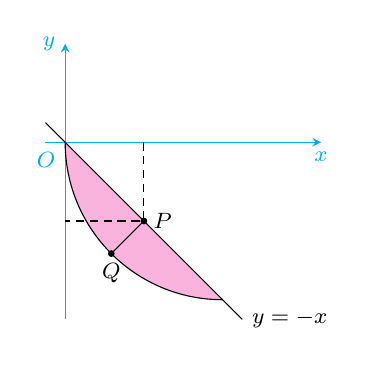
\begin{tikzpicture}[->,samples=100,>=stealth,domain=-0.25:2.25,font=\footnotesize]
                \coordinate (xMin) at (-0.25,0);
                \coordinate (xMax) at (3.25,0);
                \coordinate (yMin) at (0,-2.25);
                \coordinate (yMax) at (0,1.25);
                \draw[->, cyan] (xMin)--(0,0) node [below left] {$O$}--(xMax) node[below] {$x$};
                \draw[->, cyan] (yMin)--(yMax) node [left] {$y$};
                %\draw[black] (2,0) circle (2);
                \draw[fill=magenta!30,-] (0,0) arc(180:270:2);
                \draw[-] plot(\x,-\x) node[right] {$y=-x$};
                \draw[densely dashed,-] (1,0) -- (1,-1) node [right] {$P$} -- (0,-1);
                \draw[fill=black] (1,-1) circle(1pt); \draw[fill=black] (0.586,-1.414) circle(1pt);
                \draw[-] (1,-1) -- (0.586,-1.414) node [below] {$Q$};
            \end{tikzpicture}
        \end{figure}
    \end{minipage}\hfill
    \begin{minipage}{0.68\linewidth}
        \begin{enumerate}[label=(\arabic{*})]
            \item $P$ 点的坐标为 $\qty(\dfrac{t}{\sqrt{2}},-\dfrac{t}{\sqrt{t}})$, 所以直线 $PQ$ 的方程为 $$y=x-\sqrt{2}~ (0\leqslant t\leqslant 2\sqrt{2})$$
                  由 $\begin{cases}
                          y=x-\sqrt{2}t \\x^2+y^2=4x
                      \end{cases}$ 解得点 $Q$ 的横坐标为 $$x_Q=1+\dfrac{t}{\sqrt{2}}-\dfrac{1}{2}\sqrt{4+4\sqrt{2}t-2t^2}$$
                  所以 $|PQ|=\sqrt{2}\qty(\dfrac{t}{\sqrt{2}}-x_Q)=\sqrt{2}\qty(\dfrac{1}{2}\sqrt{4+4\sqrt{2}t-2t^2}-1).$
            \item 所求旋转体体积为
                  \begin{flalign*}
                      V & =\pi\int_{0}^{2\sqrt{2}}|PQ|^2\dd t=2\pi\int_{0}^{2\sqrt{2}}\qty(\dfrac{1}{2}\sqrt{4+4\sqrt{2}t-2t^2}-1)^2\dd t \\
                        & =\dfrac{20}{3}\sqrt{2}\pi-2\sqrt{2}\pi^2.
                  \end{flalign*}
        \end{enumerate}
    \end{minipage}
\end{solution}

\begin{example}
    求曲线 $y=\e^{-x}\sqrt{\sin x}~~(x\geqslant 0)$ 与 $x$ 轴围成区域绕 $x$ 轴旋转一周所得旋转体体积.
\end{example}
\begin{solution}
    由曲线可知定义域 $x\in\qty[2n\pi,(2n+1)\pi]~~(n=0,1,2,\cdots)$, 那么体积为
    \begin{flalign*}
        V_n & =\sum_{n=0}^{\infty}\int_{2n\pi}^{(2n+1)\pi}\pi y^2\dd x=\sum_{n=0}^{\infty}\int_{2n\pi}^{(2n+1)\pi}\pi\e^{-2x}\sin x\dd x=-\dfrac{\pi}{5}\sum_{n=0}^{\infty}\e^{-2x}(2\sin x+\cos x)\biggl |_{2n\pi}^{(2n+1)\pi}          \\
            & =\dfrac{\pi}{5}\sum_{n=0}^{\infty}\qty(\e^{-(4n+2)\pi}+\e^{-4n\pi})=\dfrac{\pi}{5}\sum_{n=0}^{\infty}\e^{-2n\pi}=\dfrac{\pi}{5}\cdot\lim_{n\to\infty}\dfrac{1-\e^{-2n\pi}}{1-\e^{-2\pi}}=\dfrac{\pi}{5\qty(1-\e^{-2\pi})}.
    \end{flalign*}
\end{solution}

\subsubsection{平面曲线的弧长}

\begin{theorem}[平面曲线弧长公式]
    \index{平面曲线弧长公式}若平面曲线的方程为 $y=f(x)~ (a\leqslant x\leqslant b)$, 则 $x$ 介于 $a$ 与 $b$ 之间的曲线弧长为:
    $$s=\int_{a}^{b}\sqrt{1+\qty(y')^2}\dd x=\int_{a}^{b}\sqrt{1+\qty[f'(x)]^2 }\dd x.$$
    若方程由极坐标给出: $r=r(\theta)~ (\alpha\leqslant \theta\leqslant \beta)$, 则 $\theta$ 介于 $\alpha$ 与 $\beta$ 之间的曲线弧长为:
    $$s=\int_{\alpha}^{\beta}\sqrt{r^2(\theta)+\qty[r'(\theta)]^2}\dd \theta.$$
    若方程由参数方程给出: $x=\varphi(t),~y=\psi(t)~ (\alpha\leqslant t\leqslant \beta)$, 则 $t$ 介于 $\alpha$ 与 $\beta$ 之间的曲线弧长为:
    $$s=\int_{\alpha}^{\beta}\sqrt{\qty[\varphi'(t)]^2+\qty[\psi'(t)]^2}\dd t.$$
\end{theorem}

\begin{example}
    计算 $\displaystyle \int_{L}|y|\dd s$, 其中 $L$ 为双纽线 $\qty(x^2+y^2)^2=a^2\qty(x^2-y^2)~~(a>0).$
\end{example}
\begin{solution}
    令 $\begin{cases}
            x=r\cos\theta \\
            y=r\sin\theta
        \end{cases}$ 代入直角坐标系方程, 得 $r^2=a^2\qty(\cos^2\theta-\sin^2\theta)=a^2\cos 2\theta$, 由 $r=0$ 得 $\theta=\dfrac{\pi}{4}$, 从而双纽线在第一象限部分的方程为 $r^2=a^2\cos2\theta,~0\leqslant\theta\leqslant \dfrac{\pi}{4}$,
    并且 $$\dd s=\sqrt{r^2+\qty(r')^2}\dd \theta=\sqrt{a^2\cos2\theta+\dfrac{a^4\sin ^22\theta}{r^2}}\dd \theta=\dfrac{a}{\sqrt{\cos 2\theta}}\dd \theta$$
    由对称性 $\displaystyle \int_{L}|y|\dd s=4\int_{0}^{\frac{\pi}{4}}r\sin\theta\cdot\dfrac{a}{\sqrt{\cos 2\theta}}\dd \theta=4a^2\int_{0}^{\frac{\pi}{4}}\sin\theta\dd \theta=4a^2\qty(1-\dfrac{\sqrt{2}}{2})$.
\end{solution}

\begin{example}[2010 数二]
    当 $0\leqslant\theta\leqslant \pi$ 时, 求对数螺线 $r=\e^{\theta}$ 的弧长.
\end{example}
\begin{solution}
    $\displaystyle s=\int_{0}^{\pi}\sqrt{r^2+\qty(r')^2}\dd \theta=\sqrt{2}\int_{0}^{\pi}\e^\theta\dd \theta=\sqrt{2}\qty(\e^{\pi}-1).$
\end{solution}

\begin{example}[2011 数一]
    求曲面\label{tantdt} $\displaystyle y=\int_{0}^{x}\tan t\dd t~ \qty(0\leqslant x\leqslant \dfrac{\pi}{4})$ 的弧长 $s$.
\end{example}
\begin{solution}
    因为 $y'=\tan x$, 所以
    $$s=\int_{0}^{\frac{\pi}{4}}\sqrt{1+\tan^2x}\dd x=\int_{0}^{\frac{\pi}{4}}\sec x\dd x=\eval{\ln|\sec x+\tan x|}_{0}^{\frac{\pi}{4}}=\ln\qty(1+\sqrt{2}).$$
\end{solution}

\begin{example}[2019 数二]
    求曲线 $y=\ln\cos x\qty(0\leqslant x\leqslant \dfrac{\pi}{6})$ 的弧长.
\end{example}
\begin{solution}
    与例题 \ref{tantdt} 同样地, $\displaystyle s=\int_{0}^{\frac{\pi}{6}}\sqrt{1+\tan^2x}\dd x=\dfrac{1}{2}\ln 3.$
\end{solution}

\begin{example}
    点 $P$ 在曲线 $\begin{cases}
            x=a\cos ^3t \\
            y=a\sin ^3t
        \end{cases}t\in\qty[0,\dfrac{\pi}{2}],a>0$ 上两点 $A(a,0)$ 与 $B(0,a)$ 之间, 并且曲线 $BP$ 的长度是曲线 $AP$ 长度的 3 倍, 求 $P$ 点坐标.
\end{example}
\begin{solution}
    设 $P$ 点坐标为 $(a\cos^3t_0,a\sin^3t_0)$, 并且弧微分
    \begin{flalign*}
        \dd s=\sqrt{\qty[x'(t)]^2+\qty[y'(t)]^2}\dd t=\sqrt{\qty(-3a\cos^2t\cdot\sin t)^2+\qty(3a\sin^2t\cdot\cos t)^2}\dd t=\sqrt{9a^2\sin^2t\cos^2t}\dd t=\dfrac{3a}{2}|\sin 2t|\dd t
    \end{flalign*}
    则曲线 $AP$ 的长度是曲线 $AB$ 长度的 $\dfrac{1}{4}$, 因此有
    $$\int_{0}^{t_0}\dd s=\dfrac{1}{4}\int_{0}^{\frac{\pi}{2}}\dd s\Rightarrow \int_{0}^{t_0}\sin2t\dd t=\dfrac{1}{4}\int_{0}^{\frac{\pi}{2}}\sin 2t\dd t\Rightarrow \cos 2t_0=\dfrac{1}{2}\Rightarrow t_0=\dfrac{\pi}{6}$$
    于是 $P$ 点坐标为 $\qty(\dfrac{3\sqrt{3}a}{8},\dfrac{a}{8}).$
\end{solution}

\begin{example}
    求曲线弧 $r=a\sin^3\dfrac{\theta}{3}~~(a>0)$ 的全长.
\end{example}
\begin{errorSolution}
    弧微分 $\dd s=\sqrt{r^2(\theta)+\qty[r'(\theta)^2]}\dd \theta=\sqrt{a^2\sin^6\dfrac{\theta}{3}+a^2\sin^4\dfrac{\theta}{3}\cos^2\dfrac{\theta}{3}}\dd \theta=a\sin^2\dfrac{\theta}{3}\dd \theta$, 那么弧长为\\
    \begin{minipage}{0.24\linewidth}
        \begin{figure}[H]
            \centering
            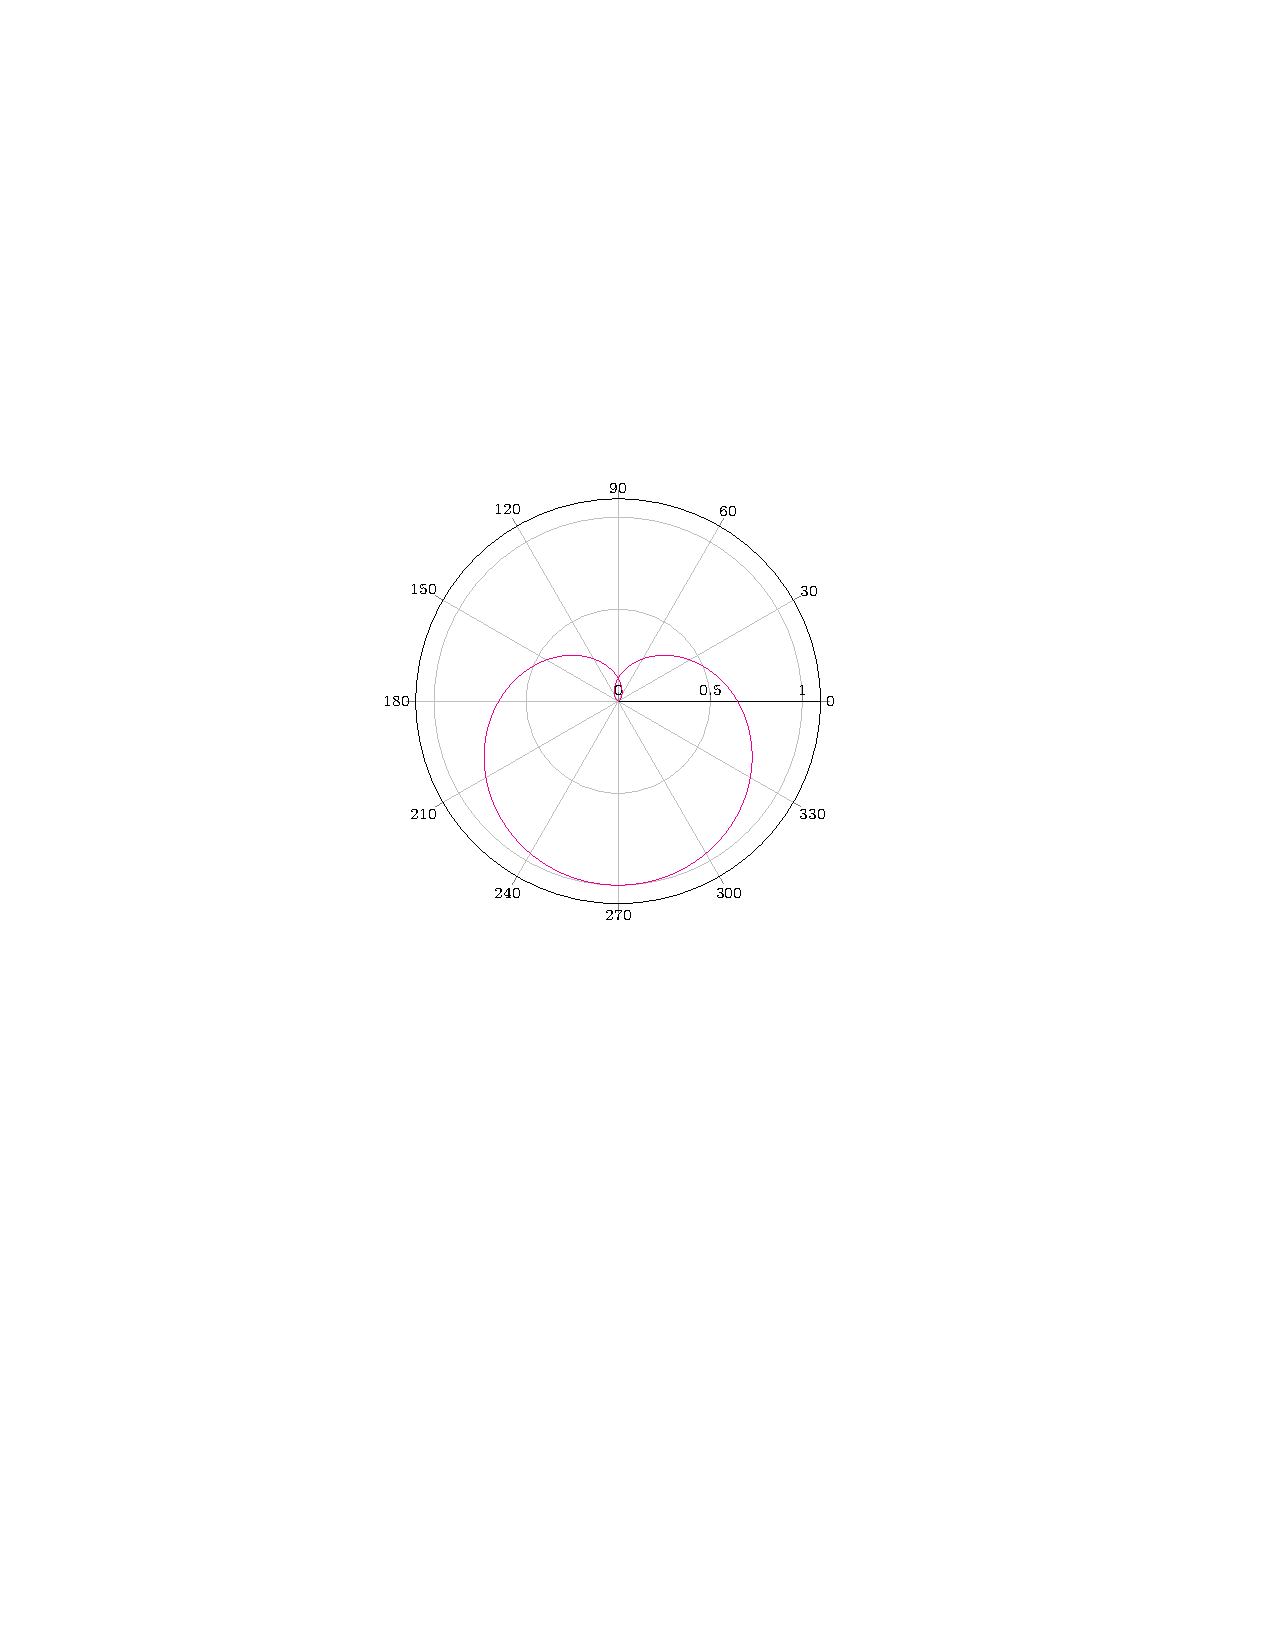
\includegraphics[scale=0.4]{figures/sin3 3pi.pdf}
            \caption{}
        \end{figure}
    \end{minipage}\hfill
    \begin{minipage}{0.75\linewidth}
        $$l=\int_{0}^{2\pi}a\sin^2\dfrac{\theta}{3}\dd \theta=a\int_{0}^{2\pi}\dfrac{1}{2}\qty(1-\cos\dfrac{2\theta}{3})\dd \theta=\eval{\dfrac{a}{2}\qty(\theta-\dfrac{3}{2}\sin\dfrac{2\theta}{3})}_{0}^{2\pi}=\pi a+\dfrac{3\sqrt{3}a}{8}.$$
        \textbf{错因: }$\theta$ 的变化范围并不是 $[0,2\pi]$, 事实上, 当 $\theta=0$ 时 $r=0$, 当 $\theta$ 从 0 开始增大时, $r$ 也从 $0$ 开始增大, 当 $\theta=\dfrac{3\pi}{2}$ 时, $r=a$ 达到最大; 根据对称性, 当 $\theta$ 继续增大时,  $\theta$ 减少, 当 $\theta$ 增大到 $3\pi$ 时, $r$ 减少到 0, 此时, 点 $(r,\theta)$ 的轨迹已经形成一条封闭曲线, 可见, $\theta$ 的变化范围是 $[0,3\pi]$.
    \end{minipage}
\end{errorSolution}
\begin{solution}
    $l=\displaystyle\int_{0}^{3\pi}a\sin^2\dfrac{\theta}{3}\dd \theta=\eval{\dfrac{a}{2}\qty(\theta-\dfrac{3}{2}\sin\dfrac{2\theta}{3})}_{0}^{3\pi}=\dfrac{3a\pi}{2}.$
\end{solution}

\begin{example}
    已知星形线 $\begin{cases}
            x=a\cos^3t \\ y=a\sin^3t
        \end{cases}(a>0)$ 求:
    \begin{enumerate}[label=(\arabic{*})]
        \item 它所围的面积;
        \item 它的弧长;
        \item 它绕 $x$ 轴旋转而成的旋转体的表面积.
    \end{enumerate}
\end{example}
\begin{solution}
    \begin{enumerate}[label=(\arabic{*})]
        \item $\displaystyle S=4\int_{0}^{a} y \dd x=4\int_{\frac{\pi}{2}}^{0} a\sin^3t\qty(-3a\cos^2t\sin t) \dd t=12a^2\int_{0}^{\frac{\pi}{2}} \sin^4t\cos^2t \dd t=\dfrac{3}{8}\pi a^2.$
        \item $\displaystyle L=4\int_{0}^{\frac{\pi}{2}} \sqrt{x'^2+y'^2} \dd t=4\int_{0}^{\frac{\pi}{2}} \sqrt{9a^2\cos^4t\sin^2t+9a^2\sin^4t\cos^2t} \dd t=12a\int_{0}^{\frac{\pi}{2}} \sin t \dd \sin t=6a.$
        \item $\displaystyle S=2\int_{0}^{a} 2\pi y\sqrt{1+\qty(y'_x)^2} \dd x=4\pi a\int_{0}^{\frac{\pi}{2}} \sin^3t\cdot 3a \cos t\sin t \dd t=\dfrac{12}{5}\pi a^2.$
    \end{enumerate}
\end{solution}

\begin{example}
    设心形线为 $r=a(1+\cos\theta)~ (a>0)$, 试用定积分计算:
    \begin{enumerate}[label=(\arabic{*})]
        \item 它所围成的图形的面积 $A$;
        \item 它的长度 $L$;
        \item 它所围成的图形 $D$ 的重心 ($D$ 的密度为 1);
        \item 它自身的重心 $C$;
        \item 它绕极轴旋转所得闭曲面所围立体的体积 $V$;
        \item 它绕极轴旋转所得闭曲面的面积 $S$;
        \item 它对极轴的转动惯量 $I$ (线密度为 1).
    \end{enumerate}
\end{example}
\begin{solution}
    \begin{minipage}{0.81\linewidth}
        \begin{enumerate}[label=(\arabic{*})]
            \item $\displaystyle A=2\cdot\dfrac{1}{2}\int_{0}^{\pi}a^2(1+\cos\theta)^2\dd \theta=a^2\int_{0}^{\pi}\qty(1+2\cos\theta+\cos^2\theta)\dd \theta=\dfrac{3\pi}{2}a^2$.
            \item $\displaystyle L=2\int_{0}^{\pi}\sqrt{r^2(\theta)+\qty[r'(\theta)]^2}\dd \theta=2\sqrt{2}a\int_{0}^{\pi}\sqrt{1+\cos\theta}\dd \theta=4a\int_{0}^{\pi}\cos\dfrac{\theta}{2}\dd \theta   =8a$.
            \item 设重心坐标 $C$ 为 $(\xi,\eta)$, $D$ 在极轴上方的一半区域为 $D_1$, 由对称性知 $\eta=0$, 下求 $\xi$, \newline
                  \textbf{法一: }用静力矩微元法, 这里从略.\newline
                  \textbf{法二: }利用二重积分求 $\xi$,
                  \begin{flalign*}
                      \xi & =\dfrac{1}{M}\iint\limits_{D_1}\rho x\dd \sigma=\dfrac{1}{M}\int_{0}^{\pi}\dd \theta\int_{0}^{a(1+\cos\theta)}r^2\cos\theta\dd r=\dfrac{a^3}{3M}\int_{0}^{\pi}(1+\cos\theta)^3\cos\theta\dd \theta \\
                          & =\dfrac{a^3}{3M}\int_{0}^{\pi}\qty(\cos\theta+3\cos^2\theta++3\cos^3\theta+\cos^4\theta)\dd \theta=\dfrac{5a}{6}
                  \end{flalign*}
                  其中 $M=\dfrac{1}{2}A\cdot\rho=\dfrac{1}{2}A=\dfrac{3\pi}{4}a^2.$
        \end{enumerate}
    \end{minipage}\hfill
    \begin{minipage}{0.18\linewidth}
        \begin{figure}[H]
            \centering
            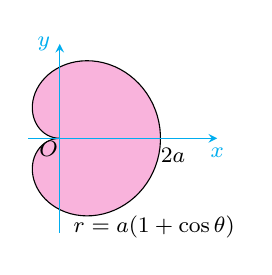
\begin{tikzpicture}[->,samples=100,>=stealth,scale=0.8,font=\footnotesize]
                \draw[-,domain=-pi:pi,fill=magenta!30]plot({1.6*cos(\x/2 r)*cos(\x r)},{1.6*cos(\x/2 r)*sin(\x r)});
                \draw[->,cyan](-0.5,0)--(2.5,0)node[below]{$x$};
                \draw[->,cyan](0,-1.5)--(0,1.5)node[left]{$y$};
                \node at(-5pt,-5pt){$O$};\node[below]at(1.8,0){$2a$};
                \node at(1.5,-1.4){$r=a(1+\cos\theta)$};
            \end{tikzpicture}
            \caption{}
        \end{figure}
    \end{minipage}
    \begin{enumerate}[label=(\arabic{*})]
        \setcounter{enumi}{3}
        \item 设心形线 $\Gamma$ 的上半条为 $\Gamma_1$, 设 $\Gamma,\Gamma_1$ 的重心分别为 $(\xi,\eta)$ 和 $(\xi_1,\eta_1)$, 由对称性知 $\xi=\xi_1,\eta=\eta_1=0$, 因为 $\Gamma_1$ 对 $y$ 轴的
              静力矩微元为 $$\dd M_y=r(\theta)\cos\theta\cdot\rho\dd s=r(\theta)\cos\theta\sqrt{r^2(\theta)+\qty[r'(\theta)]^2}\dd \theta$$
              从而, 有
              \begin{flalign*}
                  M_y & =\int_{0}^{\pi}\dd M_y=\int_{0}^{\pi}r(\theta)\cos\theta\sqrt{r^2(\theta)+\qty[r'(\theta)]^2}\dd \theta=\sqrt{2}a^2\int_{0}^{\pi}(1+\cos\theta)^{\frac{3}{2}}\cos\theta\dd \theta           \\
                      & =4a^2\int_{0}^{\pi}\qty(2\cos^5\dfrac{\theta}{2}-\cos^3\dfrac{\theta}{2})\dd \theta \xlongequal{\frac{\theta}{2}=t}8a^2\int_{0}^{\frac{\pi}{2}}\qty(2\cos^5t-\cos^3t)\dd t=\dfrac{16a^2}{5}
              \end{flalign*}
              由有 (2) 知, $\Gamma$ 的长度为 $8a$, 于是 $\Gamma$ 的质量为 $M=\dfrac{L}{2}\cdot\rho=4a$
              所以 $\xi=\dfrac{M_y}{M_1}=\dfrac{4a}{5}$, 从而知 $C\qty(\dfrac{4a}{5},0)$.
    \end{enumerate}
    \begin{minipage}{0.81\linewidth}
        \begin{enumerate}[label=(\arabic{*})]
            \setcounter{enumi}{4}
            \item 由 $r=a(1+\cos \theta)$ 可得 $$x=a(1+\cos \theta)\cos\theta=a\qty[\qty(\cos\theta+\dfrac{1}{2})^2-\dfrac{1}{4}]\geqslant-\dfrac{a}{4},~y=a(1+\cos\theta)\sin\theta$$
                  体积元 $\dd V=\pi y^2(\theta)\dd x(\theta)$, 于是
                  \begin{flalign*}
                      V & =\int_{\frac{2\pi}{3}}^{0}\pi y^2(\theta)\dd x(\theta)-\int_{\frac{2\pi}{3}}^{\pi}\pi y^2(\theta)\dd x(\theta)=\int_{\pi}^{0}y^2(\theta)\dd x(\theta)          \\
                        & =\int_{\pi}^{0}\pi\qty[a(1+\cos\theta)]^2\qty[a(1+\cos\theta)\cos\theta]'\dd \theta=\pi a^3\int_{0}^{\pi}\sin^3\theta(1+\cos\theta)^2(1+2\cos\theta)\dd \theta \\
                        & \xlongequal{\cos\theta=t}\pi a^3\int_{1}^{-1}\qty(t^2-1)(1+t)^2(1+2t)\dd t=\pi a^3\int_{-1}^{1}\qty(1+4t^2-5t^4)\dd t=\dfrac{8\pi}{3}a^3.
                  \end{flalign*}
            \item 因为 $\dd S=2\pi y(\theta)\dd s(\theta)=2\pi r(\theta)\sin \theta\sqrt{r^2(\theta)+\qty[r'(\theta)]^2}\dd \theta$, 所以, 有
                  \begin{flalign*}
                      S & =\int_{0}^{\pi}2\pi r(\theta)\sin \theta\sqrt{r^2(\theta)+\qty[r'(\theta)]^2}\dd \theta=2\sqrt{2}\pi a^2\int_{0}^{\pi}\sin\theta(1+\cos\theta)^{\frac{3}{2}}\dd \theta \\
                        & =-2\sqrt{2}\pi a^3\int_{0}^{\pi}(1+\cos\theta)^{\frac{3}{2}}\dd (1+\cos\theta)=\dfrac{32\pi}{5}a^2.
                  \end{flalign*}
            \item 因为 $\dd I=y^2(\theta)\rho \dd s(\theta)=r^2(\theta)\sin^2\theta\sqrt{r^2(\theta)+\qty[r'(\theta)]^2}\dd \theta$, 所以, 有
                  \begin{flalign*}
                      I & =2\int_{0}^{\pi}r^2(\theta)\sin^2\theta\sqrt{r^2(\theta)+\qty[r'(\theta)]^2}\dd \theta=2\sqrt{2}a^3\int_{0}^{\pi}\sin^2\theta(1+\cos\theta)^{\frac{5}{2}}\dd \theta                        \\
                        & =64a^3\int_{0}^{\pi}\sin^2\dfrac{\theta}{2}\cos^7\dfrac{\theta}{2}\dd \theta \xlongequal{\frac{\theta}{2}=t}128a^3\int_{0}^{\frac{\pi}{2}}\qty(\cos^7t-\cos^9t)\dd t=\dfrac{2048}{315}a^3.
                  \end{flalign*}
        \end{enumerate}
    \end{minipage}\hfill
    \begin{minipage}{0.18\linewidth}
        \begin{figure}[H]
            \centering
            \tdplotsetmaincoords{70}{135}
            \begin{tikzpicture}[line join=bevel,tdplot_main_coords,->,samples=100,>=stealth,fill opacity=.5,scale=0.8,font=\footnotesize]
                \coordinate (xMin) at ( -1.75,   0,  0);
                \coordinate (xMax) at ( 1.5,    0,  0);
                \coordinate (yMin) at ( 0,  -1.75,   0);
                \coordinate (yMax) at ( 0,  1.5,    0);
                \coordinate (zMin) at ( 0,  0,  -1);
                \coordinate (zMax) at ( 0,  0,  2.3);
                \pgfsetlinewidth{.1pt}
                \tdplotsphericalsurfaceplot[parametricfill]{72}{36}{1+1*cos(\tdplottheta)}{black}{\tdplotphi}%
                {\draw[->, cyan] (xMin) -- (0,0,0) node [below right] {$O$} -- (xMax) node[anchor=north east]{$y$};}
                {\draw[->, cyan] (yMin) -- (0,0,0) -- (yMax) node[anchor=north west]{$z$};}
                {\draw[->, cyan] (zMin) -- (0,0,0) -- (zMax) node[anchor=south]{$x$};}
            \end{tikzpicture}
            \caption{}
        \end{figure}
    \end{minipage}
\end{solution}

\subsection{定积分的物理应用}

\subsubsection{变力所做的功}

\begin{theorem}[变力的功]
    若质点沿变力 $F(x)$ 方向从 $x=a$ 到 $x=b$ 做直线运动, 则变力所做的功为:
    $$W=\int_{a}^{b}F(x)\dd x.$$
\end{theorem}

\subsubsection{物体的质量与重心}

\begin{theorem}[质量与重心坐标公式]
    若 $f(x)$ 代表细棒的质量密度, 细棒所占区间为 $[a,b]$, 则细棒的质量为:
    $$M=\int_{a}^{b}f(x)\dd x.$$
    重心坐标为:
    $$\overline{x}=\dfrac{1}{M}\int_{a}^{b}xf(x)\dd x.$$
\end{theorem}

\subsection{定积分综合性问题}

\subsubsection{积分等式命题的证明}

\begin{example}
    设 $ f(x) $ 在 $ [a, b] $ 上有二阶导数, 且 $ f^{\prime \prime}(x) $ 在 $ [a, b] $ 上黎曼可积, 证明:
    $$f(x)=f(a)+f^{\prime}(a)(x-a)+\int_{a}^{x}(x-t) f^{\prime \prime}(t) \dd  t, \forall x \in[a, b] .$$
\end{example}
\begin{proof}[{\songti \textbf{证法一}}]
    由 N-L 公式,
    \begin{flalign*}
        f(x) & =f(a)+\int_{a}^{x}f'(t)\dd t=f(a)+\int_{a}^{x}f'(a)\dd t+\int_{a}^{x}\dd t\int_{a}^{t}f''(u)\dd u \\
             & =f(a)+f'(a)(x-a)+\int_{a}^{x}\dd t\int_{t}^{x}f''(u)\dd u=f(a)+f'(a)(x-a)+\int_{a}^{x}(x-t).
    \end{flalign*}
\end{proof}
\begin{proof}[{\songti \textbf{证法二}}]
    即证 $\displaystyle \int_{a}^{x}(x-t)f''(t)\dd t=f(x)-f(a)-f'(a)(x-a)$, 由表格积分法:
    \begin{table}[H]
        \centering
        \begin{tabular}{l| c c c}
            $f'$   & $(x-t)$     & $1$         & $0$    \\
            \midrule
                   & $+\searrow$ & $-\searrow$          \\
            \midrule
            $\int$ & $f''(t)$    & $f'(t)$     & $f(t)$
        \end{tabular}
    \end{table}
    于是 $\displaystyle \int_{a}^{x}(x-t)f''(t)\dd t=[(x-t)f'(t)-f(t)]_a^x=-f(x)-(x-a)f'(a)+f(a)$, 整理得证.
\end{proof}

\begin{example}
    设 $f(x)\in D(0,1),~f(0)=f(1)=-2,~\displaystyle\int_{0}^{1}f(x)\dd x=0$, 证明: $\exists\xi\in(0,1)$, 使得 $$f'(\xi)-f(\xi)=\xi.$$
\end{example}
\begin{proof}[{\songti \textbf{证}}]
    令 $F(x)=\e^{-x}(f(x)+x+1)$, 有 $F(0)=-1,~F(1)=0$, 因为 $\displaystyle\int_{0}^{1}f(x)\dd x=0$, 由积分中值定理知, $\exists\eta\in(0,1)$, 使得
    $$\displaystyle\int_{0}^{1}f(x)\dd x=f(\eta)\int_{0}^{1}\dd x=f(\eta)=0$$
    而 $F(\eta)=\e^{-\eta}(f(\eta)+\eta+1)>0$, 因此 $\exists\xi\in(0,1)$, 使得 $F(x)\leqslant F(\xi)$, 即 $F(x)$ 的最大值一定在区间 $(0,1)$ 内取到,
    由 Fermat 引理知, $F'(\xi)=0$, 即 $$\eval{-\e^{-x}(f(x)+x+1)+\e^{-x}(f'(x)+1)}_{x=\xi}=f'(\xi)-f(\xi)=\xi.$$
\end{proof}

\begin{example}
    设 $f(x)$ 在 $[2,4]$ 上二阶连续可导, $f(3)=0$, 证明: $\exists\xi\in(2,4)$, 使得 $\displaystyle f''(\xi)=3\int_{2}^{4}f(x)\dd x.$
\end{example}
\begin{proof}[{\songti \textbf{证}}]
    构造 $\displaystyle F(x)=\int_{2}^{x}f(t)\dd t$, 那么将  $F(2),F(4)$ 分别在 $x=3$ 处 Taylor 展开, 有
    \begin{flalign*}
        F(2)=F(3)+F'(3)(2-3)+\dfrac{1}{2!}F''(3)(2-3)^2+\dfrac{1}{3!}F'''(\xi_1)(2-3)^3 \\
        F(4)=F(3)+F'(3)(4-3)+\dfrac{1}{2!}F''(3)(4-3)^2+\dfrac{1}{3!}F'''(\xi_2)(4-3)^3
    \end{flalign*}
    注意到 $F(2)=F'(3)=0$, 那么上式化为 $\begin{cases}
            0=F(3)+\dfrac{1}{2}F''(3)-\dfrac{1}{6}F'''(\xi_1) \\[6pt]
            F(4)=F(3)+\dfrac{1}{2}F''(3)+\dfrac{1}{6}F'''(\xi_2)
        \end{cases}$
    即 $$F(4)=\dfrac{1}{6}\qty(F'''(\xi_1)+F'''(\xi_2))$$
    因为 $F'''(x)=f''(x)$ 在 $[2,4]$ 上连续, 故 $F'''(x)$ 在 $[2,4]$ 上有最大值 $M$ 和最小值 $m$, 使得
    $$m\leqslant \dfrac{1}{2}\qty(F'''(\xi_1)+F'''(\xi_2))\leqslant M$$
    又由连续函数的介值定理知 $\exists\xi\in(\xi_1,\xi_2)\subset(2,4)$, 使得 $$F'''(\xi)=\dfrac{1}{2}\qty(F'''(\xi_1)+F'''(\xi_2))$$
    故 $F(4)=\dfrac{1}{3}\cdot\dfrac{1}{2}\qty(F'''(\xi_1)+F'''(\xi_2))=\dfrac{1}{3}F'''(\xi)$, 则
    $$F'''(\xi)=3F(4)\Rightarrow f''(\xi)=3\int_{2}^{4}f(x)\dd x.$$
\end{proof}

\begin{example}
    设 $f(x)$ 在 $[-1,1]$ 二阶导函数连续, 证明: $\exists\xi\in[-1,1]$, 使得 $$\displaystyle\int_{-1}^{1}xf(x)\dd x=\dfrac{1}{3}[2f'(\xi)+\xi f''(\xi)].$$
\end{example}
\begin{proof}[{\songti \textbf{证}}]
    构造 $F(x)=xf(x)$, 那么 $F(x)$ 在 $[-1,1]$ 二阶导函数连续, 并且 $$F'(x)=f(x)+xf'(x),~F''(x)=2f'(x)+xf''(x)$$
    又由 Taylor 展开得,
    $$F(x)=F(0)+F'(0)x+\dfrac{1}{2!}F''(\theta x)x^2~ \theta\in(0,1)$$
    且 $F(0)=0,F'(0)=f(0)x$, 于是 $F(x)=f(0)x+\dfrac{1}{2}F''(\theta x)x^2$, 两边对 $x$ 积分, 则有,
    $$\int_{-1}^{1}F(x)\dd x=\int_{-1}^{1}f(0)x\dd x+\dfrac{F''(\theta x)}{2}\int_{-1}^{1}x^2\dd x=\dfrac{F''(\theta x)}{2}\int_{-1}^{1}x^2\dd x$$
    记 $m=\min\limits_{0\leqslant x\leqslant 1}F''(x),~M=\max\limits_{0\leqslant x\leqslant 1}F''(x)$, 于是
    $$m\int_{-1}^{1}x^2\dd x\leqslant \int_{-1}^{1}F''(\theta x)x^2\dd x\leqslant M\int_{-1}^{1}x^2\dd x$$
    即 $\dfrac{2}{3}m\leqslant\displaystyle\int_{-1}^{1}F''(\theta x)x^2\dd x\leqslant \dfrac{2}{3}M$,
    因此有 $\displaystyle m\leqslant \int_{-1}^{1}F(x)\dd x\leqslant M$, 对 $F''(x)$ 利用连续函数的介值定理, 即 $\exists\xi\in[-1,1]$, 使得 $3\displaystyle\int_{-1}^{1}F(x)\dd x=F''(\xi)$, 即得证.
\end{proof}

\begin{example}
    已知 $f(x)$ 在 $[a,b]$ 上二阶可导, $f(a)=f(b)=0$, 试证: $\exists \xi\in(a,b)$, 使得 $$\int_{a}^{b}f(x)\dd x=\frac{1}{12}f''(\xi)(a-b)^3.$$
\end{example}
\begin{proof}[{\songti \textbf{证}}]
    令 $\displaystyle F(x)=\int_{a}^{x}f(t)\dd t-\frac{1}{2}(x-a)f(x)$, $\displaystyle G(x)=-\frac{1}{12}(x-a)^3$,
    在 $[a,b]$ 上连续两次应用 Cauchy 中值定理,
    \begin{flalign*}
        \dfrac{\displaystyle\int_{a}^{b}f(x)\dd x-0}{-\dfrac{1}{12}(b-a)^3-0} & =\dfrac{F(b)-F(a)}{G(b)-G(a)}\xlongequal[a\leqslant \xi_1\leqslant b]{\text{Cauchy 中值定理}}\dfrac{F"(\xi_1)}{G'(\xi_1)}                                                                                                    \\
                                                                              & =\dfrac{\dfrac{1}{2}f(\xi_1)-\dfrac{1}{2}(\xi_1-a)f'(\xi)-0}{-\dfrac{1}{4}(\xi_1-a)^2-0}\xlongequal[a\leqslant\xi\leqslant\xi_1]{\text{Cauchy 中值定理}}\dfrac{-\dfrac{1}{2}f''(\xi)(\xi-a)}{-\dfrac{1}{2}(\xi-a)}=f''(\xi).
    \end{flalign*}
    此式同乘 $\displaystyle-\frac{1}{12}(b-a)^3=\frac{1}{12}(b-a)^3$, 即得所求.
\end{proof}

\begin{example}
    设函数 $f(x)$ 在 $[a,b]$ 上二阶可导, 证明至少存在一点 $\xi\in(a,b)$, 使得
    $$\int_{a}^{b}f(x)\dd x=f(b)(b-a)-f'(b)\dfrac{(b-a)^2}{2}+\dfrac{1}{6}(b-a)^3f''(\xi).$$
\end{example}
\begin{proof}[{\songti \textbf{证}}]
    令 $k$ 为使 $\displaystyle \int_{a}^{b}f(x)\dd x=f(b)(b-a)-f'(b)\dfrac{(b-a)^2}{2}+\dfrac{1}{6}(b-a)^3k$ 成立的实常数, 构造辅助函数
    $$F(x)=\int_{a}^{x}f(t)\dd t-f(x)(x-a)+f'(x)\dfrac{(x-a)^2}{2}-\dfrac{1}{6}(x-a)^3k$$
    则 $F(a)=F(b)=0$, 故由 Rolle 定理知 $\exists\xi\in(a,b)$, 使 $F'(\xi)=0$, 即
    $$F'(\xi)=f''(\xi)\dfrac{(\xi-a)^2}{2}-\dfrac{1}{2}(\xi-a)^2k=0$$
    得证 $k=f''(\eta)$, 故得证.
\end{proof}

\begin{example}
    设函数 $f(x)$ 在 $[a,b]$ 上具有二阶连续的导数, 证明存在 $\xi\in(a,b)$, 使得
    $$\int_{a}^{b}f(x)\dd x=(b-a)f\qty(\dfrac{a+b}{2})+\dfrac{1}{24}(b-a)^3f''(\xi).$$
\end{example}
\begin{proof}[{\songti \textbf{证法一}}]
    将 $f(x)$ 在 $\dfrac{a+b}{2}$ 处进行 Taylor 展开, 有
    $$f(x)=f\qty(\dfrac{a+b}{2})+f'\qty(\dfrac{a+b}{2})\qty(x-\dfrac{a+b}{2})+\dfrac{f''(\xi_1)}{2!}\qty(x-\dfrac{a+b}{2})$$
    因为 $f''(x)$ 在 $[a,b]$ 上连续, 所以存在最小值 $m$ 和最大值 $M$, 使 $\forall x\in[a,b]$, $m\leqslant f''(x) \leqslant M$, 于是
    $$m\int_{a}^{b}\qty(x-\dfrac{a+b}{2})^2\dd x\leqslant \int_{a}^{b}f''(\xi_1)\qty(x-\dfrac{a+b}{2})^2\dd x\leqslant M\int_{a}^{b}\qty(x-\dfrac{a+b}{2})^2\dd x$$
    从而 $\displaystyle m\leqslant \dfrac{\displaystyle \int_{a}^{b}f''(\xi_1)\qty(x-\dfrac{a+b}{2})^2\dd x}{\displaystyle \int_{a}^{b}\qty(x-\dfrac{a+b}{2})^2\dd x}\leqslant M$, 故由介值定理知, 存在 $\xi\in(a,b)$, 使得
    $$f''(\xi)=\dfrac{\displaystyle\int_{a}^{b}f''(\xi_1)\qty(x-\dfrac{a+b}{2})^2\dd x}{\displaystyle \int_{a}^{b}\qty(x-\dfrac{a+b}{2})^2\dd x}$$
    即得证 $\displaystyle\int_{a}^{b}f(x)\dd x=(b-a)f\qty(\dfrac{a+b}{2})+\dfrac{1}{24}(b-a)^3f''(\xi).$
\end{proof}
\begin{proof}[{\songti \textbf{证法二}}]
    令 $\displaystyle F(x)=\int_{a}^{x}f(t)\dd t$, 将 $F(x)$ 在 $x_0=\dfrac{a+b}{2}$ 处 Taylor 展开得
    $$F(x)  =F\left( x_{0}\right) +F'\left( x_{0}\right) \left( x-x_{0}\right) +\dfrac{F''(x)  }{2!}\left( x-x_{0}\right) ^{2}+\dfrac{F'''\left( \xi \right) }{3!}\left( x-x_{0}\right) ^{3}$$
    其中 $\xi$ 介于 $x_0$ 与 $x$ 之间, 将 $x=a$ 和 $x=b$ 代入上式, 并相减得
    $$F\left( b\right) -F\left( a\right) =\left( b-a\right) f\left( \dfrac{a+b}{2}\right) +\dfrac{1}{24}\left( b-a\right) ^{3}\dfrac{f''\left( \xi _{1}\right) +f''\left( \xi _{2}\right) }{2}$$
    其中 $a <\xi _{2} <\dfrac{a+b}{2} <\xi _{1} <b$, 不妨设 $f''(\xi_1)\leqslant f''(\xi_2)$, 则 $f''(x_1)\leqslant \dfrac{f''(\xi_1)+f''(\xi_2)}{2}\leqslant f''(\xi_2)$, 由导函数 $f''(x)$ 的 Darboux 定理或 $f''(x)$ 的连续性及介值定理知,
    $\exists\xi\in(\xi_1,\xi_2)$ 或 $(\xi_2,\xi_1)\subset (a,b)$, 使 $f''(\xi)=\dfrac{f''(\xi_1)+f''(\xi_2)}{2}$, 故 $\displaystyle\int_{a}^{b}f(x)\dd x=(b-a)f\qty(\dfrac{a+b}{2})+\dfrac{1}{24}(b-a)^3f''(\xi).$
\end{proof}
\begin{proof}[{\songti \textbf{证法三}}]
    设 $ k $ 为使 $ \displaystyle \int_{a}^{b} f(x) \dd  x=(b-a) f\left(\frac{a+b}{2}\right)+\frac{1}{24}(b-a)^{3} k $ 成立的实数, 要证结论成立, 只需证 $k=f''(\xi)$, 为此构造辅助函数
    $$ \displaystyle F(x)=\int_{a}^{x} f(t) \dd  t-(x-a) f\left(\frac{a+x}{2}\right)-\frac{1}{24}(x-a)^{3} k $$
    则 $ F(a)=F(b)=0 $, 故由 Rolle 定理, $\exists \eta \in(a, b) $, 使 $ F^{\prime}(\eta)=0 $, 即
    $$f(\eta)-f\left(\frac{a+\eta}{2}\right)-\frac{\eta-a}{2} f^{\prime}\left(\frac{a+\eta}{2}\right)-\frac{k}{8}(\eta-a)^{2}=0 $$
    又将 $ f(\eta) $ 在 $ x=\dfrac{a+\eta}{2} $ 处进行 Taylor 展开, 有
    $$f(\eta)=f\left(\dfrac{a+\eta}{2}\right)+f^{\prime}\left(\frac{a+\eta}{2}\right) \frac{\eta-a}{2}+\frac{f^{\prime \prime}(\xi)}{2 !}\left(\frac{\eta-a}{2}\right)^{2}$$
    其中 $ \xi \in\left(\dfrac{a+\eta}{2}, \eta\right) \subset(a, b) $,
    比较上述两式, 得 $ k=f^{\prime \prime}(\xi) $ 故得证.
\end{proof}
\begin{proof}[{\songti \textbf{证法四}}]
    取 $\rho\equiv1$, 首先构造数值求积公式 $\displaystyle\int_{a}^{b}f(x)\dd x\approx A_0f\qty(\dfrac{a+b}{2})$, 使其具有尽可能高的代数精度,
    为此, 取 $f(x)=1$ 使求积公式精确成立, 则有 $$A_0=b-a$$
    把 $A_0$ 代入求积公式, 取 $f(x)=x$, 代入验算知求积公式精确成立; 再取 $f(x)=x^2$, 求积公式不精确成立,
    故求积公式 $\displaystyle\int_{a}^{b}f(x)\dd x\approx (b-a)f\qty(\dfrac{a+b}{2})$ 的代数精度为 $1$;
    其次, 构造一次插值多项式
    $$P_1\qty(\dfrac{a+b}{2})=f\qty(\dfrac{a+b}{2}),~P'_1\qty(\dfrac{a+b}{2})=f'\qty(\dfrac{a+b}{2})$$
    那么 $W_2(x)=\qty(x-\dfrac{a+b}{2})^2$ 且不恒为 $0$, 又
    $$K=\int_{a}^{b}W_2(x)\dd x=\dfrac{1}{12}(b-a)^3$$
    那么至少存在一点 $\xi\in(a,b)$, 使得 $$\int_{a}^{b}f(x)\dd x=(b-a)f\qty(\dfrac{a+b}{2})+\dfrac{f''(\xi)}{2!}\cdot\dfrac{1}{12}(b-a)^3$$
    即得待证等式.
\end{proof}

\begin{example}
    设函数 $f(x)$ 在 $[a,b]$ 上具有二阶连续的导数, 证明存在一点 $\xi\in(a,b)$, 使得
    $$\int_{a}^{b}f(x)\dd x=\dfrac{b-a}{2}(f(a)+f(b))-\dfrac{1}{12}f''(\xi)(b-a)^3.$$
\end{example}
\begin{proof}[{\songti \textbf{证法一}}]
    设 $k$ 为使 $\displaystyle \int_{a}^{b}f(x)\dd x=\dfrac{b-a}{2}(f(a)+f(b))-\dfrac{1}{12}k(b-a)^3$ 成立的实常数, 则证 $k=f''(\xi)$, 为此构造辅助函数
    $$F(x)=\int_{a}^{x}f(t)\dd t-\dfrac{x-a}{2}(f(a)+f(x))+\dfrac{1}{12}k(x-a)^3$$
    那么 $F(a)=F(b)=0$, 由 Rolle 定理知, $\exists\xi_1\in(a,b)$, 使得 $F'(\xi_1)=0$, 又
    $$F'(x)=f(x)-\dfrac{1}{2}(f(x)+f(a))-\dfrac{x-a}{2}f'(x)+\dfrac{1}{4}k(x-a)^2$$
    并且注意到 $F'(a)=F'(\xi_1)=0$, 再由 Rolle 定理知, $\exists\xi\in(a,\xi_1)\subset(a,b)$, 使得 $F''(\xi)=0$, 并且
    $$F''(\xi)=-\dfrac{\xi-a}{2}f''(\xi)+\dfrac{1}{2}k(\xi-a)=0$$
    即得证 $k=f''(\xi).$
\end{proof}
\begin{proof}[{\songti \textbf{证法二}}]
    取 $\rho(x)\equiv1$, 首先构造数值求积公式 $\displaystyle\int_{a}^{b}f(x)\dd x\approx A_0f(a)+A_1f(b)$, 使其具有尽可能高的代数精度, 为此,
    分别取 $f(x)=1,x$ 使求积公式精确成立, 则有 $$\left\{\begin{matrix}
            A_0  & + & A_1  & = & b-a                \\
            aA_0 & + & bA_1 & = & \dfrac{b^2-a^2}{2}
        \end{matrix}\right.\Rightarrow A_0=A_1=\dfrac{b-a}{2} $$
    把 $A_0,~A_1$ 代入求积公式, 取 $f(x)=x^2$, 代入验算知求积公式精确成立; 再取 $f(x)=x^3$, 求积公式不精确成立,
    故求积公式 $\displaystyle\int_{a}^{b}f(x)\dd x\approx\dfrac{b-a}{2}(f(a)+f(b))$ 的代数精度为 $2$;
    其次, 构造二次插值多项式 $P_1(x)$, 使满足 $$P_1(a)=f(a),~P'_1(b)=f'(b)$$
    那么 $W_2(x)=(x-a)(x-b)\geqslant 0$ 且不恒为 $0$, 又
    $$K=\int_{a}^{b}W_2(x)\dd x=-\dfrac{1}{6}(b-a)^3$$
    那么至少存在一点 $\xi\in(a,b)$, 使得
    $$\int_{a}^{b}f(x)\dd x=\dfrac{b-a}{2}(f(a)+f(b))-\dfrac{f''(\xi)}{2!}\cdot\dfrac{1}{6}(b-a)^3$$
    即得待证等式.
\end{proof}

\begin{example}
    设函数 $f(x)$ 在 $[a,b]$ 上有三阶连续的导数, 证明至少存在一点 $\eta\in(a,b)$, 使得
    $$\int_{a}^{b}f(x)\dd x=\dfrac{b-a}{4}\qty[f(a)+3f\qty(\dfrac{a+2b}{3})]+\dfrac{(b-a)^4}{216}f'''(\eta).$$
\end{example}
\begin{proof}[{\songti \textbf{证}}]
    令 $k$ 为使 $\displaystyle\int_{a}^{b}f(x)\dd x=\dfrac{b-a}{4}\qty[f(a)+3f\qty(\dfrac{a+2b}{3})]+\dfrac{(b-a)^4}{216}k$ 成立的实常数, 要证结论成立, 只需证 $k=f'''(\eta)$,
    为此, 将上式右端移到左端, 并将 $b$ 改写为 $x$, 构造辅助函数
    $$F(x)=\int_{a}^{x}f(t)\dd t-\dfrac{x-a}{4}\qty[f(a)+3f\qty(\dfrac{a+2x}{3})]-\dfrac{(x-a)^4}{216}k,~x\in[a,b]$$
    则 $F(a)=F(b)=0$, $F(x)$ 在 $[a,b]$ 上连续且可导, 由 Rolle 定理, $\exists\xi_1\in(a,b)$, 使得 $F'(\xi_1)=0$, 又
    $$F'(x)=f(x)-\dfrac{1}{4}\qty[f(a)+3f\qty(\dfrac{a+2x}{3})]-\dfrac{x-a}{2}f'\qty(\dfrac{a+2x}{3})-\dfrac{(x-a)^3}{54}k$$
    得 $F'(a)=F'(\xi_1)=0$, 故对 $F'(x)$ 在 $[a,\xi_1]$ 上用 Rolle 定理, 得 $\exists\xi_2\in(a,\xi_1)\subset(a,b)$, 使得 $F''(\xi_2)=0$, 即
    $$F''(\xi_2)=f'(\xi_2)-f'\qty(\dfrac{a+2\xi_2}{3})-\dfrac{\xi_2-a}{3}f''\qty(\dfrac{a+2\xi_2}{3})-\dfrac{(\xi_2-a)^2}{18}k=0$$
    再将 $f'(\xi_2)$ 在 $x=\dfrac{a+2\xi_2}{3}$ 处 Taylor 展开, 有
    $$f'(\xi_2)=f'\qty(\dfrac{a+2\xi_2}{3})+f''\qty(\dfrac{a+2\xi_2}{3})\qty(\xi_2-\dfrac{a+2\xi_2}{3})+\dfrac{1}{2!}f'''(\eta)\qty(\xi_2-\dfrac{a+2\xi_3}{3})^2$$
    其中 $\eta\in\qty(\dfrac{a+2\xi_2}{3})\subset(a,b)$, 比较上述两式, 即得 $k=f'''(\eta)$, 故得证.
\end{proof}

\begin{example}
    设函数 $f(x)$ 在 $[a,b]$ 上有三阶连续的导数, 证明至少存在一点 $\xi\in(a,b)$, 使得
    $$\int_{a}^{b}f(x)\dd x=\dfrac{b-a}{4}\qty[3f\qty(\dfrac{2a+b}{3})+f(b)]-\dfrac{(b-a)^4}{216}f'''(\xi).$$
\end{example}
\begin{proof}[{\songti \textbf{证}}]
    令 $k$ 为使 $\displaystyle \int_{a}^{b}f(x)\dd x=\dfrac{b-a}{4}\qty[3f\qty(\dfrac{2a+b}{3})+f(b)]-\dfrac{(b-a)^4}{216}k$ 成立的实常数, 要证结论成立, 只需证 $k=f'''(\eta)$,
    为此, 构造辅助函数 $$F(x)=\int_{x}^{b}f(t)\dd t-\dfrac{b-x}{4}\qty[3f\qty(\dfrac{2x+b}{3})+f(b)]+\dfrac{(b-x)^4}{216}k$$
    则 $F(a)=F(b)=0$, $F(x)$ 在 $[a,b]$ 上连续且可导, 由 Rolle 定理, $\exists\xi_1\in(a,b)$, 使得 $F'(\xi_1)=0$, 又
    $$F'(x)=-f(x)+\dfrac{1}{4}\qty[3f\qty(\dfrac{2x+b}{3})+f(b)]-\dfrac{b-x}{2}f'\qty(\dfrac{2x+b}{3})-\dfrac{(b-x)^3}{54}k$$
    得 $F'(\xi_1)=F'(b)=0$, 故对 $F'(x)$ 在 $[\xi_1,b]$ 上用 Rolle 定理, 得 $\exists\xi_2\in(\xi_1,b)\subset(a,b)$, 使得 $F''(\xi_2)=0$, 即
    $$F''(\xi_2)=-f'(\xi_2)+f'\qty(\dfrac{2\xi_2+b}{3})-\dfrac{b-\xi_2}{3}f''\qty(\dfrac{2\xi_2+b}{3})+\dfrac{(b-\xi_2)^2}{18}k$$
    再将 $f'(\xi_2)$ 在 $x=\dfrac{2\xi_2+b}{3}$ 处 Taylor 展开, 有
    $$f'(\xi_2)=f'\qty(\dfrac{2\xi_2+b}{3})+f''\qty(\dfrac{2\xi_2+b}{3})\qty(\xi_2-\dfrac{2\xi_2+b}{3})+\dfrac{1}{2!}f'''(\eta)\qty(\xi_2-\dfrac{2\xi_2+b}{3})^2$$
    其中 $\eta\in\qty(\dfrac{2\xi_2+b}{3})\subset(a,b)$, 比较上述两式, 即得 $k=f'''(\eta)$, 故得证.
\end{proof}

\begin{example}
    设函数 $f(x)$ 在 $[a,b]$ 上具有四阶连续导数, 证明存在一点 $\xi\in(a,b)$, 使得
    $$\int_{a}^{b}f(x)\dd x=\dfrac{b-a}{6}\qty[f(a)+4f\qty(\dfrac{a+b}{2})+f(b)]-\dfrac{(b-a)^5}{2880}f^{(4)}(\xi).$$
\end{example}
\begin{proof}[{\songti \textbf{证法一}}]
    令 $\begin{cases}
            a=c-h \\b=c+h
        \end{cases}\Rightarrow \begin{cases}
            c=\dfrac{a+b}{2} \\[6pt]
            h=\dfrac{b-a}{2}
        \end{cases}$ 那么原式等价于
    $$\int_{c-h}^{c+h}f(x)\dd x=\dfrac{h}{3}\qty[f(c-h)+4(c)+f(c+h)]-\dfrac{h^5}{90}f^{(4)}(\xi)$$
    设 $k$ 为使上式成立的实常数, 并构造 $$F(x)=\int_{c-x}^{c+x}f(t)\dd t-\dfrac{x}{3}\qty[f(c-x)+4(c)+f(c+x)]+\dfrac{x^5}{90}k$$
    下证 $k=f^{(4)}(\xi)$, 因为 $F(0)=F(x)=0$, 由 Rolle 定理得, $\exists \xi_1\in(0,x)$, 使得 $F'(\xi_1)=0$ 又
    \begin{flalign*}
        F'(x) & =f(c+x)+f(c-x)-\dfrac{1}{3}\qty[f(c-x)+4f(c)+f(c+x)]-\dfrac{x}{3}\qty[-f'(c-x)+f'(c+x)]+\dfrac{x^4}{18}k \\
              & =\dfrac{2}{3}\qty[f(c+x)+f(c-x)]+\dfrac{x}{3}\qty[f'(c-x)-f'(c+x)]+\dfrac{x^4}{18}k-\dfrac{4}{3}f(c)
    \end{flalign*}
    因为 $F'(0)=F'(\xi_1)$, 由 Rolle 定理得, $\exists\xi_2\in(0,\xi_1)$, 使得 $F''(\xi_2)=0$, 且
    \begin{flalign*}
        F''(x) & =\dfrac{2}{3}\qty[f'(c+x)-f'(c-x)]+\dfrac{1}{3}\qty[f'(c-x)-f'(c+x)]+\dfrac{x}{3}\qty[-f''(c-x)-f''(c+x)]+\dfrac{2x^3}{9}k \\
               & =\dfrac{1}{3}\qty[f'(c+x)-f'(c-x)]-\dfrac{x}{3}\qty[f''(c-x)+f''(c+x)]+\dfrac{2x^3}{9}k
    \end{flalign*}
    又因为 $F''(0)=F''(\xi_2)$, 由 Rolle 定理得, $\exists\xi_3\in(0,\xi_2)$, 使得 $F'''(\xi_3)=0$, 且
    \begin{flalign*}
        F'''(x) & =\dfrac{1}{3}\qty[f''(c+x)+f''(c-x)]-\dfrac{1}{3}\qty[f''(c-x)+f''(c+x)]-\dfrac{x}{3}\qty[-f'''(c-x)+f'''(c+x)]+\dfrac{2x^2}{3}k \\
                & =\dfrac{x}{3}\qty[f'''(c-x)-f'''(c+x)]+\dfrac{2x^2}{3}k
    \end{flalign*}
    由 Lagrange 中值定理得, $\exists\xi\in(c-\xi_3,c+\xi_3)$, 使得 $f'''(c-\xi_3)-f'''(c+\xi_3)=-2\xi_3f^{(4)}(\xi)$, 那么
    $$-\dfrac{2}{3}\xi_3^2f^{(4)}(\xi)+\dfrac{2}{3}\xi_3^2k=0\Rightarrow k=f^{(4)}(\xi)$$
    得证 $k=f^{(4)}(x)$, 即原命题成立.
\end{proof}
\begin{proof}[{\songti \textbf{证法二}}]
    取 $\rho(x)\equiv1$, 首先构造数值求积公式 $\displaystyle\int_{a}^{b}f(x)\dd x\approx A_0\cdot f(a)+A_1\cdot f\qty(\dfrac{a+b}{2})+A_2\cdot f(b)$,
    使其具有尽可能高的代数精度, 为此, 分别取 $f(x)=1,x,x^2$ 使求积公式精确成立, 则有
    $$\left\{\begin{matrix}
            A_0    & + & A_1                       & + & A_2    & = & b-a                \\
            aA_0   & + & \dfrac{a+b}{2}A_1         & + & bA_2   & = & \dfrac{b^2-a^2}{2} \\
            a^2A_0 & + & \qty(\dfrac{a+b}{2})^2A_1 & + & b^2A_2 & = & \dfrac{b^3-a^3}{3}
        \end{matrix}\right.$$
    那么有增广矩阵
    \begin{flalign*}
        \begin{pNiceArray}{c:c}
            \vb*{A} & \vb*{B}
        \end{pNiceArray} & =\begin{pNiceArray}{ccc:c}
                                1   & 1                      & 1   & b-a                \\[6pt]
                                a   & \dfrac{a+b}{2}         & b   & \dfrac{b^2-a^2}{2} \\[6pt]
                                a^2 & \qty(\dfrac{a+b}{2})^2 & b^2 & \dfrac{b^3-a^3}{3}
                            \end{pNiceArray}
        \xrightarrow[r_3-a^2r_1]{r_2-ar_1}
        \begin{pNiceArray}{ccc:c}
            1 & 1                      & 1       & b-a                         \\[6pt]
            0 & \dfrac{b-a}{2}         & b-a     & \dfrac{(-b+a)^2}{2}         \\[6pt]
            0 & \dfrac{(b+a)^2-a^2}{4} & b^2-a^2 & \dfrac{(-b+a)^2 (b+2 a)}{3} \\
        \end{pNiceArray}                                             \\
                                & \xrightarrow[r_3\times \frac{2}{(a-b)^2}]{r_3-\frac{2\qty[\frac{1}{4}(a+b)^2-a^2]}{b-a}r_2}
        \begin{pNiceArray}{ccc:c}
            1 & 1              & 1   & b-a                 \\[6pt]
            0 & \dfrac{b-a}{2} & b-a & \dfrac{(-b+a)^2}{2} \\[6pt]
            0 & 0              & 1   & \dfrac{b-a}{6}      \\
        \end{pNiceArray}
        \xrightarrow[r_1-r_3]{r_2+(a-b)r_3}
        \begin{pNiceArray}{ccc:c}
            1 & 1              & 0 & \dfrac{(-5) (-b+a)}{6} \\[6pt]
            0 & \dfrac{b-a}{2} & 0 & \dfrac{(-b+a)^2}{3}    \\[6pt]
            0 & 0              & 1 & \dfrac{b-a}{6}         \\
        \end{pNiceArray}                                                                \\
                                & \xrightarrow[r_1-r_2]{r_2\times \frac{2}{b-a}}
        \begin{pNiceArray}{ccc:c}
            1 & 0 & 0 & \dfrac{b-a}{6}         \\[6pt]
            0 & 1 & 0 & \dfrac{(-2) (-b+a)}{3} \\[6pt]
            0 & 0 & 1 & \dfrac{b-a}{6}         \\
        \end{pNiceArray}
    \end{flalign*}
    取 $f(x)=x^3$, 代入验算知求积公式精确成立; 再令 $f(x)=x^4$, 求积公式不精确成立,
    于是 $$\displaystyle \int_{a}^{b}f(x)\dd x\approx \dfrac{b-a}{6}\qty[f(a)+4f\qty(\dfrac{a+b}{2})+f(b)]$$
    其次, 构造三次插值多项式 $P_3(x)$, 使满足
    $$P_3(a)=f(a),~P_3\qty(\dfrac{a+b}{2})=f\qty(\dfrac{a+b}{2}),~P_3(b)=f(b),~P'_3(b)=f'(b)$$
    那么 $W_4(x)=(x-a)\qty(x-\dfrac{a+b}{2})(x-b)^2\geqslant 0$ 且不恒为 $0$, 又
    $$K=\int_{a}^{b}W_4(x)\dd x=-\dfrac{1}{120}(b-a)^5$$
    那么至少存在一点 $\xi\in(a,b)$, 使得
    $$\int_{a}^{b}f(x)\dd x=\dfrac{b-a}{6}\qty[f(a)+4f\qty(\dfrac{a+b}{2})+f(b)]-\dfrac{f^{(4)}(\xi)}{4!}\cdot\dfrac{(b-a)^5}{120}$$
    即得待证等式.
\end{proof}

% \begin{example}
%     设函数 $f(x)$ 在 $[a,b]$ 上二阶可导, 证明至少存在一点 $\xi\in(a,b)$, 使得
%     $$\int_{a}^{b}f(x)\dd x=(b-a)f(b)-\dfrac{(b-a)^2}{2}f'(b)+\dfrac{1}{6}(b-a)^3f''(\xi).$$
% \end{example}
% \begin{proof}[{\songti \textbf{证}}]
%     取 $\rho\equiv1$, 首先构造数值求积公式 $\displaystyle\int_{a}^{b}f(x)\dd x\approx A_0\cdot f(b)+B_0\cdot f'(b)$, 使其具有尽可能高的代数精度, 
%     为此, 分别取 $f(x)=1,x$ 使求积公式精确成立, 则有
%     $$\left\{\begin{matrix}
%             A_0  &   &     & = & b-a                \\
%             A_0b & + & B_0 & = & \dfrac{b^2-a^2}{2}
%         \end{matrix}\right.\Rightarrow
%         \begin{cases}
%             A_0=b-a \\
%             B_0=-\dfrac{(b-a)^2}{2}
%         \end{cases}$$
%     取 $f(x)=x^2$, 代入验算知求积公式精确成立; 再令 $f(x)=x^3$, 求积公式不精确成立, 于是
%     $$\int_{a}^{b}f(x)\dd x\approx(b-a)f(b)-\dfrac{(b-a)^2}{2}f'(b)$$
%     其次, 构造一次插值多项式 $P_1(x)$, 使满足
%     $$P_1^{(l)}(b)=f^{(l)}(b)~ (l=0,1)$$
%     那么 $W_2(x)=(x-b)^2\leqslant 0$ 且不恒为 0, 又
%     $$K=\int_{a}^{b}W_2(x)\dd x=\dfrac{1}{3}(b-a)^3$$
%     那么至少存在一点 $\xi\in(a,b)$, 使得
%     $$\int_{a}^{b}f(x)\dd x=(b-a)f(b)-\dfrac{(b-a)^2}{2}f'(b)+\dfrac{f''(\xi)}{2!}\cdot\dfrac{1}{3}(b-a)^3$$
%     即得待证等式.
% \end{proof}

\begin{example}
    设函数 $f(x)$ 在 $[a,b]$ 上三阶可导, 证明至少存在一点 $\xi\in(a,b)$, 使得
    $$\int_{a}^{b}f(x)\dd x=\dfrac{b-a}{3}(2f(a)+f(b))+\dfrac{(b-a)^2}{6}f'(a)-\dfrac{f'''(\xi)}{72}(b-a)^4.$$
\end{example}
\begin{proof}[{\songti \textbf{证}}]
    取 $\rho\equiv1$, 首先构造数值求积公式 $\displaystyle\int_{a}^{b}f(x)\dd x\approx A_0\cdot f(a)+A_1\cdot f(b)+B_0\cdot f'(a)$, 使其具有尽可能高的代数精度,
    为此, 分别取 $f(x)=1,x,x^2$ 使求积公式精确成立, 则有
    $$\left\{\begin{matrix}
            A_0    & + & A_1    &   &       & = & b-a                \\[6pt]
            aA_0   & + & bA_1   & + & B_0   & = & \dfrac{b^2-a^2}{2} \\[6pt]
            a^2A_0 & + & b^2A_1 & + & 2aB_0 & = & \dfrac{b^3-a^3}{3}
        \end{matrix}\right.$$
    那么有增广矩阵
    \begin{flalign*}
        \begin{pNiceArray}{c:c}
            \vb*{A} & \vb*{B}
        \end{pNiceArray} & =\begin{pNiceArray}{ccc:c}
                                1   & 1   & 0  & b-a                \\[6pt]
                                a   & b   & 1  & \dfrac{b^2-a^2}{2} \\[6pt]
                                a^2 & b^2 & 2a & \dfrac{b^3-a^3}{3}
                            \end{pNiceArray}\xrightarrow[r_3-a^2r_1]{r_2-ar_1}
        \begin{pNiceArray}{ccc:c}
            1 & 1       & 0   & b-a                           \\[6pt]
            0 & b-a     & 1   & \dfrac{1}{2} (-b+a)^2         \\[6pt]
            0 & b^2-a^2 & 2 a & \dfrac{1}{3} (-b+a)^2 (b+2 a) \\
        \end{pNiceArray}                                    \\
                                & \xrightarrow[r_3\times \frac{1}{a-b}]{r_3-\frac{b^2-a^2}{b-a}r_2}
        \begin{pNiceArray}{ccc:c}
            1 & 1   & 0 & b-a                   \\[6pt]
            0 & b-a & 1 & \dfrac{1}{2} (-b+a)^2 \\[6pt]
            0 & 0   & 1 & \dfrac{1}{6} (-b+a)^2 \\
        \end{pNiceArray}\xrightarrow[r_1-r_2]{\substack{r_2-r_3                                     \\r_2\times \frac{1}{b-a}}}
        \begin{pNiceArray}{ccc:c}
            1 & 0 & 0 & \dfrac{1}{3} (-2) (-b+a) \\[6pt]
            0 & 1 & 0 & \dfrac{b-a}{3}           \\[6pt]
            0 & 0 & 1 & \dfrac{1}{6} (-b+a)^2    \\
        \end{pNiceArray}
    \end{flalign*}
    取 $f(x)=x^3$, 代入验算知求积公式精确成立; 再令 $f(x)=x^4$, 求积公式不精确成立, 于是
    $$\int_{a}^{b}f(x)\dd x\approx\dfrac{b-a}{3}(2f(a)+f(b))+\dfrac{(b-a)^2}{6}f'(a)$$
    其次, 构造二次插值多项式 $P_2(x)$, 使满足
    $$P_2(a)=f(a),~P'_2(a)=f'(a),~P_2(b)=f(b)$$
    那么 $W_3(x)=(x-a)^2(x-b)\leqslant 0$ 且不恒为 $0$, 又
    $$K=\int_{a}^{b}W_3(x)\dd x=-\dfrac{1}{12}(b-a)^4$$
    那么至少存在一点 $\xi\in(a,b)$, 使得
    $$\int_{a}^{b}f(x)\dd x=\dfrac{b-a}{3}(2f(a)+f(b))+\dfrac{(b-a)^2}{6}f'(a)-\dfrac{f'''(\xi)}{3!}\cdot\dfrac{1}{12}(b-a)^4$$
    即得待证等式.
\end{proof}

\begin{example}
    设函数 $f(x)$ 在 $[a,b]$ 上四阶可导, 证明至少存在一点 $\xi\in(a,b)$, 使得
    $$\int_{a}^{b}f(x)\dd x=\dfrac{b-a}{2}(f(a)+f(b))-\dfrac{(b-a)^2}{12}(f'(b)-f'(a))+\dfrac{f^{(4)}(\xi)}{720}(b-a)^5.$$
\end{example}
\begin{proof}[{\songti \textbf{证法一}}]
    由定理 \ref{twoPointTripleHermiteInterpolation}, 以及插值定理知, $f(x)=H_3(x)+R(x)$, 其中
    $$H_3(x)=\qty(1+2\dfrac{x-a}{b-a})\qty(\dfrac{x-b}{a-b})^2f(a)
        +\qty(1+2\dfrac{x-b}{a-b})\qty(\dfrac{x-a}{b-a})^2f(b)+(x-a)\qty(\dfrac{x-b}{a-b})^2f'(a)+(x-b)\qty(\dfrac{x-a}{b-a})^2f'(b)$$
    以及
    $$R(x)=\dfrac{f^{(4)}(\xi)}{720}(b-a)^4x$$
    并且可以证明 $$\int_{a}^{b}\qty(1+2\dfrac{x-a}{b-a})\qty(\dfrac{x-b}{a-b})^2\dd x=\int_{a}^{b}\qty(1+2\dfrac{x-b}{a-b})\qty(\dfrac{x-a}{b-a})^2\dd x=\dfrac{b-a}{2}$$
    以及 $$\int_{a}^{b}(x-a)\qty(\dfrac{x-b}{a-b})^2\dd x=-\int_{a}^{b}(x-b)\qty(\dfrac{x-a}{b-a})^2\dd x=\dfrac{(b-a)^2}{12}$$
    于是
    \begin{flalign*}
        \int_{a}^{b}f(x)\dd x  =\int_{a}^{b}H_3(x)\dd x+\int_{a}^{b}R(x)\dd x
        =\dfrac{b-a}{2}(f(a)+f(b))-\dfrac{(b-a)^2}{12}(f'(b)-f'(a))+\dfrac{f^{(4)}(\xi)}{720}(b-a)^5.
    \end{flalign*}
\end{proof}
\begin{proof}[{\songti \textbf{证法二}}]
    取 $\rho\equiv1$, 首先构造数值求积公式 $\displaystyle\int_{a}^{b}f(x)\dd x\approx A_0\cdot f(a)+A_1\cdot f(b)+B_0\cdot f'(a)+B_1\cdot f'(b)$, 使其具有尽可能高的代数精度,
    为此, 分别取 $f(x)=1,x,x^2,x^3$ 使求积公式精确成立, 则有增广矩阵
    \begin{flalign*}
        \begin{pNiceArray}{c:c}
            \vb*{A} & \vb*{B}
        \end{pNiceArray} & =\begin{pNiceArray}{cccc:c}
                                1   & 1   & 0    & 0    & b-a                \\[6pt]
                                a   & b   & 1    & 1    & \dfrac{b^2-a^2}{2} \\[6pt]
                                a^2 & b^2 & 2a   & 2b   & \dfrac{b^3-a^3}{3} \\[6pt]
                                a^3 & b^3 & 3a^2 & 3b^2 & \dfrac{b^4-a^4}{4}
                            \end{pNiceArray}
        \xrightarrow[i=1,2,3]{r_{i+1}-a^ir_1}
        \begin{pNiceArray}{cccc:c}
            1 & 1       & 0     & 0     & b-a                                       \\[6pt]
            0 & b-a     & 1     & 1     & \dfrac{(b-a)^2}{2}                        \\[6pt]
            0 & b^2-a^2 & 2 a   & 2 b   & \dfrac{(b-a)^2 (b+2a)}{3}                 \\[6pt]
            0 & b^3-a^3 & 3 a^2 & 3 b^2 & \dfrac{\left(b^4-4 a^3 b+3 a^4\right)}{4} \\
        \end{pNiceArray}                      \\
                                & \xrightarrow[r_4-\frac{b^3-a^3}{b-a}r_2]{r_3-\frac{b^2-a^2}{b-a}r_2}
        \begin{pNiceArray}{cccc:c}
            1 & 1   & 0              & 0             & b-a                      \\[6pt]
            0 & b-a & 1              & 1             & \dfrac{(b-a)^2 }{2}      \\[6pt]
            0 & 0   & -b+a           & b-a           & \dfrac{(b-a)^3}{6}       \\[6pt]
            0 & 0   & -b^2-a b+2 a^2 & 2 b^2-a b-a^2 & \dfrac{(b-a)^3 (b+a)}{4} \\
        \end{pNiceArray}                          \\
                                & \xrightarrow[r_4\times \frac{1}{(a-b)^2}]{r_4-\frac{2a^2-ab-b^2}{a-b}r_3}
        \begin{pNiceArray}{cccc:c}
            1 & 1   & 0   & 0   & b-a                  \\[6pt]
            0 & b-a & 1   & 1   & \dfrac{(b-a)^2}{2}   \\[6pt]
            0 & 0   & a-b & b-a & \dfrac{(b-a)^3}{6}   \\[6pt]
            0 & 0   & 0   & 1   & -\dfrac{(b-a)^2}{12} \\
        \end{pNiceArray}
        \to
        \begin{pNiceArray}{cccc:c}
            1 & 1   & 0   & 0 & b-a                  \\[6pt]
            0 & b-a & 1   & 0 & \dfrac{7(b-a)^2}{12} \\[6pt]
            0 & 0   & a-b & 0 & \dfrac{(b-a)^3 }{12} \\[6pt]
            0 & 0   & 0   & 1 & -\dfrac{(b-a)^2}{12} \\
        \end{pNiceArray}                                                     \\
                                & \xrightarrow[r_2-r_3]{r_3\times\frac{1}{a-b}}
        \begin{pNiceArray}{cccc:c}
            1 & 1   & 0 & 0 & b-a                  \\[6pt]
            0 & b-a & 0 & 0 & \dfrac{(b-a)^2}{2}   \\[6pt]
            0 & 0   & 1 & 0 & \dfrac{(b-a)^2}{12}  \\[6pt]
            0 & 0   & 0 & 1 & -\dfrac{(b-a)^2}{12} \\
        \end{pNiceArray}\xrightarrow[r_1-r_2]{r_2\times\frac{1}{b-a}}
        \begin{pNiceArray}{cccc:c}
            1 &   &   &   & \dfrac{b-a}{2}       \\[6pt]
            & 1 &   &   & \dfrac{b-a}{2}       \\[6pt]
            &   & 1 &   & \dfrac{(b-a)^2}{12}  \\[6pt]
            &   &   & 1 & -\dfrac{(b-a)^2}{12} \\
        \end{pNiceArray}
    \end{flalign*}
    取 $f(x)=x^4$, 代入验算知求积公式精确成立; 再令 $f(x)=x^5$, 求积公式不精确成立, 于是
    $$\int_{a}^{b}f(x)\dd x\approx \dfrac{b-a}{2}(f(a)+f(b))-\dfrac{(b-a)^2}{12}(f'(b)-f'(a))$$
    其次, 构造三次插值多项式 $P_3(x)$, 使满足
    $$P_3^{(l)}(a)=f^{(l)}(a),~P_3^{(l)}(b)=f^{(l)}(b)~ (l=0,1)$$
    那么 $W_4(x)=(x-a)^2(x-b)^2\geqslant 0$ 且不恒为 $0$, 又
    $$K=\int_{a}^{b}W_4(x)\dd x=\dfrac{1}{30}(b-a)^5$$
    那么至少存在一点 $\xi\in(a,b)$, 使得
    $$\int_{a}^{b}f(x)\dd x=\dfrac{b-a}{2}(f(a)+f(b))-\dfrac{(b-a)^2}{12}(f'(b)-f'(a))+\dfrac{f^{(4)}(\xi)}{4!}\cdot\dfrac{1}{30}(b-a)^5$$
    即得待证等式.
\end{proof}

\begin{example}
    设函数 $f(x)$ 在 $[a,b]$ 上具有连续导数, 证明:
    $$\lim_{n\to\infty}n\qty[\int_{a}^{b}f(x)\dd x-\dfrac{b-a}{n}\sum_{k=1}^{n}f\qty(a+\dfrac{k(b-a)}{n})]=-\dfrac{b-a}{2}[f(b)-f(a)].$$
\end{example}
\begin{proof}[{\songti \textbf{证}}]
    将区间 $[a,b]$ 等分为 $n$ 份, 记 $h=\dfrac{b-a}{n},x_k=a+kh,k=0,1,\cdots,n$, 则
    \begin{flalign*}
        I=\lim_{n\to\infty}n\qty[\int_{a}^{b}f(x)\dd x-\dfrac{b-a}{n}\sum_{k=1}^{n}f\qty(a+\dfrac{k(b-a)}{n})]=\lim_{n\to\infty}n\sum_{k=1}^{n}\int_{x_{k-1}}^{x_k}\qty(f(x)-f(x_k))\dd x
    \end{flalign*}
    由 Lagrange 中值定理, $\exists \xi_k(x)\in(x,x_k)$, 使得 $f(x)-f(x_k)=(x-x_k)f'(\xi_k(x))$, 于是
    $$I=-\lim_{n\to\infty}n\sum_{k=1}^{n}\int_{x_{k-1}}^{x_k}f'(\xi_k(x))(x_k-x)\dd x$$
    由 $f'(x)$ 在 $[a,b]$ 上连续, 故由最值定理知, $\exists m_k,M_k\in[x_{k-1},x_k]$, 使得 $m_k\leqslant f'(\xi_k(x))\leqslant M_k$, 故
    $$\dfrac{1}{2}m_kh^2=m_k\int_{x_{k-1}}^{x_k}(x_k-x)\dd x\leqslant \int_{x_{k-1}}^{x_k}f'(\xi_k(x))(x_k-x)\dd x\leqslant M_k\int_{x_{k-1}}^{x_k}(x_k-x)\dd x=\dfrac{1}{2}M_kh^2$$
    即 $\displaystyle m_k\leqslant \dfrac{2}{h^2}\int_{x_{k-1}}^{x_k}f'(\xi_k(x))(x_k-x)\dd x\leqslant M$,
    又有介值定理 $\exists \eta_k\in[x_{k-1},x_k]$, 使得
    $$\displaystyle f'(\eta_k)=\dfrac{2}{h^2}\int_{x_{k-1}}^{x_k}f'(\xi_k(x))(x_k-x)\dd x\Rightarrow \dfrac{h^2}{2}f'(\eta_k)=\int_{x_{k-1}}^{x_k}f'(\xi_k(x))(x_k-x)\dd x$$
    即 $$I=-\lim_{n\to\infty}n\sum_{k=1}^{n}\int_{x_{k-1}}^{x_k}f'(\xi_k(x))(x_k-x)\dd x=-\lim_{n\to\infty}n\sum_{k=1}^{n}\dfrac{h^2}{2}f'(\eta_k)=-\dfrac{b-a}{2}\lim_{n\to\infty}\sum_{k=1}^{n}f'(\eta_k)h$$
    又因为 $f'(x)$ 在 $[a,b]$ 上可积, 应用定积分的定义, 即得
    $$I=-\dfrac{b-a}{2}\lim_{n\to\infty}\sum_{k=1}^{n}f'(\eta_k)h=-\dfrac{b-a}{2}\int_{a}^{b}f'(x)\dd x=-\dfrac{b-a}{2}(f(b)-f(a)).$$
\end{proof}

\begin{example}[2012 东南大学]
    已知函数 $f(x)$ 在区间 $[a,b]$ 上有二阶连续导数, 记
    $$\displaystyle B_n=\int_a^bf(x)\dd x-\frac{b-a}{n}\sum_{i=1}^nf\left(a+\frac{2i-1}{2}\cdot\frac{b-a}{n}\right),~$$
    试证:$$\displaystyle\lim_{n\to\infty} n^2B_n=\frac{(b-a)^2}{24}\left(f'(b)-f'(a)\right).$$
\end{example}
\begin{proof}[{\songti \textbf{证}}]
    将 $[a,b]$ 进行 $n$ 等分, $\displaystyle h=\frac{b-a}{n},x_0=a,x_1=a+h,\cdots,x_i=a+ih,\cdots,x_n=a+nh=b$, 则
    $$B_n=\sum_{i=1}^n\int_{x_{i-1}}^{x_i}\left[f(x)-f\left(a+\frac{2i-1}{2}h\right)\right]\dd x$$
    在 $[x_{i-1},x_i]$ 上应用 $f(x)$ 在 $\displaystyle a+\frac{2i-1}{2}h$ 处 Taylor 展开, 则在 $x$ 与 $\displaystyle a+\frac{2i-1}{2}h$ 之间必存在 $\xi_i$, 使得
    \begin{flalign*}
        f(x)=  f\left(a+\frac{2i-1}{2}h\right)+f'\left(a+\frac{2i-1}{2}h\right)\left(x-a-\frac{2i-1}{2}h\right)
        +\frac{1}{2}f''(\xi_i)\left(x-a-\frac{2i-1}{2} h\right)^2
    \end{flalign*}
    于是有
    \begin{flalign*}
        B_n & =\sum_{i=1}^n\int_{x_{i-1}}^{x_i}\left[f'\left(a+\frac{2i-1}{2}h\right)\left(x-a-\frac{2i-1}{2}h\right)+\frac{1}{2}f''(\xi_i)\left(x-a-\frac{2i-1}{2}h\right)^2\right]\dd x \\
            & =\frac{1}{2}\sum_{i=1}^n\int_{x_{i-1}}^{x_i}f''(\xi_i)\left(x-a-\frac{2i-1}{2}h\right)^2\dd x
    \end{flalign*}
    因为 $f''(x)$ 在 $[x_{i-1},x_i]$ 上连续, 应用最值定理, $f''(x)$ 在 $[x_{i-1},x_i]$ 上必存在最大值 $M_i$ 和最小值 $m_i~  (i=1,2,\cdots,n)$, 于是
    $$\int_{x_{i-1}}^{x_i}f''(\xi_i)\left(x-a-\frac{2i-1}{2}h\right)^2\dd x\leqslant M_i\int_{x_{i-1}}^{x_i}\left(x-a-\frac{2i-1}{2}h\right)^2\dd x=\frac{M_i}{12}h^3$$
    $$\int_{x_{i-1}}^{x_i}f''(\xi_i)\left(x-a-\frac{2i-1}{2}h\right)^2\dd x\geqslant m_i\int_{x_{i-1}}^{x_i}\left(x-a-\frac{2i-1}{2}h\right)^2\dd x=\frac{m_i}{12}h^3$$
    则 $$m_i\leqslant\frac{12}{h^3}\int_{x_{i-1}}^{x_i}f''(\xi_i)\left(x-a-\frac{2i-1}{2}h\right)^2\dd x\leqslant M_i$$
    又有介值定理, 必存在 $\eta_i\in [x_{i-1},x_i]~  (i=1,2,\cdots,n)$, 使得
    $$\frac{12}{h^3}\int_{x_{i-1}}^{x_i}f''(\xi_i)\left(x-a-\frac{2i-1}{2}h\right)^2\dd x=f''(\eta_i)$$
    由于 $f''(x)$ 在 $[a,b]$ 上可积, 应用定积分的定义, 则有
    \begin{flalign*}
        \lim_{n\to\infty}n^2B_n & =\frac{1}{2}\lim_{n\to\infty}n^2\sum_{i=1}^n\frac{1}{12}f''(\eta_i)h^3=\frac{(b-a)^2}{24}\lim_{n\to\infty}\sum_{i=1}^nf''(\eta_i)\frac{b-a}{n} \\
                                & =\frac{(b-a)^2}{24}\int_a^bf''(x)\dd x=\frac{(b-a)^2}{24}\left(f'(b)-f'(a)\right).
    \end{flalign*}
\end{proof}

\begin{example}
    设 $f(x)\in C^4[0,1]$, 且满足 $\displaystyle \int_{0}^{1}f(x)\dd x+3f\qty(\dfrac{1}{2})=8\int_{\frac{1}{4}}^{\frac{3}{4}}f(x)\dd x$, 证明: $\exists c\in(0,1)$, 使得 $f^{(4)}(c)=0.$
\end{example}
\begin{proof}[{\songti \textbf{证}}]
    因为 $\displaystyle\int_{0}^{1}f(x)\dd x\xlongequal{x=t+\frac{1}{2}}\int_{-\frac{1}{2}}^{\frac{1}{2}}f\qty(t+\dfrac{1}{2})\dd t,~\int_{\frac{1}{4}}^{\frac{3}{4}}f(x)\dd x\xlongequal{x=\frac{t}{2}+\frac{1}{2}}\dfrac{1}{2}\int_{-\frac{1}{2}}^{\frac{1}{2}}f\qty(\dfrac{t}{2}+\dfrac{1}{2})\dd t$, 所以
    $$\int_{-\frac{1}{2}}^{\frac{1}{2}}f(t+\dfrac{1}{2})\dd t-4\int_{\frac{1}{2}}^{\frac{1}{2}}f\qty(\dfrac{t}{2}+\dfrac{1}{2})\dd t +3f\qty(\dfrac{1}{2})=0$$
    令 $g(x)=f\qty(x+\dfrac{1}{2})+f\qty(-x+\dfrac{1}{2})$, $h(x)=g(x)-4g\qty(\dfrac{x}{2})$, 那么
    $$h(0)=-3g(0)=-6f\qty(\dfrac{1}{2})\Rightarrow f\qty(\dfrac{1}{2})=-\dfrac{1}{2}h(0)$$
    那么
    \begin{flalign*}
        \int_{-\frac{1}{2}}^{\frac{1}{2}}f\qty(t+\dfrac{1}{2})\dd t-4\int_{\frac{1}{2}}^{\frac{1}{2}}f\qty(\dfrac{t}{2}+\dfrac{1}{2})\dd t -\dfrac{1}{2}h(0)=0
        \Rightarrow \int_{0}^{\frac{1}{2}}h(t)\dd t-\dfrac{1}{2}h(0)=0\Rightarrow \dfrac{1}{\dfrac{1}{2}-0}\int_{0}^{\frac{1}{2}}h(t)\dd t=h(0)
    \end{flalign*}
    因为 $m=\min\limits_{x\in[0,1]}h(x)\leqslant h(0)\leqslant \max\limits_{x\in[0,1]}h(x)=M$, 所以 $\exists\xi_1\in(0,\dfrac{1}{2})$, 使得 $h'(\xi_1)=0$, 又
    $$h'(x)=g'(x)-2g'\qty(\dfrac{x}{2}),g'(x)=f'\qty(x+\dfrac{1}{2})-f\qty(-x+\dfrac{1}{2})$$
    所以 $h'(0)=0=h'(\xi_1)$, 由 Rolle 定理知, $\exists\xi_2\in(0,\xi_1)\subset \qty(0,\dfrac{1}{2})$, 使得 $h''(\xi_2)=0$, 又
    $$h''(x)=g''(x)-g''\qty(\dfrac{x}{2}),g''(x)=f''\qty(x+\dfrac{1}{2})+f''\qty(-x+\dfrac{1}{2})$$
    所以 $h''(\xi_2)=g''(\xi_2)=g''\qty(\dfrac{\xi_2}{2})$, 由 Rolle 定理知, $\exists\xi_3\in\qty(\dfrac{\xi_2}{2},\xi_2)\subset\qty(0,\dfrac{1}{2})$, 使得 $g'''(\xi_3)=0$, 而
    $$g'''(x)=f'''\qty(x+\dfrac{1}{2})-f'''\qty(-x+\dfrac{1}{2})$$
    所以 $f'''\qty(\xi_3+\dfrac{1}{2})=f'''\qty(-\xi_3+\dfrac{1}{2})$, 再由 Rolle 定理知, $\exists c\in\qty(-\xi_3+\dfrac{1}{2},\xi_3+\dfrac{1}{2})\subset(0,1)$ 使得 $f^{(4)}(c)=0.$
\end{proof}

\subsubsection{积分不等式命题的证明}

\begin{example}
    证明 $\displaystyle\dfrac{\sqrt{3}}{2}\pi\leqslant \int_{0}^{1}\sqrt{\frac{x^2-x+1}{x-x^2}}\dd x\leqslant \pi.$
\end{example}
\begin{proof}[{\songti \textbf{证}}]
    $\displaystyle\forall x\in[0,1],~\frac{3}{4}\leqslant x^2-x+1=\left(x-\dfrac{1}{2}\right)^2+\frac{3}{4}\leqslant 1$, 所以
    $$\dfrac{\sqrt{3}}{2}\int _{0}^{1}\dfrac{\dd x}{\sqrt{x-x^{2}}}\leqslant \int _{0}^{1}\sqrt{\dfrac{x^{2}-x+1}{x-x^{2}}}\dd x\leqslant \int _{0}^{1}\dfrac{\dd x}{\sqrt{x-x^{2}}}$$
    $\displaystyle \int _{0}^{1}\dfrac{\dd x}{\sqrt{x-x^{2}}}=\int _{0}^{1}\dfrac{\dd \left( x-\dfrac{1}{2}\right) }{\sqrt{\dfrac{1}{4}-\left( x-\dfrac{1}{2}\right)^2}}=\arcsin \left( 2x-1\right)\bigg |_0^1=\pi $,
    $\displaystyle \dfrac{\sqrt{3}}{2}\pi\leqslant \int_{0}^{1}\sqrt{\frac{x^2-x+1}{x-x^2}}\dd x\leqslant \pi.$
\end{proof}

\begin{example}
    证明: $\displaystyle \int_{0}^{\sqrt{2\pi}}\sin\qty(x^2)\dd x>\dfrac{2-\sqrt{2}}{2\sqrt{\pi}}.$
\end{example}
\begin{proof}[{\songti \textbf{证}}]
    令 $t=x^2$, 则 $\dd x=\dfrac{\dd t}{2\sqrt{t}}$, 于是
    \begin{flalign*}
        f(x) =\int_{0}^{2\pi}\sin\dfrac{\dd t}{2\sqrt{t}}=\int_{0}^{\pi}\dfrac{\sin t}{2\sqrt{t}}\dd t+\underbrace{\int_{\pi}^{2\pi}\dfrac{\sin t}{2\sqrt{t}}\dd t}_{u=t-\pi}
        =\int_{0}^{\pi}\qty(\dfrac{\sin t}{2\sqrt{t}}-\dfrac{\sin t}{2\sqrt{t+\pi}})\dd t=\dfrac{1}{2}\int_{0}^{\pi}\qty(\dfrac{2}{\sqrt{t}}-\dfrac{1}{\sqrt{t+\pi}})\sin t\dd t
    \end{flalign*}
    令 $g(t)=\dfrac{1}{\sqrt{t}}-\dfrac{1}{\sqrt{t+\pi}},~t\in(0,\pi)$, 那么 $g'(t)=-\dfrac{1}{2}t^{-\frac{3}{2}}+\dfrac{1}{2}(t+\pi)^{-\frac{3}{2}}<0$, 则 $g(t)$ 在 $[0,\pi]$ 上单调递减,
    所以 $g(t)>g_{min}(t)=g(\pi)=\dfrac{1}{\sqrt{\pi}}-\dfrac{1}{\sqrt{2\pi}}$, 则
    \begin{flalign*}
        f(x)>\dfrac{1}{2}\qty(\dfrac{1}{\sqrt{\pi}}-\dfrac{1}{\sqrt{2\pi}})\int_{0}^{\pi}\sin t\dd t=\dfrac{1}{\sqrt{\pi}}-\dfrac{1}{\sqrt{2\pi}}=\dfrac{2-\sqrt{2}}{2\sqrt{\pi}}.
    \end{flalign*}
\end{proof}

\begin{example}
    证明: $\displaystyle\int_{0}^{1}\dfrac{\sin x}{\sqrt{1-x^2}}\dd x<\int_{0}^{1}\dfrac{\cos x}{\sqrt{1-x^2}}\dd x.$
\end{example}
\begin{proof}[{\songti \textbf{证}}]
    只需证 $\displaystyle\int_{0}^{\frac{\pi}{2}}\sin(\cos t)\dd t<\int_{0}^{\frac{\pi}{2}}\cos(\sin t)\dd t$,
    即证 $$\sin(\cos t)<\cos(\sin t)~  x\in\qty(0,\dfrac{\pi}{2})$$
    因为在 $\qty(0,\dfrac{\pi}{2})$ 内 $\cos x\searrow$, 所以 $x>\sin x$, 所以有
    $\cos(\sin x)>\cos x>\sin(\cos x)$
    得证.
\end{proof}
\begin{inference}
    证明: $\displaystyle \frac{2}{\pi} < \int_{0}^{1} \frac{\sin x}{\sqrt{1-x^{2}}} \dd  x<1<\int_{0}^{1} \frac{\cos x}{\sqrt{1-x^{2}}} \dd  x<\frac{\pi}{2}-\frac{1}{2 \pi}<\frac{\pi}{2}.$
\end{inference}
\begin{proof}[{\songti \textbf{证}}]
    在 $(0,1)$ 内, 有 $\dfrac{2}{\pi}x<\sin x< x$, 所以
    $$\dfrac{2}{\pi}\int_{0}^{1}\dfrac{x}{\sqrt{1-x^2}}\dd x<\int_{0}^{1}\dfrac{\sin x}{\sqrt{1-x^2}}\dd x<\int_{0}^{1}\dfrac{x}{\sqrt{1-x^2}}\dd x$$
    又 $\displaystyle\int_{0}^{1}\dfrac{x}{\sqrt{1-x^2}}\dd x=\qty(-\sqrt{1-x^2})_0^1=1$, 所以 $\displaystyle \dfrac{2}{\pi}<\int_{0}^{1}\dfrac{\sin x}{\sqrt{1-x^2}}\dd x<1$;
    又因为在 $(0,1)$ 内, 有 $1-\dfrac{x^2}{2}<\cos x<1-2\qty(\dfrac{x}{\pi})^2$, 所以
    $$1<\dfrac{3\pi}{8}=\int_{0}^{1}\dfrac{2-x^2}{\sqrt{1-x^2}}\dd x<\int_{0}^{1}\dfrac{\cos x}{\sqrt{1-x^2}}\dd x<\int_{0}^{1}\dfrac{\dd x}{\sqrt{1-x^2}}-\dfrac{2}{\pi^2}\int_{0}^{1}\dfrac{x^2\dd x}{\sqrt{1-x^2}}=\dfrac{\pi}{2}-\dfrac{1}{2\pi}<\dfrac{\pi}{2}$$
    综上: $\displaystyle \frac{2}{\pi} < \int_{0}^{1} \frac{\sin x}{\sqrt{1-x^{2}}} \dd  x<1<\int_{0}^{1} \frac{\cos x}{\sqrt{1-x^{2}}} \dd  x<\frac{\pi}{2}-\frac{1}{2 \pi}<\frac{\pi}{2}.$
\end{proof}

\begin{example}
    设 $a,b>0$, 函数 $f(x)$ 在 $[-a,b]$ 上非负可积, 且有 $\displaystyle\int_{-a}^{b}xf(x)\dd x=0$, 证明
    $$\int_{-a}^{b}x^2f(x)\dd x\leqslant ab\int_{-a}^{b}f(x)\dd x.$$
\end{example}
\begin{proof}[{\songti \textbf{证}}]
    因为 $x\in[-a,b]$, 所以 $(x+a)(x-b)\leqslant 0\Rightarrow x^2-ab\leqslant (b-a)x$, 又 $f(x)\geqslant 0$, 所以有
    $$\int_{-a}^{b}\qty(x^2-ab)f(x)\dd x\leqslant \int_{-a}^{b}(b-a)xf(x)\dd x$$
    又 $\displaystyle\int_{-a}^{b}xf(x)\dd x=0$, 进而得证 $\displaystyle\int_{-a}^{b}x^2f(x)\dd x\leqslant ab\int_{-a}^{b}f(x)\dd x.$
\end{proof}

\begin{example}
    设 $f(x)$ 二阶可导, 且 $f''(x)\geqslant0$, $g(x)$ 为连续函数, $a\geqslant0$, 证明:
    $$\dfrac{1}{a}\int_{0}^{a}f(g(x))\dd x\geqslant f\qty(\dfrac{1}{a}\int_{0}^{a}g(x)\dd x).$$
\end{example}
\begin{proof}[{\songti \textbf{证}}]
    由 $f(x)$ 在 $x=x_0$ 处的 Taylor 展开,
    $$f(x)=f(x_0)+f'(x_0)(x-x_0)+\dfrac{1}{2!}f''(\xi)(x-x_0)^2$$
    因为 $f''(\xi)\geqslant 0$, 所以有 $f(x)\geqslant f(x_0)+f'(x_0)(x-x_0)$, 现令
    $$x=g(x),~x_0=\dfrac{1}{a}\int_{0}^{a}g(x)\dd x$$
    于是有
    $$f(g(x))\geqslant f\qty(\dfrac{1}{a}\int_{0}^{a}g(x)\dd x)+f'\qty(\dfrac{1}{a}\int_{0}^{a}g(x)\dd x)\qty(g(x)-\dfrac{1}{a}\int_{0}^{a}g(x)\dd x)$$
    对上式两边同时在 $[0,a]$ 上积分, 则由积分的保序性, 有
    \begin{flalign*}
        \int_{0}^{a}f(g(x))\dd x & \geqslant \int_{0}^{a}f\qty(\dfrac{1}{a}\int_{0}^{a}g(x)\dd x)\dd x+\int_{0}^{a}f'\qty(\dfrac{1}{a}\int_{0}^{a}g(x)\dd x)\qty(g(x)-\dfrac{1}{a}\int_{0}^{a}g(x)\dd x)\dd x \\
                                 & =af\qty(\dfrac{1}{a}\int_{0}^{a}g(x)\dd x)+f'\qty(\dfrac{1}{a}\int_{0}^{a}g(x)\dd x)\int_{0}^{a}\qty(g(x)-\dfrac{1}{a}\int_{0}^{a}g(x)\dd x)\dd x
        =af\qty(\dfrac{1}{a}\int_{0}^{a}g(x)\dd x)
    \end{flalign*}
    整理得证.
\end{proof}

\begin{example}
    设 $f:[0,1]\to[-a,b]$ 连续, 且 $\displaystyle\int_{0}^{1}f^2(x)\dd x=ab$, 证明 $\displaystyle0\leqslant \dfrac{1}{b-a}\int_{0}^{1}f(x)\dd x\leqslant \dfrac{1}{4}\qty(\dfrac{a+b}{a-b})^2.$
\end{example}
\begin{proof}[{\songti \textbf{证}}]
    因为 $-a\leqslant f(x)\leqslant b$, 所以 $\displaystyle -\dfrac{a+b}{2}\leqslant f(x)-\dfrac{b-a}{2}\leqslant \dfrac{a+b}{2}$, 两边积分得
    $$0\leqslant \int_{0}^{1}\qty(f(x)-\dfrac{b-a}{2})^2\dd x\leqslant \qty(\dfrac{a+b}{2})^2$$
    即 $\displaystyle 0\leqslant \int_{0}^{1}f^2(x)\dd x-(b-a)\int_{0}^{1}f(x)\dd x+\dfrac{(b-a)^2}{4}\leqslant \dfrac{(a+b)^2}{4}$, 将 $\displaystyle\int_{0}^{1}f^2(x)\dd x=ab$ 代入, 并整理得
    $$0\leqslant (b-a)\int_{0}^{1}f(x)\dd x\leqslant \dfrac{(b+a)^2}{4}\Rightarrow 0\leqslant \dfrac{1}{b-a}\int_{0}^{1}f(x)\dd x\leqslant \dfrac{1}{4}\qty(\dfrac{a+b}{a-b})^2.$$
\end{proof}

\begin{example}
    设函数 $f(x)$ 在 $[0,\pi]$ 上连续, $f(x)>0$, 证明 $\displaystyle \e ^{\int_{0}^{1}\ln f(x)\dd x}\leqslant \int_{0}^{1}f(x)\dd x.$
\end{example}
\begin{proof}[{\songti \textbf{证法一}}]
    将 $[0,1]~n$ 等分, 则 $\displaystyle\int_{0}^{1}f(x)\dd x=\lim_{n\to\infty}\dfrac{1}{n}\sum_{i=1}^{n}f\qty(\dfrac{i}{n})$,
    \begin{flalign*}
        \exp\int_{0}^{1}\ln f(x)\dd x=\exp\lim_{n\to\infty}\dfrac{1}{n}\sum_{i=1}^{n}\ln f\qty(\dfrac{i}{n})=\exp\lim_{n\to\infty}\ln\qty[\prod_{i=1}^{n}f\qty(\dfrac{i}{n})]^{\frac{1}{n}}=\lim_{n\to\infty}\qty[\prod_{i=1}^{n}f\qty(\dfrac{i}{n})]^{\frac{1}{n}}
    \end{flalign*}
    由几何平均数 $\leqslant $ 算术平均数, 得 $\displaystyle \qty[\prod_{i=1}^{n}f\qty(\dfrac{i}{n})]^{\frac{1}{n}}\leqslant \dfrac{1}{n}\sum_{i=1}^{n}f\qty(\frac{i}{n})$,
    故令 $n\to\infty$, 由定积分定义得 $\displaystyle \e ^{\int_{0}^{1}\ln f(x)\dd x}\leqslant \int_{0}^{1}f(x)\dd x.$
\end{proof}
\begin{proof}[{\songti \textbf{证法二}}]
    令 $ \displaystyle A=\int_{0}^{1} f(x) \dd  x $, 则由 Taylor 公式得
    $$\ln y=\ln A+\frac{1}{A}(y-A)-\frac{1}{2 \xi^{2}}(y-A)^{2} \leqslant \ln A+\frac{1}{A}(y-A)$$
    其中 $ \xi $ 介于 $ y $ 与 $ A $ 之间, 令 $ y=f(x)$, 代人上式, 再积分, 得
    $$\int_{0}^{1} \ln f(x) \dd  x \leqslant \ln A+\frac{1}{A} \int_{0}^{1}(f(x)-A) \dd  x=\ln A=\ln \left(\int_{0}^{1} f(x) \dd  x\right)$$
    故得 $ \displaystyle \e ^{\int_{0}^{1} \ln f(x) d x} \leqslant \int_{0}^{1} f(x) \dd  x .$
\end{proof}

\begin{example}
    设函数 $f(x)$ 在 $[0,1]$ 上连续, 证明 $\displaystyle \e ^{\int_{0}^{1}f(x)\dd x}\leqslant \int_{0}^{1}\e ^{f(x)}\dd x.$
\end{example}
\begin{proof}[{\songti \textbf{证}}]
    要证不等式两边取对数, 并且令 $g(x)=\e ^{f(x)}$, 即要证 $\displaystyle\int_{0}^{1}\ln g(x)\dd x\leqslant \ln\qty(\int_{0}^{1}g(x)\dd x)$,
    记 $ \displaystyle s=\int_{0}^{1} g(x) \dd  x $, 因为 $ g(x)>0$, 所以 $ \displaystyle s>0, \frac{g(x)}{s}>0, \frac{g(x)}{s}-1>-1$,
    故由已知不等式: 当 $ x>-1 $ 时, $ \ln (1+x) \leqslant x$, 可得
    \begin{flalign*}
        \int_{0}^{1}(\ln g(x)-\ln s) \dd  x & =\int_{0}^{1} \ln \frac{g(x)}{s} \dd x=\int_{0}^{1} \ln \left[1+\left(\frac{g(x)}{s}-1\right)\right] \dd  x \leqslant \int_{0}^{1}\left(\frac{g(x)}{s}-1\right) \dd  x \\
                                            & =\frac{1}{s} \cdot \int_{0}^{1} g(x) \dd  x-1=0
    \end{flalign*}
    即得证 $\displaystyle \e ^{\int_{0}^{1}f(x)\dd x}\leqslant \int_{0}^{1}\e ^{f(x)}\dd x.$
\end{proof}
\begin{inference}
    设函数 $f(x)$ 在 $[0,1]$ 上连续, 且 $f(x)>0$, 则有
    $$\e ^{\int_{0}^{1}\ln f(x)\dd x}\leqslant \int_{0}^{1}f(x)\dd x\leqslant \ln\qty(\int_{0}^{1}\e ^{f(x)}\dd x).$$
    一般地, 设函数 $f(x)$ 在 $[a,b]$ 上连续, 且 $f(x)>0$, 则
    $$\ln\qty((b-a)\qty(\int_{a}^{b}\dfrac{\dd x}{f(x)})^{-1})\leqslant \dfrac{1}{b-a}\int_{a}^{b}\ln f(x)\dd x\leqslant \ln\left(\dfrac{1}{b-a}\int_{a}^{b}f(x)\dd x\right).$$
    更为一般地, 设函数 $f(x)$ 在 $[a,b]$ 上连续, $g(x)$ 在 $(a,b)$ 内二阶可导, $g''(x)<0$, 则
    $$g\qty((b-a)\qty(\int_{a}^{b}\dfrac{\dd x}{f(x)})^{-1})\leqslant \dfrac{1}{b-a}\int_{a}^{b}g(f(x))\dd x\leqslant g\left(\dfrac{1}{b-a}\int_{a}^{b}f(x)\dd x\right).$$
\end{inference}

\begin{example}
    设函数 $f(x)$ 在 $[0,1]$ 上可导, $f(0)=0$, 且当 $x\in[0,1]$ 时, 有 $0<f'(x)\leqslant 1$, 证明
    $$\qty(\int_{0}^{1}f(x)\dd x)^2\geqslant \int_{0}^{1}f^3(x)\dd x.$$
\end{example}
\begin{proof}[{\songti \textbf{证法一}}]
    要证结论, 只需证明 $\displaystyle\qty(\int_{0}^{1}f(x)\dd x)^2\geqslant \int_{0}^{1}f^3(x)\dd x\geqslant0$,
    为此, 令 $\displaystyle F(x)=\qty(\int_{0}^{x}f(t)\dd t)^2-\int_{0}^{x}f^3(t)\dd t,~x\in[0,1]$, 则 $f(0)=0$, 且
    $$F'(x)=f(x)\cdot\qty[2\int_{0}^{x}f(t)\dd t-f^2(x)]$$
    故只需证当 $x\in[0,1]$ 时, $F'(x)\geqslant 0$ 即可, 由有题设 $f(0)=0$, 且 $f'(x)>0~ (x\in[0,1])$, 所以当 $x\in[0,1]$ 时, $f(x)\geqslant f(0)=0$,
    而因为 $F'(x)$ 的符号不易确定, 故再令 $g(x)=2\displaystyle\int_{0}^{x}f(t)\dd t-f^2(x)$, 则 $g'(x)=2f(x)\cdot \qty(1-f'(x))\geqslant 0$, 于是 $g(x)\geqslant g(0)=0$,
    从而 $F'(x)\geqslant 0$, 故当 $x\in[0,1]$ 时, $F(x)\geqslant F(0)=0$, 因而 $F(1)\geqslant 0$, 即得 $\displaystyle\qty(\int_{0}^{1}f(x)\dd x)^2\geqslant \int_{0}^{1}f^3(x)\dd x.$
\end{proof}
\begin{proof}[{\songti \textbf{证法二}}]
    同证法一, $f(x)>0$, 于是 $\displaystyle\int_{0}^{1}f^3(x)\dd x>0$, 故要证结论成立, 只需证明 $\dfrac{\qty(\displaystyle\int_{0}^{1}f(x)\dd x)^2}{\displaystyle\int_{0}^{1}f^3(x)\dd x}\geqslant 1$,
    为此, 令 $\displaystyle F(x)=\qty(\int_{0}^{x}f(t)\dd t)^2,~G(x)=\int_{0}^{x}f^3(t)\dd t$, 则两次用 Cauchy 中值定理, 有
    \begin{flalign*}
        \dfrac{\qty(\displaystyle\int_{0}^{1}f(x)\dd x)^2}{\displaystyle\int_{0}^{1}f^3(x)\dd x}=\dfrac{F(1)-F(0)}{G(1)-G(0)}=\dfrac{F'(\xi)}{G'(\xi)}=\dfrac{2\displaystyle\int_{0}^{\xi}f(t)\dd t}{f^2(\xi)}=\dfrac{2\displaystyle\int_{0}^{\xi}f(t)\dd t-2\int_{0}^{0}f(t)\dd t}{f^2(\xi)-f^2(0)}=\dfrac{1}{f'(\eta)}
    \end{flalign*}
    其中 $0< \xi<1,~0<\eta<\xi$, 而由 $f(\eta)>0,~0<f'(\eta)\leqslant 1$, 即得 $\dfrac{\qty(\displaystyle\int_{0}^{1}f(x)\dd x)^2}{\displaystyle\int_{0}^{1}f^3(x)\dd x}\geqslant 1$, 故得证.
\end{proof}

\begin{example}
    设 $f(x)$ 在 $[0,1]$ 上可导, $f(0)=0$, 且当 $x\in[0,1]$ 时, 有 $f'(x)\geqslant 1$, 证明
    $$\qty(\int_{0}^{1}f(x)\dd x)^3\leqslant \dfrac{3}{4}\int_{0}^{1}f^5(x)\dd x.$$
\end{example}

\begin{proof}[{\songti \textbf{证}}]
    因为 $f'(x)\geqslant 1>0$, 且 $f(0)=0$, 所以当 $x\in(0,1)$ 时, 有 $f(x)>0$, 则 $\dfrac{3}{4}\displaystyle\int_{0}^{1}f^5(x)\dd x>0$, 故要证结论成立, 即证
    $\displaystyle\dfrac{\qty(\displaystyle\int_{0}^{1}f(x)\dd x)^3}{\dfrac{3}{4}\displaystyle\int_{0}^{1}f^5(x)\dd x}\leqslant 1$, 为此, 令
    $$F(x)=\qty(\int_{0}^{x}f(t)\dd t)^3,~G(x)=\dfrac{3}{4}\int_{0}^{x}f^5(t)\dd t$$
    则两次用 Cauchy 中值定理, 得
    \begin{flalign*}
        \displaystyle\dfrac{\qty(\displaystyle\int_{0}^{1}f(x)\dd x)^3}{\dfrac{3}{4}\displaystyle\int_{0}^{1}f^5(x)\dd x} & =\dfrac{F(1)-F(0)}{G(1)-G(0)}=\dfrac{F'(\xi)}{G'(\xi)}=\dfrac{4\qty(\displaystyle\int_{0}^{\xi}f(t)\dd t)^2}{f^4(\xi)}=\qty(\dfrac{2\displaystyle\int_{0}^{\xi}f(t)\dd t}{f^2(\xi)})^2 \\
                                                                                                                          & =\qty(\dfrac{2\displaystyle\int_{0}^{\xi}f(t)\dd t-2\int_{0}^{0}f(t)\dd t}{f^2(\xi)-f^2(0)})^2=\dfrac{1}{\qty[f'(\eta)]^2}
    \end{flalign*}
    其中 $0<\xi<1,~0<\eta<\xi$, 而 $f'(\eta)\geqslant 1$, 即得 $\displaystyle\dfrac{\qty(\displaystyle\int_{0}^{1}f(x)\dd x)^3}{\dfrac{3}{4}\displaystyle\int_{0}^{1}f^5(x)\dd x}\leqslant 1$, 故得证.
\end{proof}

\begin{inference}
    设函数 $f(x)$ 在 $[0,+\infty)$ 上可导, 且 $f(0)=0,~0< f'(x)\leqslant \lambda$ ($\lambda$ 为正常数), 则对任意实数 $a>0$ 及 $m>1$, 证明
    $$\qty(\int_{0}^{a}f(x)\dd x)^m\geqslant \dfrac{m}{(2\lambda)^{m-1}}\int_{0}^{a}f^{2m-1}(x)\dd x.$$
\end{inference}
\begin{proof}[{\songti \textbf{证}}]
    因为 $0<f'(x)\leqslant \lambda$, 且 $f(0)=0$, 所以当 $x\in[0,+\infty)$ 时, $f(x)>0$, 于是 $$\displaystyle\dfrac{m}{(2\lambda)^{m-1}}\int_{0}^{a}f^{2m-1}(x)\dd x>0$$
    故要证结论成立, 即证 $I=\dfrac{\qty(\displaystyle\int_{0}^{a}f(x)\dd x)^m}{\dfrac{m}{(2\lambda)^{m-1}}\displaystyle\int_{0}^{a}f^{2m-1}(x)\dd x}\geqslant 1$,
    令 $$\displaystyle F(x)=\qty(\int_{0}^{x}f(t)\dd t)^m,~G(x)=\dfrac{m}{(2\lambda)^{m-1}}\int_{0}^{x}f^{2m-1}(t)\dd t$$
    则两次用 Cauchy 中值定理, 有
    \begin{flalign*}
        I & =\dfrac{F(a)-F(0)}{G(a)-G(0)}=\dfrac{F'(\xi)}{G'(\xi)}=\dfrac{\qty(2\lambda\displaystyle\int_{0}^{\xi}f(t)\dd t)^{m-1}}{f^{2m-2}(\xi)}=\qty(\dfrac{2\lambda\displaystyle\int_{0}^{\xi}f(t)\dd t}{f^2(\xi)})^{m-1} \\
          & =\qty(\dfrac{2\lambda\displaystyle\int_{0}^{\xi}f(t)\dd t-2\lambda\int_{0}^{0}f(t)\dd t}{f^2(\xi)-f^2(0)})^{m-1}=\dfrac{\lambda^{m-1}}{\qty[f'(\eta)]^{m-1}}
    \end{flalign*}
    其中 $0<\xi<a,~0<\eta<\xi$, 而由 $f(\eta)>0,~0<f'(\eta)\leqslant \lambda$, 即 $I\geqslant 1$, 故得证.
\end{proof}

\begin{example}
    设 $f(x)$ 在 $[0,+\infty)$ 连续, 在 $(0,+\infty)$ 上恒正, 且当 $x>0$ 时, $\displaystyle f^3(x)\leqslant 3\int_{0}^{x}f^2(t)\dd t$, 证明: 当 $x\geqslant 0$ 时, 恒有 $f(x)\leqslant x.$
\end{example}
\begin{solution}
    \textbf{法一: }令 $F(x)=\displaystyle\int_{0}^{x}f^2(t)\dd t$, 那么 $F(x)>0,~F'(x)=f^2(x)$, 于是 $x>0$ 时有,
    $$\qty[F'(x)]^{\frac{3}{2}}\leqslant 3F(x)\Rightarrow \dfrac{\qty[F'(x)]^{\frac{3}{2}}}{F(x)}\leqslant 3\Rightarrow \dfrac{F'(x)}{F^{\frac{2}{3}}(x)}\leqslant 3^{\frac{2}{3}}\Rightarrow \int_{0}^{x}\dfrac{F'(t)}{F^{\frac{2}{3}}(t)}\dd t\leqslant 3^{\frac{2}{3}}x$$
    不等式左边有 $\displaystyle\int_{0}^{x}F^{-\frac{2}{3}}x\dd F(x)=\eval{3F^{\frac{1}{3}}(t)}_{0}^{x}=3F^{\frac{1}{3}}(x)$, 即 $F^{\frac{2}{3}}(x)\leqslant 3^{-\frac{2}{3}}x^2$, 又因为 $\dfrac{F'(x)}{3^{\frac{2}{3}}}\leqslant F^{\frac{2}{3}}(x)$, 因此
    $$\dfrac{F'(x)}{3^{\frac{2}{3}}}\leqslant F^{\frac{2}{3}}(x)\leqslant 3^{-\frac{2}{3}}x^2\Rightarrow f^2(x)\leqslant x^2\Rightarrow f(x)\leqslant x$$
    当 $x\to0^+$ 时, $f^3\qty(0^+)\leqslant 0\Rightarrow f(0)\leqslant 0$, 综上所述, 当 $x\geqslant 0$ 时, 恒有 $f(x)\leqslant x.$\\
    \textbf{法二: }由题意可知, $f(x)\leqslant \sqrt[3]{3}\sqrt[3]{\displaystyle\int_{0}^{x}f^2(t)\dd t}$, 记 $g(x)=\sqrt[3]{\displaystyle\int_{0}^{x}f^2(t)\dd t}$, 那么 $g'(x)=\dfrac{1}{3}\qty(\displaystyle\int_{0}^{x}f^2(t)\dd t)^{-\frac{2}{3}}\cdot f^2(x)$, 在 $[0,x]$ 区间由 Lagrange 中值定理知,
    $$g(x)-g(0)=g'(\xi)\cdot x\Rightarrow \sqrt[3]{\displaystyle\int_{0}^{x}f^2(t)\dd t}=\dfrac{1}{3}\qty(\displaystyle\int_{0}^{\xi}f^2(t)\dd t)^{-\frac{2}{3}}f^2(\xi)\cdot x$$
    由 $f^3(x)\leqslant 3\displaystyle\int_{0}^{x}f^2(t)\dd t$, 可得 $\dfrac{1}{3}f^2(\xi)\leqslant \displaystyle \int_{0}^{\xi}f^2(t)\dd t$, 结合 $x^{-\frac{2}{3}}$ 关于 $x$ 单调递减可得,
    $$\qty(\int_{0}^{\xi}f^2\dd t)^{-\frac{2}{3}}\leqslant \qty(\dfrac{1}{3}f^3(\xi))^{-\frac{2}{3}}\Rightarrow f(x)\leqslant \sqrt[3]{3}\cdot\dfrac{1}{3}\qty(\dfrac{1}{3}f^3(\xi))^{-\frac{2}{3}}\cdot f^2(\xi)\cdot x=x$$
    当 $x\to0^+$ 时, $f^3\qty(0^+)\leqslant 0\Rightarrow f(0)\leqslant 0$, 综上所述, 当 $x\geqslant 0$ 时, 恒有 $f(x)\leqslant x.$
\end{solution}

\begin{theorem}[Cauchy-Schwarz 不等式]
    函数 $f(x)$ 和 $g(x)$ 在 $[a,b]$ 上连续, 则有
    $$\left(\int_{a}^{b}f(x)g(x)\dd x\right)^2\leqslant \int_{a}^{b}f^2(x)\dd x\int_{a}^{b}g^2(x)\dd x$$
    等号当且仅当 $\alpha f(x)=\beta g(x)$ 时成立, 其中 $\alpha,\beta$ 是不同时为零的常数.
    \index{Cauchy-Schwarz 不等式}
\end{theorem}

\begin{proof}[{\songti \textbf{证法一}}]
    $\forall t \in \mathbb{R} $, $x \in[a, b]$, 有 $ (t f(x)-g(x))^{2} \geqslant 0$, 即
    $$t^{2} f^{2}(x)-2 t f(x) g(x)+g^{2}(x) \geqslant 0$$
    于是有 $ \displaystyle t^{2} \int_{a}^{b} f^{2}(x) \dd  x-2 t \int_{a}^{b} f(x) g(x) \dd  x+\int_{a}^{b} g^{2}(x) \dd  x \geqslant 0, \forall t \in \mathbb{R}  $ 都成立.
    \begin{enumerate}[label=(\arabic{*})]
        \item 当 $ \displaystyle\int_{a}^{b} f^{2}(x) \dd  x=0 $ 时, 由 $ f(x) $ 在 $ [a, b] $ 上的连续性知, $f(x) \equiv 0$, 此时要证的不等式中成立;
        \item 当 $ \displaystyle\int_{a}^{b} f^{2}(x) \dd  x>0 $ 时, 由于关于 $ t $ 的二次三项式恒大于零,
              故它的判别式 $$ \Delta=\left(2 \int_{a}^{b} f(x) g(x) \dd  x\right)^{2}-4 \int_{a}^{b} f^{2}(x) \dd  x \cdot \int_{a}^{b} g^{2}(x) \dd  x \leqslant 0$$
    \end{enumerate}
    即得 $\displaystyle \left(\int_{a}^{b} f(x) g(x) \dd  x\right)^{2} \leqslant \int_{a}^{b} f^{2}(x) \dd  x \cdot \int_{a}^{b} g^{2}(x) \dd  x.$
\end{proof}
\begin{proof}[{\songti \textbf{证法二}}]
    要证结论, 即证 $ \displaystyle\int_{a}^{b} f^{2}(x) \dd  x \cdot \int_{a}^{b} g^{2}(x) \dd  x-\left(\int_{a}^{b} f(x) g(x) \dd  x\right)^{2} \geqslant 0 $,
    \begin{flalign*}
         & \int_{a}^{b} f^{2}(x) \dd  x \cdot \int_{a}^{b} g^{2}(x) \dd  x-\left(\int_{a}^{b} f(x) g(x) \dd  x\right)^{2}                                                                                             \\
         & = \frac{1}{2} \int_{a}^{b} f^{2}(x) \dd  x \int_{a}^{b} g^{2}(y) \dd  y+\frac{1}{2} \int_{a}^{b} f^{2}(y) \dd  y \int_{a}^{b} g^{2}(x) \dd  x -\int_{a}^{b} f(x) g(x) \dd  x \int_{a}^{b} f(y) g(y) \dd  y \\
         & = \frac{1}{2} \iint\limits_{D}\left[f^{2}(x) g^{2}(y)+f^{2}(y) g^{2}(x)-2 f(x) g(x) f(y) g(y)\right] \dd  x \dd  y= \frac{1}{2} \iint\limits_{D}(f(x) g(y)-f(y) g(x))^{2} \dd  x \geqslant 0
    \end{flalign*}
    其中 $D=\{(x,y)|a\leqslant x,y\leqslant b\}$, 故得 $\displaystyle \left(\int_{a}^{b} f(x) g(x) \dd  x\right)^{2} \leqslant \int_{a}^{b} f^{2}(x) \dd  x \cdot \int_{a}^{b} g^{2}(x) \dd  x.$
\end{proof}
\begin{proof}[{\songti \textbf{证法三}}]
    因为 $f(x),g(x)$ 在 $[a,b]$ 上连续, 所以 $f(x),g(x),f(x)g(x)$ 在 $[a,b]$ 上可积, 将 $[a,b]~n$ 等分, 取 $$ \displaystyle\Delta x=\frac{b-a}{n}, \xi_{i}=x_{i}=a+\frac{i}{n}(b-a)$$
    则由离散情形 的 Cauchy-Schwarz 不等式, 有
    $$\left(\sum_{i=1}^{n} f\left(x_{i}\right) g\left(x_{i}\right)\right)^{2} \leqslant\left(\sum_{i=1}^{n} f^{2}\left(x_{i}\right)\right)\left(\sum_{i=1}^{n} g^{2}\left(x_{i}\right)\right)$$
    于是得 $ \displaystyle\left(\frac{b-a}{n} \sum_{i=1}^{n} f\left(x_{i}\right) g\left(x_{i}\right)\right)^{2} \leqslant\left(\frac{b-a}{n} \sum_{i=1}^{n} f^{2}\left(x_{i}\right)\right)\left(\frac{b-a}{n} \sum_{i=1}^{n} g^{2}\left(x_{i}\right)\right)$,
    故令 $ n \rightarrow \infty $ 两边取极限, 由定积分定义得
    $\displaystyle\left(\int_{a}^{b} f(x) g(x) \dd  x\right)^{2} \leqslant \int_{a}^{b} f^{2}(x) \dd  x \int_{a}^{b} g^{2}(x) \dd  x .$
\end{proof}
\begin{proof}[{\songti \textbf{证法四}}]
    构作辅助积分上限函数, 将要证不等式中的 $ b $ 改为 $ x $, 并移项, 令
    $$F(x)=\left(\int_{a}^{x} f(t) g(t) \dd  t\right)^{2}-\int_{a}^{x} f^{2}(t) \dd  t \cdot \int_{a}^{x} g^{2}(t) \dd  t$$
    则有 $ F(a)=0, \forall x \in[a, b]$,
    \begin{flalign*}
        F^{\prime}(x) & =2 \int_{a}^{x} f(t) g(t) \dd  t \cdot f(x) g(x)-f^{2}(x) \int_{a}^{x} g^{2}(t) \dd  t-g^{2}(x) \int_{a}^{x} f^{2}(t) \dd  t \\
                      & =-\int_{a}^{x}\left[f^{2}(x) g^{2}(t)-2 f(x) f(t) g(x) g(t)+f^{2}(t) g^{2}(x)\right] \dd  t                                  \\
                      & =-\int_{a}^{x}[f(x) g(t)-f(t) g(x)]^{2} \dd t \leqslant 0,
    \end{flalign*}
    于是 $ \forall x \in[a, b], F(x) \leqslant F(a)=0 $, 从而 $ F(b) \leqslant 0$, 即得证.
\end{proof}

% \begin{example}
%     设 $f(x)$ 是区间 $[0,1]$ 上是的非负连续上凸函数, 并且 $f(0)=1$, 试证明: $$\int_{0}^{1}xf(x)\dd x\leqslant\dfrac{2}{3}\qty(\int_{0}^{1}f(x)\dd x)^2.$$
% \end{example}
% \begin{proof}[{\songti \textbf{证}}]
%     
% \end{proof}

\begin{example}
    已知 $f(x)$ 在闭区间 $[0,1]$ 上的连续函数, 且满足 $\displaystyle\int_{0}^{1} f(x)\dd x=1$, 求函数 $f(x)$, 使得 $$\displaystyle I=\int_{0}^{1}(1+x^2)f^2(x)\dd x$$ 取得最小值.
\end{example}
\begin{solution}
    由 Cauchy-Schwarz 不等式,
    \begin{flalign*}
        1^2=\qty(\int_{0}^{1}f(x)\dd x)^2=\qty(\int_{0}^{1}\sqrt{1+x^2}f(x)\cdot\dfrac{1}{\sqrt{1+x^2}}\dd x)^2\leqslant \int_{0}^{1}(1+x^2)f^2(x)\dd x\cdot\int_{0}^{1}\dfrac{\dd x}{1+x^2}
    \end{flalign*}
    所以 $I_{min}=\dfrac{4}{\pi}$, 为此, 只需要函数 $f(x)$ 满足 $$\displaystyle\int_{0}^{1}\dfrac{4}{\pi}f(x)\dd x=\int_{0}^{1}(1+x^2)f^2(x)\dd x=\dfrac{4}{\pi}\Rightarrow f(x)=\dfrac{4}{\pi(1+x^2)}.$$
\end{solution}

\begin{example}
    设 $a>0$ 为常数, 证明不等式 $$\int_{0}^{\pi}xa^{\sin x}\dd x\cdot\int_{0}^{\frac{\pi}{2}}a^{-\cos x}\dd x\geqslant\dfrac{\pi^3}{4}.$$
\end{example}
\begin{proof}[{\songti \textbf{证}}]
    令 $x=\dfrac{\pi}{2}+t$, 那么
    \begin{flalign*}
        \int_{0}^{\pi}x a^{\sin x}\dd x=\int_{-\frac{\pi}{2}}^{\frac{\pi}{2}}\qty(\dfrac{\pi}{2}+t)a^{\sin\qty(\frac{\pi}{2}+t)}\dd t=\dfrac{\pi}{2}\int_{-\frac{\pi}{2}}^{\frac{\pi}{2}}a^{\cos t}\dd t+\int_{-\frac{\pi}{2}}^{\frac{\pi}{2}}ta^{\cos t}\dd t=\pi\int_{0}^{\frac{\pi}{2}}a^{\cos t}\dd t
    \end{flalign*}
    于是由 Cauchy-Schwarz 不等式得
    \begin{flalign*}
        \int_{0}^{\pi}xa^{\sin x}\dd x\cdot\int_{0}^{\frac{\pi}{2}}a^{-\cos x}\dd x =\pi\qty(\int_{0}^{\frac{\pi}{2}}a^{\cos x}\dd x)\cdot\qty(\int_{0}^{\frac{\pi}{2}}a^{-\cos x}\dd x)
        \geqslant \pi\qty(\int_{0}^{\frac{\pi}{2}}a^{\frac{\cos x}{2}}\cdot a^{\frac{-\cos x}{2}}\dd x)^2=\dfrac{\pi^3}{4}
    \end{flalign*}
    故得证.
\end{proof}

\begin{example}
    已知 $f(x)$ 在 $[0,1]$ 上连续, 且 $1\leqslant f(x)\leqslant 3$, 证明
    $\displaystyle1\leqslant \int_{0}^{1}f(x)\dd x\cdot\int_{0}^{1}\dfrac{1}{f(x)}\dd x\leqslant \dfrac{4}{3}.$
\end{example}
\begin{proof}[{\songti \textbf{证}}]
    先证左边不等式, 由 Cauchy-Schwarz 不等式
    $$\int_{0}^{1}f(x)\dd x\cdot\int_{0}^{1}\dfrac{1}{f(x)}\dd x\geqslant \int_{0}^{1}\dd x=1$$
    再证右边不等式, 因为 $1\leqslant f(x)\leqslant 3$, 所以 $$(f(x)-1)(3-f(x))\geqslant 0\Rightarrow f(x)+\dfrac{3}{f(x)}\leqslant 4$$
    再由 A-G 不等式得
    $$\sqrt{\displaystyle\int_{0}^{1}f(x)\dd x\cdot\int_{0}^{1}\dfrac{3}{f(x)}\dd x}\leqslant \dfrac{1}{2}\qty(\int_{0}^{1}f(x)\dd x+\int_{0}^{1}\dfrac{3}{f(x)}\dd x)\leqslant 2$$
    所以 $$\int_{0}^{1}f(x)\dd x\cdot\int_{0}^{1}\dfrac{3}{f(x)}\dd x\leqslant 4\Rightarrow \int_{0}^{1}f(x)\dd x\cdot\int_{0}^{1}\dfrac{1}{f(x)}\leqslant\dfrac{4}{3}$$
    综上 $\displaystyle1\leqslant \int_{0}^{1}f(x)\dd x\cdot\int_{0}^{1}\dfrac{1}{f(x)}\dd x\leqslant \dfrac{4}{3}.$
\end{proof}
\begin{inference}
    设 $f(x)$ 在 $[a,b]$ 上连续, 且 $0<m\leqslant f(x)\leqslant M$, 则有
    $$(b-a)^2\leqslant \int_a^b f^{-1}(x)\dd x\cdot\int_a^b f(x)\dd x\leqslant \frac{(m+M)^2}{4mM}(b-a)^2$$
\end{inference}
\begin{proof}[{\songti \textbf{证}}]
    由 Cauchy-Schwarz 不等式:
    $$\displaystyle \int_a^b f^{-1}(x)\dd x\cdot\int_a^b f(x)\dd x\geqslant \left(\int _a^b\sqrt{f^{-1}(x)}\cdot\sqrt{f(x)}\dd x\right)^2=(b-a)^2$$
    \begin{flalign*}
        \frac{(f(x)-m)(f(x)-M)}{f(x)}=f(x)-(M+m)+\frac{mM}{f(x)}\leqslant 0\Rightarrow f(x)+\frac{mM}{f(x)}\leqslant M+m
    \end{flalign*}
    从而 $\displaystyle \int _a^b\left[f(x)+\frac{mM}{f(x)}\right]\dd x\leqslant (M+m)(b-a)$, 且 $\displaystyle ab\leqslant \frac{(a+b)^2}{4}$,
    \begin{flalign*}
        \text{所以 } \int_a^b\frac{mM}{f(x)}\dd x\cdot\int _a^bf(x)\dd x\leqslant \frac{1}{4}\int _a^b\left[f(x)+\frac{mM}{f(x)}\right]^2\leqslant \frac{(m+M)^2(b-a)^2}{4}
    \end{flalign*}
    综上 $\displaystyle (b-a)^2\leqslant \int _a^bf^{-1}(x)\dd x\cdot\int _a^bf(x)\dd x\leqslant \frac{(m+M)^2}{4mM}(b-a)^2.$
\end{proof}

\begin{example}
    设函数 $f(x)$ 在 $[0,1]$ 上具有一阶连续的导数, 且 $\displaystyle\int_{0}^{\frac{1}{2}}f(x)\dd x=0$, 证明
    $$\int_{0}^{1}\qty[f'(x)]^2\dd x\geqslant 12\qty(\int_{0}^{1}f(x)\dd x)^2.$$
\end{example}
\begin{proof}[{\songti \textbf{证法一}}]
    由题设 $\displaystyle\int_{0}^{\frac{1}{2}}f(x)\dd x=0$ 及分部积分公式得
    $$\int_{0}^{\frac{1}{2}}xf'(x)\dd x=xf(x)\biggl |_{0}^{\frac{1}{2}}-\int_{0}^{\frac{1}{2}}f(x)\dd x$$
    于是
    \begin{flalign*}
        \qty(\int_{0}^{1}f(x)\dd x)^2 & =\qty(\int_{0}^{\frac{1}{2}}f(x)\dd x+\int_{\frac{1}{2}}^{1}f(x))^2=\qty[\int_{\frac{1}{2}}^{1}\qty(f(x)-f\qty(\dfrac{1}{2}))+\dfrac{1}{2}f\qty(\dfrac{1}{2})]^2                                   \\
                                      & =\qty(\int_{\frac{1}{2}}^{1}\dd x\int_{\frac{1}{2}}^{x}f'(t)\dd t+\int_{0}^{\frac{1}{2}}xf'(x)\dd x)^2=\qty(\int_{\frac{1}{2}}^{1}\dd t\int_{t}^{1}f'(t)\dd x+\int_{0}^{\frac{1}{2}}xf'(x)\dd x)^2 \\
                                      & =\qty(\int_{\frac{1}{2}}^{1}(1-t)f'(t)\dd t+\int_{0}^{\frac{1}{2}}xf'(x)\dd x)^2
    \end{flalign*}
    由不等式 $(a+b)^2\leqslant 2\qty(a^2+b^2)$ 及 Cauchy-Schwarz 不等式, 有
    \begin{flalign*}
        \text{上式右端 } & \leqslant 2\qty[\qty(\int_{\frac{1}{2}}^{1}(1-t)f'(t)\dd t)^2+\qty(\int_{0}^{\frac{1}{2}}xf'(x)\dd x)^2]                                                                     \\
                         & \leqslant 2\qty[\int_{\frac{1}{2}}^{1}(1-t)^2\dd t\cdot\int_{\frac{1}{2}}^{1}\qty[f'(t)]^2\dd t+\int_{0}^{\frac{1}{2}}x^2\dd x\cdot\int_{0}^{\frac{1}{2}}\qty[f'(x)]^2\dd x]
        =\dfrac{1}{12}\int_{0}^{1}\qty[f'(x)]^2\dd x
    \end{flalign*}
    即得 $\displaystyle \int_{0}^{1}\qty[f'(x)]^2\dd x\geqslant 12\qty(\int_{0}^{1}f(x)\dd x)^2.$
\end{proof}
\begin{proof}[{\songti \textbf{证法二}}]
    构造辅助函数, 并利用 Cauchy-Schwarz 不等式, 令 $g(x)=\begin{cases}
            x   , & 0\leqslant x\leqslant \dfrac{1}{2} \\
            1-x , & \dfrac{1}{2}\leqslant x\leqslant 1
        \end{cases}$, 则
    \begin{flalign*}
        \int_{0}^{1}f'(x)g(x)\dd x & =\int_{0}^{\frac{1}{2}}xf'(x)\dd x+\int_{\frac{1}{2}}^{1}(1-x)f'(x)\dd x
        =xf(x)\biggl |_{0}^{\frac{1}{2}}-\int_{0}^{\frac{1}{2}}f(x)\dd x+(1-x)f(x)\biggl |_{\frac{1}{2}}^{1}+\int_{\frac{1}{2}}^{1}f(x)\dd x \\
                                   & =\int_{\frac{1}{2}}^{1}f(x)\dd x=\int_{0}^{1}f(x)\dd x
    \end{flalign*}
    且 $\displaystyle\int_{0}^{1}g^2(x)\dd x=\int_{0}^{\frac{1}{2}}x^2\dd x+\int_{\frac{1}{2}}^{1}(1-x)^2\dd x=\dfrac{1}{12}$, 于是有 Cauchy-Schwarz 不等式, 有
    $$\qty(\int_{0}^{1}f'(x)g(x)\dd x)^2\leqslant \int_{0}^{1}\qty[f'(x)]^2\dd x\cdot\int_{0}^{1}g^2(x)\dd x=\dfrac{1}{12}\int_{0}^{1}\qty[f'(x)]^2\dd x$$
    从而得 $\displaystyle\int_{0}^{1}\qty[f'(x)]^2\dd x\geqslant 12\qty(\int_{0}^{1}f(x)\dd x)^2.$
\end{proof}

\begin{example}
    设函数 $f(x)$ 在 $[0,1]$ 上具有一阶连续的导数, 且 $\displaystyle\int_{\frac{1}{3}}^{\frac{2}{3}}f(x)\dd x=0$, 证明
    $$\int_{0}^{1}\qty[f'(x)]^2\dd x\geqslant 27\qty(\int_{0}^{1}f(x)\dd x)^2.$$
\end{example}
\begin{proof}[{\songti \textbf{证}}]
    构造辅助函数, 并利用 Cauchy-Schwarz 不等式, 令 $g(x)=\begin{cases}
            -x   , & 0\leqslant x\leqslant \dfrac{1}{3}            \\[6pt]
            2x-1 , & \dfrac{1}{3}\leqslant x\leqslant \dfrac{2}{3} \\[6pt]
            -x+1 , & \dfrac{2}{3}\leqslant x\leqslant  1
        \end{cases}$, 则
    \begin{flalign*}
        I & =\int_{0}^{1}f'(x)g(x)\dd x=\int_{0}^{\frac{1}{3}}(-x)f'(x)\dd x+\int_{\frac{1}{3}}^{\frac{2}{3}}(2x-1)f'(x)\dd x+\int_{\frac{2}{3}}^{1}(-x+1)f'(x)\dd x                                                                       \\
          & =-xf(x)\biggl |_{0}^{\frac{1}{3}}+\int_{0}^{\frac{1}{3}}f(x)\dd x+(2x-1)f(x)\biggl |_{\frac{1}{3}}^{\frac{2}{3}}-2\int_{\frac{1}{3}}^{\frac{2}{3}}f(x)\dd x+(-x+1)f(x)\biggl |_{\frac{2}{3}}^1+\int_{\frac{2}{3}}^{1}f(x)\dd x \\
          & =\int_{0}^{\frac{1}{3}}f(x)\dd x+\int_{\frac{2}{3}}^{1}f(x)\dd x=\int_{0}^{1}f(x)\dd x
    \end{flalign*}
    且
    \begin{flalign*}
        \int_{0}^{1}g^2(x)\dd x=\int_{0}^{\frac{1}{3}}(-x)^2\dd x+\int_{\frac{1}{3}}^{\frac{2}{3}}(2x-1)^2\dd x+\int_{\frac{2}{3}}^{1}(-x+1)^2\dd x=\dfrac{1}{27}
    \end{flalign*}
    于是由 Cauchy-Schwarz 不等式得
    $$\qty(\int_{0}^{1}f'(x)g(x)\dd x)^2\leqslant \int_{0}^{1}\qty[f'(x)]^2\dd x\cdot\int_{0}^{1}g^2(x)\dd x=\dfrac{1}{27}\qty[f'(x)]^2\dd x$$
    从而得 $\displaystyle\int_{0}^{1}\qty[f'(x)]^2\dd x\geqslant 27\qty(\int_{0}^{1}f(x)\dd x)^2.$
\end{proof}

\begin{example}
    \label{f(a)f(b)0}设函数 $f(x)$ 在 $[a,b]$ 上连续可导, 且 $f(a)$ 或 $f(b)=0$, 则有
    $$\qty(\int_{a}^{b}f(x)\dd x)^2\leqslant \dfrac{(b-a)^3}{3}\int_{a}^{b}\qty[f'(x)]^2 \dd x.$$
\end{example}
\begin{proof}[{\songti \textbf{证}}]
    不妨设 $f(a)=0$ (对于 $f(b)=0$, 类似地可证), 则
    $$\int_{a}^{b}f(x)\dd x=\int_{a}^{b}f(x)\dd (x-b)=\eval{f(x)(x-b)}_{a}^{b}-\int_{a}^{b}(x-b)f'(x)\dd x=\int_{a}^{b}(b-x)f'(x)\dd x$$
    于是由 Cauchy-Schwarz 不等式得, 有
    \begin{flalign*}
        \qty(\int_{a}^{b}f(x)\dd x)^2=\qty(\int_{a}^{b}(b-x)f'(x)\dd x)^2\leqslant \int_{a}^{b}(b-x)^2\dd x\int_{a}^{b}\qty[f'(x)]^2 \dd x=\dfrac{(b-a)^3}{3}\int_{a}^{b}\qty[f'(x)]^2 \dd x
    \end{flalign*}
    即得待证等式.
\end{proof}
\begin{inference}
    设函数 $f(x)$ 在 $[a,b]$ 上连续可导, 且 $f(x_0)=0$, 则有
    $$\qty(\int_{a}^{b}f(x)\dd x)^2\leqslant M\int_{a}^{b}\qty[f'(x)]^2 \dd x$$
    其中 $M=\dfrac{2}{3}\max\limits_{a\leqslant x_0\leqslant b}\qty{(x_0-a)^3,(x_0-b)^3}$, 特别地, 当 $x_0=\dfrac{a+b}{2}$ 时, $M=\dfrac{(b-a)^3}{12}.$
\end{inference}

\begin{example}
    设函数 $f(x)$ 在 $[a,b]$ 上连续可导, 且 $f(a)=f(b)=0$, 则有
    $$\qty(\int_{a}^{b}f(x)\dd x)^2\leqslant \dfrac{(b-a)^3}{12}\int_{a}^{b}\qty[f'(x)]^2 \dd x.$$
\end{example}
\begin{proof}[{\songti \textbf{证}}]
    记 $c=\dfrac{a+b}{2}$, 则由例题 \ref{f(a)f(b)0} 可知
    \begin{flalign*}
        \qty(\int_{a}^{c}f(x)\dd x)^2\leqslant \dfrac{(c-a)^3}{3}\int_{a}^{c}\qty[f'(x)]^2 \dd x \\
        \qty(\int_{c}^{b}f(x)\dd x)^2\leqslant \dfrac{(b-c)^3}{3}\int_{c}^{b}\qty[f'(x)]^2 \dd x
    \end{flalign*}
    于是由 Cauchy-Schwarz 不等式,
    \begin{flalign*}
        \qty(\int_{a}^{b}f(x)\dd x)^2 & =\qty(\int_{a}^{c}f(x)\dd x+\int_{c}^{b}f(x)\dd x)^2\leqslant 2\qty[\qty(\int_{a}^{c}f(x)\dd x)^2+\qty(\int_{c}^{b}f(x)\dd x)^2]                     \\
                                      & \leqslant\dfrac{(b-a)^3}{12}\qty[\int_{a}^{c}\qty[f'(x)]^2 \dd x+\int_{c}^{b}\qty[f'(x)]^2 \dd x]=\dfrac{(b-a)^3}{12}\int_{a}^{b}\qty[f'(x)]^2 \dd x
    \end{flalign*}
    即得待证等式.
\end{proof}

\begin{example}
    设函数 $f(x)$ 在 $[a,b]$ 上二阶连续可导, 且 $f(a)=f(b)=0$, 则有
    $$\qty(\int_{a}^{b}f(x)\dd x)^2\leqslant \dfrac{(b-a)^5}{180}\int_{a}^{b}f''^2(x)\dd x.$$
\end{example}
\begin{proof}[{\songti \textbf{证}}]
    由已知 $f(a)=f(b)=0$ 以及分部积分公式得
    \begin{flalign*}
        \int_{a}^{b}f(x)\dd x=\int_{a}^{b}f(x)\dd (x-a)=-\int_{a}^{b}(x-a)f'(x)\dd x \\
        \int_{a}^{b}f(x)\dd x=\int_{a}^{b}f(x)\dd (x-b)=-\int_{a}^{b}(x-b)f'(x)\dd x
    \end{flalign*}
    所以
    \begin{flalign*}
        \int_{a}^{b}f(x)\dd x & =-\int_{a}^{b}(x-a)f'(x)\dd (x-b)=\int_{a}^{b}(x-a)(x-b)f''(x)\dd x+\int_{a}^{b}(x-b)f'(x)\dd x        \\
                              & =\int_{a}^{b}(x-a)(x-b)f''(x)\dd x-\int_{a}^{b}f(x)\dd x=\dfrac{1}{2}\int_{a}^{b}(x-a)(x-b)f''(x)\dd x
    \end{flalign*}
    故由 Cauchy-Schwarz 不等式得
    \begin{flalign*}
        \qty(\int_{a}^{b}f(x)\dd x)^2 & =\dfrac{1}{4}\qty[\int_{a}^{b}(x-a)(x-b)f''(x)\dd x]^2\leqslant \dfrac{1}{4}\qty(\int_{a}^{b}f''^2(x)\dd x)\qty(\int_{a}^{b}\qty[(x-a)(x-b)]^2\dd x) \\
                                      & =\dfrac{(b-a)^5}{180}\int_{a}^{b}f''^2(x)\dd x
    \end{flalign*}
    即得待证等式.
\end{proof}

\begin{example}
    \label{fafafbfb0}设函数 $f(x)$ 在 $[a,b]$ 上二阶连续可导, 且 $f(a)=f'(a)=0$ 或 $f(b)=f'(b)=0$, 则
    $$\qty(\int_{a}^{b}f(x)\dd x)^2\leqslant \dfrac{(b-a)^5}{20}\int_{a}^{b}f''^2(x)\dd x.$$
\end{example}
\begin{proof}[{\songti \textbf{证}}]
    不妨设 $f(a)=f'(a)=0$ (对于 $f(b)=f'(b)=0$, 类似地证明), 则由分部积分公式, 有
    \begin{flalign*}
        \int_{a}^{b}f(x)\dd x =\int_{a}^{b}f(x)\dd (x-b)=-\int_{a}^{b}(x-b)f'(x)\dd x
        =-\int_{a}^{b}f'(x)\dd \qty(\dfrac{(b-x)^2}{2})=\int_{a}^{b}\dfrac{(b-x)^2}{2}f''(x)\dd x
    \end{flalign*}
    于是由 Cauchy-Schwarz 不等式得
    \begin{flalign*}
        \qty(\int_{a}^{b}f(x)\dd x)^2=\qty(\int_{a}^{b}\dfrac{(b-x)^2}{2}f''(x)\dd x)^2\leqslant \int_{a}^{b}\dfrac{(b-x)^4}{4}\dd x\int_{a}^{b}f''^2(x)\dd x=\dfrac{(b-a)^5}{20}\int_{a}^{b}f''^2(x)\dd x
    \end{flalign*}
    即得待证等式.
\end{proof}

\begin{inference}
    \label{bafxdx2ban2n1}设函数 $f(x)$ 在 $[a,b]$ 上 $n$ 阶连续可导, 且 $f^{(l)}(a)=0\text{ 或 }f^{(l)}(b)=0~  (l=0,1,2,\cdots n-1)$, 则有
    $$\qty(\int_{a}^{b}f(x)\dd x)^2\leqslant \dfrac{(b-a)^{2n+1}}{(n!)^2(2n+1)}\int_{a}^{b}\qty[f^{(n)}(x)]^2\dd x.$$
\end{inference}
\begin{proof}[{\songti \textbf{证}}]
    下面以 $f^{(k)}(b)=0~ (k=-,1,\cdots,n-1)$ 为例进行证明,
    \begin{flalign*}
        \int_{a}^{b}f(x)\dd x & =\int_{a}^{b}f(x)\dd (x-a)=-\int_{a}^{b}(x-a)f'(x)\dd x=-\int_{a}^{b}f'(x)\dd \dfrac{(x-a)^2}{2}=\int_{a}^{b}\dfrac{(x-a)^2}{2}f''(x)\dd x \\
                              & =\dfrac{(-1)^2}{1\cdot 2}\int_{a}^{b}(x-a)^2f''(x)\dd x=\cdots=\dfrac{(-1)^n}{n!}\int_{a}^{b}(x-a)^nf^{(n)}(x)\dd x
    \end{flalign*}
    于是由 Cauchy-Schwarz 不等式, 得
    $$\qty(\int_{a}^{b}f(x)\dd x)^2\leqslant \dfrac{1}{(n!)^2}\int_{a}^{b}(x-a)^{2n}\dd x\cdot\int_{a}^{b}\qty[f^{(n)}(x)]\dd x=\dfrac{(b-a)^{2n+1}}{(n!)^2(2n+1)}\int_{a}^{b}\qty[f^{(n)}(x)]^2\dd x.$$
\end{proof}

\begin{example}
    设函数 $f(x)$ 在 $[a,b]$ 上二阶连续可导, 且 $f(a)=f'(a)=f(b)=f'(b)=0$, 则有
    $$\qty(\int_{a}^{b}f(x)\dd x)^2\leqslant \dfrac{(b-a)^5}{320}\int_{a}^{b}f''^2(x)\dd x.$$
\end{example}
\begin{proof}[{\songti \textbf{证}}]
    记 $c=\dfrac{a+b}{2}$, 则有例题 \ref{fafafbfb0}, 有
    \begin{flalign*}
        \qty(\int_{a}^{c}f(x)\dd x)^2\leqslant \dfrac{(c-a)^5}{20}\int_{a}^{c}f''^2(x)\dd x=\dfrac{(b-a)^5}{640}\int_{a}^{c}f''^2(x)\dd x \\
        \qty(\int_{c}^{b}f(x)\dd x)^2\leqslant \dfrac{(b-c)^5}{20}\int_{c}^{b}f''^2(x)\dd x=\dfrac{(b-a)^5}{640}\int_{c}^{b}f''^2(x)\dd x \\
    \end{flalign*}
    从而
    \begin{flalign*}
        \qty(\int_{a}^{b}f(x)\dd x)^2 =\qty(\int_{a}^{c}f(x)\dd x+\int_{c}^{b}f(x)\dd x)^2\leqslant 2\qty[\qty(\int_{a}^{c}f(x)\dd x)^2+\qty(\int_{c}^{b}f(x)\dd x)^2]
        \leqslant \dfrac{(b-a)^5}{320}\int_{a}^{b}f''^2(x)\dd x
    \end{flalign*}
    即得待证等式.
\end{proof}

\begin{inference}
    设函数 $f(x)$ 在 $[a,b]$ 上 $n$ 阶连续可导, 且 $f^{(l)}(a)=f^{(l)}(b)=0~ (l=0,1,2,\cdots,n-1)$, 则有
    $$\qty(\int_{a}^{b}f(x)\dd x)^2\leqslant \dfrac{(b-a)^{2n+1}}{2^{2n}(n!)^2(2n+1)}\int_{a}^{b}\qty[f^{(n)}(x)]^2\dd x.$$
\end{inference}
\begin{proof}[{\songti \textbf{证}}]
    记 $c=\dfrac{a+b}{2}$, 由推论 \ref{bafxdx2ban2n1}, 有
    \begin{flalign*}
        \qty(\int_{a}^{c}f(x)\dd x)^2 & \leqslant \dfrac{(c-a)^{2n+1}}{(n!)^2(2n+1)}\int_{a}^{c}\qty[f^{(n)}(x)]^2\dd x=\dfrac{(b-a)^{2n+1}}{2^{2n+1}(n!)^2(2n+1)}\int_{a}^{c}\qty[f^{(n)}(x)]\dd x \\
        \qty(\int_{c}^{b}f(x)\dd x)^2 & \leqslant \dfrac{(b-c)^{2n+1}}{(n!)^2(2n+1)}\int_{c}^{b}\qty[f^{(n)}(x)]^2\dd x=\dfrac{(b-a)^{2n+1}}{2^{2n+1}(n!)^2(2n+1)}\int_{c}^{b}\qty[f^{(n)}(x)]\dd x
    \end{flalign*}
    于是由基本不等式,
    $$\qty(\int_{a}^{b}f(x)\dd x)^2\leqslant 2\qty[\qty(\int_{a}^{c}f(x)\dd x)^2+\qty(\int_{c}^{b}f(x)\dd x)^2]\leqslant \dfrac{(b-a)^{2n+1}}{2^{2n}(n!)^2(2n+1)}\int_{a}^{b}\qty[f^{(n)}(x)]^2\dd x.$$
\end{proof}

\begin{inference}
    设函数 $f(x)$ 在 $[a,b]$ 上 $2n$ 阶连续可导, 且 $f^{(l)}(a)=f^{(l)}(b)=0~ (l=0,1,2,\cdots,n-1)$, 则有
    $$\qty(\int_{a}^{b}f(x)\dd x)^2\leqslant\dfrac{(b-a)^{2n+1}}{(4n+1)!}\int_{a}^{b}\qty[f^{(2n)}(x)]^2\dd x.$$
\end{inference}

\begin{example}
    设 $f(x)$ 在 $[a,b]$ 上有连续的导数, 且 $f\qty(\dfrac{a+b}{2})=0$, 证明:
    $$\int_{a}^{b}|f(x)f'(x)|\dd x\leqslant \dfrac{b-a}{4}\int_{a}^{b}|f'(t)|^2\dd t.$$
\end{example}
\begin{proof}[{\songti \textbf{证}}]
    注意到 $f\qty(\dfrac{a+b}{2})=0$, 那么 $$f(x)=f(x)-f\qty(\dfrac{a+b}{2})=\int_{\frac{a+b}{2}}^{x}f'(t)\dd t,~  x\in[a,b]$$
    并令 \begin{flalign*}
        g_1(x) & =\int_{x}^{\frac{a+b}{2}}|f'(t)|\dd t,~  x\in\qty[a,\dfrac{a+b}{2}] \\
        g_2(x) & =\int_{\frac{a+b}{2}}^{x}|f'(t)|\dd t,~  x\in\qty[\dfrac{a+b}{2},2]
    \end{flalign*}
    则 $g_1(x),~g_2(x)$ 分别在 $\qty[a,\dfrac{a+b}{2}]$ 和 $\qty[\dfrac{a+b}{2},b]$ 上有连续的导数, 且 $$g_1\qty(\dfrac{a+b}{2})=g_2\qty(\dfrac{a+b}{2})=0$$
    当 $x\in\qty[a,\dfrac{a+b}{2}]$ 时, $|f(x)|\leqslant g_1(x)$, $|f'(x)|=-g_1(x)$; 当 $x\in\qty[\dfrac{a+b}{2},b]$ 时, $|f(x)|\leqslant g_2(x)$, $|f'(x)|=g_2(x)$, 因此
    \begin{flalign*}
        I & =\int_{a}^{b}|f(x)f'(x)|\dd x=\int_{a}^{\frac{a+b}{2}}|f(x)f'(x)|\dd x+\int_{\frac{a+b}{2}}^{b}|f(x)f'(x)|\dd x                      \\
          & \leqslant -\int_{a}^{\frac{a+b}{2}}g_1(x)g'_1(x)\dd x+\int_{\frac{a+b}{2}}^{b}g_2(x)g'_2(x)\dd x=\dfrac{1}{2}\qty(g_1^2(a)+g_2^2(b))
    \end{flalign*}
    于是, 由 Cauchy-Schwarz 不等式得,
    \begin{flalign*}
        \int_{a}^{b}|f(x)f'(x)|\dd x & \leqslant\dfrac{1}{2}\qty(\int_{a}^{\frac{a+b}{2}}|f'(t)|\dd t)^2+\dfrac{1}{2}\qty(\int_{\frac{a+b}{2}}^{b}|f'(t)|\dd t)^2                                                         \\
                                     & \leqslant\dfrac{1}{2}\int_{a}^{\frac{a+b}{2}}|f'(t)|^2\dd t\cdot\int_{a}^{\frac{a+b}{2}}\dd t+\dfrac{1}{2}\int_{\frac{a+b}{2}}^{b}|f'(t)|^2\dd t\cdot\int_{\frac{a+b}{2}}^{b}\dd t
        =\dfrac{b-a}{4}\int_{a}^{b}|f'(t)|^2\dd t
    \end{flalign*}
    故得证.
\end{proof}

\begin{example}
    设函数 $f(x)$ 在 $[0,a]~(a>0)$ 上有连续的一阶导数, 且 $f(0)=0,~M=\max\limits_{x\in[0,a]}|f'(x)|$, 证明 $$\displaystyle\left|\int_{0}^{a}f(x)\dd x \right|\leqslant \dfrac{Ma^2}{2}.$$
\end{example}
\begin{proof}[{\songti \textbf{证法一}}]
    $\displaystyle \int_{0}^{a}f(x)\dd x=\int_{0}^{a}f(x)\dd (x-a)=(x-a)f(x)\bigg |_0^a-\int_{0}^{a}(x-a)f'(x)\dd x=\int_{0}^{a}(a-x)f'(x)\dd x$,
    故 $$\displaystyle \qty|\int_{0}^{a}f(x)\dd x|=\qty|\int_{0}^{a}(a-x)f'(x)\dd x|\leqslant M\qty|\int_{0}^{a}(a-x)\dd x|=\dfrac{Ma^2}{2}.$$
\end{proof}
\begin{proof}[{\songti \textbf{证法二}}]
    因为 $\displaystyle\int_{0}^{x}f'(t)\dd t=f(x)-f(0)=f(x)$, 所以
    $\displaystyle |f(x)|=\qty|\int_{0}^{x}f'(t)\dd t |\leqslant \int_{0}^{x}|f'(t)\dd t |=Mx$, 于是
    $$\displaystyle\int_{0}^{a}f(x)\dd x\leqslant \int_{0}^{a}|f(x) |\dd x\leqslant \int_{0}^{a}Mx\dd x=\dfrac{Ma^2}{2}.$$
\end{proof}
\begin{proof}[{\songti \textbf{证法三}}]
    利用 Cauchy-Schwarz 不等式, 由题设得
    $$|f(x) |=\qty|\int_{0}^{x}f'(t)\dd t |\leqslant \qty(\int_{0}^{x}|f'(t)|\dd t)^{\frac{1}{2}}\qty(\int_{0}^{x}\dd t)^{\frac{1}{2}}\leqslant M\qty(\int_{0}^{x}\dd t)^{\frac{1}{2}}\qty(\int_{0}^{x}\dd t)^{\frac{1}{2}}=Mx$$
    故 $\displaystyle \qty|\int_{0}^{a}f(x)\dd x |\leqslant \int_{0}^{a}Mx\dd x=\dfrac{Ma^2}{2}.$
\end{proof}
\begin{inference}
    一般地, 设函数 $f(x)$ 在 $[a,b]$ 上有连续的一阶导数, 且 $f(a)=0,~M=\max\limits_{x\in[0,a]}|f'(x)|$, 则
    $$\displaystyle\qty|\int_{a}^{b}f(x)\dd x |\leqslant \dfrac{M}{2}(b-a)^2.$$
\end{inference}

\begin{example}
    设函数 $f(x)$ 在 $[0,2]$ 上有连续的二阶导数, 且 $f(1)=0,~M=\max\limits_{x\in[0,2]}|f''(x)|$, 证明
    $$\qty|\int_{0}^{2}f(x)\dd x|\leqslant \dfrac{M}{3}.$$
\end{example}
\begin{proof}[{\songti \textbf{证}}]
    由 $f(x)$ 在 $x=1$ 出的 Taylor 展开得,
    $$f(x)=f(1)+f'(1)(x-1)+\dfrac{1}{2}f''(\xi)(x-1)^2$$
    其中 $\xi\in(0,2)$, 又 $f(1)=0,~M=\max\limits_{x\in[0,2]}|f''(x)|$ 所以有
    $$f'(1)(x-1)-\dfrac{M}{2}(x-1)^2\leqslant f(x)\leqslant f'(1)(x-1)+\dfrac{M}{2}(x-1)^2$$
    两边积分得 $$f'(1)\int_{0}^{2}(x-1)\dd x-\dfrac{M}{2}\int_{0}^{2}(x-1)^2\dd x\leqslant \int_{0}^{2}f(x)\dd x\leqslant f'(1)\int_{0}^{2}(x-1)\dd x+\dfrac{M}{2}\int_{0}^{2}(x-1)^2\dd x$$
    而 $\displaystyle\int_{0}^{2}(x-1)\dd x=0,\int_{0}^{2}(x-1)^2\dd x=\dfrac{2}{3}$, 所以 $\displaystyle\qty|\int_{0}^{2}f(x)\dd x|\leqslant \dfrac{M}{3}.$
\end{proof}

\begin{example}
    设在区间 $[a,b]$ 上 $f'(x)$ 绝对有界, 且 $\qty|f'(x)|\leqslant M$, 试证
    $$\qty|\int_{a}^{b}f(x)\dd x-\dfrac{b-a}{2}(f(a)+f(b))|\leqslant \dfrac{(b-a)^2M}{4}-\dfrac{(f(a)-f(b))^2}{4M}.$$
\end{example}
\begin{proof}[{\songti \textbf{证}}]
    构造辅助函数 $$g(x)=f(x)-\dfrac{(f(b)-f(a))(x-a)}{b-a}-f(a)$$
    可得 $$\qty|\int_{a}^{b}g(x)\dd x|=\qty|\int_{a}^{b}\qty[f(x)-\dfrac{(f(b)-f(a))(x-a)}{b-a}-f(a)]\dd x|=\qty|\int_{a}^{b}f(x)\dd x-\dfrac{b-a}{2}(f(a)+f(b))|$$
    而 $g(a)=g(b)=0$, 可令 $$k=\dfrac{f(b)-f(a)}{b-a}\cdot\dfrac{1}{M},~x_0=\dfrac{a+b+k(b-a)}{2}$$
    由于 $$g'(x)=f'(x)-\dfrac{f(b)-f(a)}{b-a}=f'(x)-kM=(1-k)M$$
    根据 Lagrange 中值定理得
    $$\begin{cases}
            g(x)\leqslant g(a)+g'(x)(x-a),~x\in(a,x_0) \\
            g(x)\leqslant g(b)+g'(x)(b-x),~x\in(x_0,b)
        \end{cases}\Rightarrow \begin{cases}
            g(x)\leqslant (1-k)M(x-a) \\
            g(x)\leqslant (1-k)M(b-x)
        \end{cases}$$
    故
    \begin{flalign*}
        \qty|\int_{a}^{b}g(x)\dd x| & =\qty|\int_{a}^{x_0}g(x)\dd x+\int_{x_0}^{b}g(x)\dd x|\leqslant \qty|\int_{a}^{x_0}(1-k)M(x-a)\dd x+\int_{x_0}^{b}(1-k)M(b-x)\dd x| \\
                                    & =\qty(1-k^2)M\qty(\dfrac{b-a}{2})=\dfrac{M(b-a)^2}{2}-\dfrac{(f(b)-f(a))^2}{4M}
    \end{flalign*}
    即得待证等式.
\end{proof}

% \begin{example}
%     对自然数 $n\geqslant 2$ , 证明 $\displaystyle\frac{1}{\pi}\int_{0}^{\frac{\pi}{2}}\left | \frac{\sin(2n+1)t}{\sin t} \right | \dd t <\frac{2+\ln n}{2}.$
% \end{example}
% \begin{proof}[{\songti \textbf{证}}]
%     $\displaystyle\text{左端}=\dfrac{1}{\pi}\int_{0}^{\frac{\pi}{2}}\frac{|\sin(2n+1)x|}{\sin x}\dd x\leqslant \frac{1}{\pi}\int_{0}^{\frac{\pi}{2}}\left(\frac{1}{\sin x}-\frac{1}{x}\right)|\sin(2n+1)x|\dd x+\frac{1}{\pi}\int_{0}^{\frac{\pi}{2}}\frac{|\sin(2n+1)x|}{x}\dd x$, 
%     在 $\displaystyle\left[0,\frac{\pi}{2}\right]$ 上, 记 $\displaystyle f(x)=\frac{1}{\sin x}-\frac{1}{x}$ 单调递增 ($f'(x)\geqslant 0$), 所以
%     \begin{flalign*}
%         I_1\leqslant f\left(\frac{\pi}{2}\right)\cdot\frac{1}{\pi}\int_{0}^{\frac{\pi}{2}}|\sin(2n+1)x|\dd x\leqslant f\left(\frac{\pi}{2}\right)\cdot\frac{1}{2}=\frac{1}{2}-\frac{1}{\pi}
%     \end{flalign*}
%     \begin{flalign*}
%         I_2 & =\frac{1}{\pi}\int_{0}^{\frac{\pi}{2}}\frac{|\sin(2n+1)x|}{x}\dd x\xlongequal[]{t=(2n+1)x}\frac{1}{\pi}\int_{0}^{(2n+1)\pi/2}\frac{|\sin t|}{t}\dd t
%         =\frac{1}{\pi}\int_{0}^{\frac{\pi}{2}}\frac{\sin t}{t}\dd t+\frac{1}{\pi}\sum_{k=1}^{2n}\int_{k\pi/2}^{(k+1)\pi/2}\frac{|\sin t|}{t}\dd t                  \\
%             & \leqslant \frac{1}{2}+\frac{1}{\pi}\sum_{k=1}^{2n}\int_{k\pi/2}^{(k+1)\pi/2}\frac{|\sin t|}{k\pi/2}\dd t
%         \leqslant\frac{1}{2}+\frac{2}{\pi^2}\sum_{k=1}^{2n}\frac{1}{k}
%         \leqslant \frac{1}{2}+\frac{2}{\pi^2}+\frac{2}{\pi^2}\sum_{k=2}^{2n}\int_{k-1}^{k}\frac{\dd t}{t}
%         =\frac{1}{2}+\frac{2}{\pi^2}+\frac{2}{\pi^2}\ln2 +\frac{2}{\pi^2}\ln n
%     \end{flalign*}
%     故 $$\text{左端}\leqslant 1-\frac{1}{\pi}+\frac{2}{\pi^2}+\frac{2}{\pi^2}\ln2+\frac{2}{\pi^2}\ln \leqslant 1+\frac{\ln n}{n}=\text{右端}.$$
% \end{proof}

